\chapter{Partial differential equations: heat, wave, Laplace}
\label{vol02:ch12}

\epigraph{Each problem that I solved became a rule which served afterwards to solve other problems.}{Ren\'e Descartes, \textit{Discourse on the Method}, Part II (1637).}

\chapmeta{Half-life: foundational for the three canonical equations
(heat, wave, Laplace) and their derivation from balance laws,
foundational for the d'Alembert solution and the maximum principle,
durable for separation of variables and the working Fourier-series
apparatus, durable for the basic finite-difference schemes (FTCS,
backward Euler, Crank-Nicolson) and the CFL stability condition,
medium-life for the specific finite-element packages and array
libraries of any given decade. Archetypes: transport (the formal
home of the heat equation as the prototype of diffusive transport,
extending the discrete chain previewed in Chapter 7), stability
(developed here as well-posedness in the Hadamard sense and as the
CFL condition for explicit time-stepping). Exercise target: 35.
Project track: simulation with analysis.
Hazard class: none. Reader path default: standard, with sections
explicitly tagged. Named cases: none.}

\noindent
A partial differential equation, a PDE, is the formal handling of a
quantity that varies with more than one independent variable. The
reader has met the ordinary differential equation in Chapter 7 as
the language of dynamics in time and the divergence theorem in
Chapter 8 as the connection between local and global flux. The
present chapter takes those two pieces and stitches them: a balance
law applied to a field that varies in space and time produces a
PDE, and the three canonical examples (heat, wave, Laplace) are
the prototypes of every distributed engineering phenomenon the
reader meets in Volumes III through XII. The chapter teaches the
reader to derive each prototype from a physical balance, to solve
the canonical boundary-value problems by separation of variables,
to read the qualitative behaviour off the type (parabolic,
hyperbolic, elliptic), to integrate numerically by finite
differences with proper attention to the CFL condition, and to
name the failure mode by which a poorly posed problem either has no
solution, has too many, or has a solution that does not depend
continuously on the data.

\section{Why distributed phenomena need PDEs}\pathtag{core}

A field is a quantity that has a value at every point in space. The
temperature in a room, the pressure in a pipe, the displacement of
a vibrating membrane, the electric potential between charged
plates, the concentration of a pollutant in a river, the stress
distribution inside a loaded beam: all are fields. Each varies
with position, and most vary with time as well. A model that
treats a field as if it had a single value (a lumped model) is the
right model for some questions and the wrong model for others.
Chapter 7 worked the lumped case throughout: the RC circuit had
one voltage, the mass-spring-dashpot had one displacement, the
well-stirred reactor had one concentration. The lumped assumption
holds when transport across the system is fast compared with the
dynamics of interest. When transport is slow, or when the
phenomenon is the transport itself, the lumped model lies, and the
engineer reaches for a PDE.

\subsection{The lumped-versus-distributed distinction}

Take a copper rod of length $L = 1\,\si{\meter}$ and cross section
$A = 1\,\si{\centi\meter\squared}$, with one end held at
$100\,\degC$ and the other end held at $0\,\degC$. A lumped model
asks: what is the rod's temperature? The question is poorly posed.
The rod has no single temperature. The temperature varies from
$100\,\degC$ at one end to $0\,\degC$ at the other, and the
profile in between is determined by Fourier's law of heat
conduction together with the rod's geometry, its thermal
conductivity, and its boundary conditions. A distributed model
asks: what is the temperature \textit{at each point}? The answer
is a function $u(x, t)$ of position $x \in [0, L]$ and time $t \geq
0$, obeying the heat equation $u_{t} = \alpha u_{xx}$ with
$\alpha$ the thermal diffusivity, together with the boundary
values $u(0, t) = 100$ and $u(L, t) = 0$ and an initial condition
$u(x, 0)$ pinned by how the rod was prepared.

The distinction has a working diagnostic. A lumped model is
appropriate when the \engterm{Biot number} $\text{Bi} = h L / k$
is much less than one, where $h$ is the convective heat-transfer
coefficient at the boundary, $k$ the conductivity, and $L$ a
characteristic length scale. $\text{Bi} \ll 1$ means the rod
equilibrates internally faster than it loses heat to its
surroundings; one temperature suffices. $\text{Bi} \gtrsim 1$
means the internal gradients are comparable to the surface drop;
the rod must be modelled as distributed. The same dimensionless
ratio appears under different names in mass transfer
(Sherwood number context), momentum transfer (boundary-layer
thickness over body size), and electrical engineering
(transmission-line wavelength over circuit size). The reader who
internalises one specific case carries the diagnostic across
domains.

\subsection{The three canonical PDEs}

Three linear second-order PDEs cover most of the working ground in
engineering: the heat equation, the wave equation, and Laplace's
equation. Each is the working prototype of a class of behaviour.

\textbf{Heat equation, parabolic}: $u_{t} = \alpha \, u_{xx}$ in
one space dimension, or $u_{t} = \alpha \laplacian u$ in higher
dimensions. The prototype of \textit{diffusion}: smooth out
gradients, march toward equilibrium, lose information about
initial detail at a rate set by $\alpha$. Heat conduction, mass
diffusion, viscous momentum smoothing, neutron diffusion in a
moderator, image denoising by isotropic blur, the Black-Scholes
equation in finance: all parabolic, all governed by the same
prototype.

\textbf{Wave equation, hyperbolic}: $u_{tt} = c^{2} u_{xx}$ in one
space dimension, or $u_{tt} = c^{2} \laplacian u$ in higher
dimensions. The prototype of \textit{propagation}: information
travels at finite speed $c$ along characteristics, signals retain
their shape (in one dimension) or decay according to known laws
(in two and three dimensions), reflections occur at boundaries
with predictable phase. Acoustics, electromagnetics in vacuum,
elastic waves in solids, vibrating strings and membranes,
shallow-water waves in the linear regime: all hyperbolic, all
governed by the same prototype.

\textbf{Laplace's equation, elliptic}: $\laplacian u = 0$, with
no time dependence. The prototype of \textit{steady state}:
equilibrium under fixed boundary data, no transient, the value at
each interior point is the average of nearby values in a precise
sense made formal by the mean-value theorem and the maximum
principle. Steady-state heat conduction, electrostatic potential
in a charge-free region, irrotational incompressible flow, the
Newtonian gravitational potential outside masses, the
displacement of a stretched membrane: all elliptic, all governed
by Laplace or its inhomogeneous cousin Poisson's equation
$\laplacian u = -f$.

The classification by type (parabolic, hyperbolic, elliptic) is
not arbitrary. It corresponds to the discriminant of the
second-order operator and predicts the qualitative behaviour: the
domain of dependence, the smoothing or propagating character, the
appropriate boundary and initial data, and the numerical methods
that converge.

\subsection{Classification by discriminant}\pathtag{standard}

The three-way split has an algebraic source. A general
second-order linear PDE in two independent variables has the form
\[
A\, u_{xx} + 2B\, u_{xy} + C\, u_{yy} + D\, u_{x} + E\, u_{y} + F\, u = G,
\]
with coefficients $A, B, C, \ldots$ that may depend on position.
The character of the equation is fixed by the
\engterm{discriminant} of its principal part:
\[
\Delta = B^{2} - AC.
\]
The equation is \engterm{elliptic} where $\Delta < 0$,
\engterm{parabolic} where $\Delta = 0$, and \engterm{hyperbolic}
where $\Delta > 0$. The names are taken from the conic sections:
the level curves of the quadratic form $A\xi^{2} + 2B\xi\eta +
C\eta^{2}$ are ellipses, parabolas, or hyperbolas by exactly this
sign. The three canonical equations sit one in each class. Laplace
$u_{xx} + u_{yy} = 0$ has $A = C = 1$, $B = 0$, so $\Delta = -1 <
0$: elliptic. The heat equation $u_{t} - \alpha u_{xx} = 0$, read
with $y = t$, has $A = -\alpha$ (the coefficient on $u_{xx}$), $C =
0$ (no $u_{tt}$ term), $B = 0$, so $\Delta = 0$: parabolic. The
wave equation $u_{tt} - c^{2} u_{xx} = 0$ has $A = -c^{2}$, $C =
1$, $B = 0$, so $\Delta = c^{2} > 0$: hyperbolic.

The classification is the engineer's first diagnostic on an
unfamiliar equation, and it is invariant under smooth changes of
coordinates, so it is a genuine property of the physics rather than
an artefact of the chosen variables. An equation can change type
across its domain: the Tricomi equation $u_{yy} + y\, u_{xx} = 0$
is elliptic for $y > 0$ and hyperbolic for $y < 0$, and this
sign-change is the working model for the transition from subsonic
to supersonic flow (the elliptic, smooth subsonic field and the
hyperbolic, characteristic-bearing supersonic field meet at the
sonic line). The reader who meets a mixed-type equation should
expect different solution methods and different well-posed data on
the two sides. \Cref{fig:vol02:ch12:classification} places the
three prototypes in the coefficient plane.

% Figure: classification of second-order linear PDEs by discriminant.
% Schematic placing the three canonical equations in the
% (A, C) plane of the operator A u_xx + 2B u_xy + C u_yy, with the
% sign of the discriminant B^2 - AC fixing the type.
\begin{figure}[htbp]
\centering
\begin{tikzpicture}
\begin{axis}[
  width=11cm, height=7cm,
  xlabel={leading coefficient on $u_{xx}$ (or $u_{tt}$)},
  ylabel={leading coefficient on $u_{yy}$ (or $u_{xx}$)},
  xmin=-1.4, xmax=1.4,
  ymin=-1.4, ymax=1.4,
  axis lines=middle,
  xtick=\empty, ytick=\empty,
  grid=none,
  font=\small,
  clip=false,
]
% Elliptic region: same-sign coefficients (quadrants I and III).
\addplot[fill=engblue!12, draw=none, forget plot] coordinates
  {(0,0) (1.4,0) (1.4,1.4) (0,1.4)} \closedcycle;
\addplot[fill=engblue!12, draw=none, forget plot] coordinates
  {(0,0) (-1.4,0) (-1.4,-1.4) (0,-1.4)} \closedcycle;
% Hyperbolic region: opposite-sign coefficients (quadrants II, IV).
\addplot[fill=engred!12, draw=none, forget plot] coordinates
  {(0,0) (1.4,0) (1.4,-1.4) (0,-1.4)} \closedcycle;
\addplot[fill=engred!12, draw=none, forget plot] coordinates
  {(0,0) (-1.4,0) (-1.4,1.4) (0,1.4)} \closedcycle;

% Marker: Laplace (elliptic) at (1,1).
\addplot[only marks, mark=*, engblue, mark size=2.5pt] coordinates {(1,1)};
\node[engblue, anchor=south west, font=\scriptsize] at (axis cs:1,1)
  {Laplace $u_{xx}+u_{yy}=0$};
% Marker: wave (hyperbolic) at (1,-1).
\addplot[only marks, mark=*, engred, mark size=2.5pt] coordinates {(1,-1)};
\node[engred, anchor=north west, font=\scriptsize] at (axis cs:1,-1)
  {wave $u_{tt}-c^{2}u_{xx}=0$};
% Marker: heat (parabolic) on the axis (one second derivative absent).
\addplot[only marks, mark=square*, engblack, mark size=2.5pt] coordinates {(1,0)};
\node[engblack, anchor=south, font=\scriptsize] at (axis cs:1,0.08)
  {heat $u_{t}-\alpha u_{xx}=0$ (parabolic)};

\node[engblue!60!engblack, font=\scriptsize, align=center]
  at (axis cs:-0.75,0.75) {elliptic\\ $B^{2}-AC<0$};
\node[engred!60!engblack, font=\scriptsize, align=center]
  at (axis cs:-0.75,-0.75) {hyperbolic\\ $B^{2}-AC>0$};
\end{axis}
\end{tikzpicture}
\caption[Classification of second-order linear PDEs]{Classification
of the second-order linear operator $A\,u_{xx} + 2B\,u_{xy} +
C\,u_{yy}$ by the sign of its discriminant $B^{2} - AC$, drawn for
the diagonal case $B = 0$ in the plane of the two leading
coefficients. Same-sign coefficients ($B^{2} - AC < 0$, blue)
give the elliptic type, of which Laplace's equation is the
prototype: steady state, no preferred direction, smoothing in
space. Opposite-sign coefficients ($B^{2} - AC > 0$, red) give the
hyperbolic type, of which the wave equation is the prototype:
finite-speed propagation along characteristics. The degenerate case
where one second derivative is absent ($AC = 0$, $B = 0$, so the
discriminant vanishes) gives the parabolic type, of which the heat
equation is the prototype: diffusive smoothing with an arrow of
time. The type fixes the qualitative behaviour, the appropriate
boundary and initial data, and the numerical schemes that
converge.}
\label{fig:vol02:ch12:classification}
\end{figure}


The classification predicts the data each type wants.
Hyperbolic equations carry information along characteristics at
finite speed; they want initial data (a Cauchy problem) and admit
a bounded domain of dependence. Parabolic equations have an arrow
of time and an infinite signal speed; they want one initial
condition plus boundary conditions for all time, and the backward
problem is ill-posed. Elliptic equations have no time and no
characteristics; they want boundary data on the entire boundary of
a closed region, and they smooth that data into the interior. A
reader who tries to impose initial data on Laplace's equation, or
to solve the heat equation backward in time, has mismatched the
data to the type, and the resulting problem is ill-posed in a way
that no solver can repair (\S12.8).

\subsection{Notation, conventions, working domains}

We write $u_{t} = \pdv{u}{t}$, $u_{x} = \pdv{u}{x}$, $u_{xx} =
\pdv{}{x}\!\left(\pdv{u}{x}\right)$, and so on; the subscript
notation is standard in PDEs and conserves vertical space when an
equation contains many derivatives. The Laplacian is
$\laplacian u = u_{xx} + u_{yy} + u_{zz}$ in three Cartesian
dimensions, $\laplacian u = u_{xx} + u_{yy}$ in two, and
$\laplacian u = u_{xx}$ in one. Coordinate-system variants
(polar, cylindrical, spherical) appear when the geometry calls
for them; we treat the Cartesian case as the working default and
note translations as needed.

The independent variables are $t$ for time and $x, y, z$ for
space. The dependent variable $u$ stands in for whatever physical
quantity the equation models: temperature, pressure, displacement,
potential, concentration. The reader who has fluent dimensional
analysis (Volume I Chapter 4) will track units through every
equation and verify that each derivative has the units it must
have for the equation to balance. We do this routinely in the
worked examples.

\begin{archetype}[Transport, in continuous form]
The transport archetype was previewed in Volume I as the recurring
question: how does a quantity move from where it is to where it
isn't? Volume I treated transport at the scale of a flux through a
boundary; Chapter 7 treated transport as a chain of decay-coupled
states (the heat equation as a discrete linear system); Chapter 8
gave transport its formal connection to balance via the divergence
theorem. The PDE chapter places the archetype in its continuous
home. The heat equation $u_{t} = \alpha \laplacian u$ is the
canonical diffusion law; the wave equation $u_{tt} = c^{2}
\laplacian u$ is the canonical propagation law; the
convection-diffusion equation $u_{t} + \mathbf{v}\cdot \grad u =
\alpha \laplacian u$ combines drift and spread. Transport
recurs in every distributed-phenomenon chapter of Volumes III
through XII: thermal management in Volume III, fluid mechanics in
Volume IV, heat-and-mass transfer in Volume IV, electromagnetics in
Volume VII, signal propagation in Volume VIII, and the working
mathematics of finite-element solvers in Volume XII.
\end{archetype}

\begin{estimation}
\textbf{Question.} A copper rod $1\,\si{\meter}$ long is initially
at $20\,\degC$ everywhere. At $t = 0$ one end is plunged into
boiling water at $100\,\degC$ while the other end is held at
$20\,\degC$. Estimate the time for the midpoint to reach
$60\,\degC$, before reaching for the formal solution.

\smallskip
\textit{Estimate, before reading on.}

\smallskip
The thermal diffusivity of copper is $\alpha \approx 1.1 \times
10^{-4}\,\si{\meter\squared\per\second}$. The natural time scale
for diffusion across a length $L$ is $\tau = L^{2}/\alpha$. For
$L = 1\,\si{\meter}$, $\tau \approx 1/(1.1 \times 10^{-4}) \approx
9{,}000\,\si{\second}$, about two and a half hours. The midpoint
sees a fraction-of-the-way response on the order of one decay
time of the dominant Fourier mode, which has time constant
$\tau_{1} = L^{2}/(\pi^{2}\alpha) \approx \tau/\pi^{2} \approx
920\,\si{\second}$, about fifteen minutes. The midpoint reaches
roughly halfway to its steady-state asymptote in about $\ln 2
\cdot \tau_{1} \approx 640\,\si{\second}$, about ten to eleven
minutes. The estimate sets expectations: a copper rod responds on
a time scale of minutes, not seconds and not hours, for a length
of one metre. The formal Fourier-series solution in §12.5
produces $\tau_{1} = L^{2}/(\pi^{2}\alpha)$ exactly and refines the
midpoint trajectory. The estimation is what an engineer does
before sketching the experimental schedule; the calculation is
what follows.
\end{estimation}

\subsection{Where the chapter sits in the volume}

Chapter 5 introduced the derivative as a rate, Chapter 6 introduced
the integral as accumulation, Chapter 7 wrote down ordinary
differential equations as the language of dynamics in time, Chapter
8 introduced vector calculus and the divergence theorem, and
Chapter 11 worked multivariable calculus in standard coordinates.
The PDE chapter uses every piece. The derivation of the heat
equation in §12.2 comes from a balance applied to a thin slab and
takes the limit to a partial derivative; the derivation of the
wave equation in §12.3 comes from Newton's second law applied to a
thin string segment with tension as the restoring force. The
solution methods in §12.5 use integration and Fourier series; the
boundary conditions in §12.6 use the gradient and outward normal
introduced in Chapter 11; the numerical schemes in §12.7 use the
finite-difference approximations introduced in Chapter 5 and the
linear-system framing of Chapter 9. A reader who arrived at this
chapter without fluency in those pieces will find the apparatus
opaque; a reader who carries the habits will read the chapter as a
synthesis.

\section{The heat equation}\pathtag{core}

The heat equation is the simplest PDE of practical engineering
importance and the prototype of all parabolic equations. We derive
it from a balance, identify its working parameters, name its
canonical boundary-value problems, and write down the
fundamental solution.

\subsection{Derivation from energy balance}

Consider a thin rod of cross section $A$ and uniform material with
mass density $\rho$, specific heat capacity $c_{p}$, and thermal
conductivity $k$. The rod is insulated on its lateral surface so
that heat flows only along the axis, taken as the $x$-axis. Let
$u(x, t)$ be the temperature at position $x$ and time $t$.

Pick a thin slab of the rod between $x$ and $x + \Delta x$. The
total thermal energy in the slab, measured above some reference
temperature, is
\[
E(t) = \rho\, c_{p}\, A \int_{x}^{x + \Delta x} u(s, t)\, \dd s.
\]
By conservation of energy, the rate of change of $E$ equals the
net rate at which heat flows into the slab through its faces:
\[
\dv{E}{t} = q(x, t)\, A - q(x + \Delta x, t)\, A,
\]
where $q(x, t)$ is the heat flux through the cross section at
position $x$, positive when heat flows in the $+x$ direction.
\engterm{Fourier's law of heat conduction}, an empirical
constitutive relation, says that heat flows from high to low
temperature with rate proportional to the temperature gradient:
\[
q(x, t) = -k\, \pdv{u}{x}.
\]
The minus sign encodes the second-law fact that heat flows
\textit{down} a temperature gradient. Substituting and dividing
by $A \Delta x$:
\[
\rho\, c_{p}\, \frac{1}{\Delta x}\int_{x}^{x + \Delta x} \pdv{u}{t}\, \dd s = \frac{q(x, t) - q(x + \Delta x, t)}{\Delta x} = -\frac{q(x + \Delta x, t) - q(x, t)}{\Delta x}.
\]
Take the limit $\Delta x \to 0$. The left-hand side becomes
$\rho c_{p}\, u_{t}$; the right-hand side becomes $-\partial q /
\partial x = +k\, u_{xx}$. Dividing through by $\rho c_{p}$,
\[
\boxed{u_{t} = \alpha\, u_{xx}, \qquad \alpha \equiv \frac{k}{\rho\, c_{p}}.}
\]
The constant $\alpha$, with units $\si{\meter\squared\per\second}$,
is the \engterm{thermal diffusivity}. It bundles three material
properties (conductivity, density, specific heat) into the single
parameter that controls how fast heat spreads. The reader should
hold a few values in working memory:

\begin{itemize}[leftmargin=*]
  \item Copper: $\alpha \approx 1.1 \times 10^{-4}\,\si{\meter\squared\per\second}$.
  \item Aluminium: $\alpha \approx 9.7 \times 10^{-5}\,\si{\meter\squared\per\second}$.
  \item Stainless steel: $\alpha \approx 4 \times 10^{-6}\,\si{\meter\squared\per\second}$.
  \item Glass: $\alpha \approx 3 \times 10^{-7}\,\si{\meter\squared\per\second}$.
  \item Water (still): $\alpha \approx 1.4 \times 10^{-7}\,\si{\meter\squared\per\second}$.
  \item Air (still): $\alpha \approx 2 \times 10^{-5}\,\si{\meter\squared\per\second}$.
  \item Wood (across grain): $\alpha \approx 1 \times 10^{-7}\,\si{\meter\squared\per\second}$.
\end{itemize}

The two-orders-of-magnitude span between copper and glass is the
working reason a copper saucepan handles thermal load differently
from a glass one. The reader who recognises this span has a
working calibration of "fast" and "slow" in heat-transfer
contexts.

\subsection{Higher-dimensional form}

The same balance applied in three dimensions, with Fourier's law
$\mathbf{q} = -k \grad u$ and the divergence theorem (Chapter 8)
relating the flux through a closed surface to the divergence of
the flux inside, gives
\[
\rho\, c_{p}\, u_{t} = -\divg \mathbf{q} = k \, \laplacian u,
\]
or, dividing through,
\[
u_{t} = \alpha\, \laplacian u.
\]
The Laplacian replaces the second derivative; the equation is
otherwise the same. Inhomogeneous materials with
spatially-varying $k$ produce $u_{t} = \divg(\alpha \grad u) +
S/\rho c_{p}$, where $S$ is a volumetric heat source (in $\si
{\watt\per\meter\cubed}$). The chapter treats the homogeneous
constant-coefficient case in detail and indicates the
generalisations as needed.

\subsection{The fundamental solution: a heat pulse on the line}

The infinite line $x \in (-\infty, \infty)$ with initial condition
$u(x, 0) = \delta(x)$ (a unit pulse of heat concentrated at the
origin) admits the closed-form solution
\[
u(x, t) = \frac{1}{\sqrt{4\pi \alpha t}}\, \exp\!\left(-\frac{x^{2}}{4 \alpha t}\right),
\]
the \engterm{heat kernel} or \engterm{fundamental solution}. The
solution is a Gaussian whose width $\sigma(t) = \sqrt{2 \alpha t}$
grows like the square root of time, and whose peak height falls
like $1/\sqrt{t}$. The integral of the kernel over $x$ is one for
all $t > 0$: the total heat is conserved (the equation is
homogeneous, with no source). The reader who has seen the
diffusion-of-particles model in statistical physics will
recognise the same Gaussian as the probability density for
Brownian motion, and the same $\sqrt{t}$ width law. The
mathematical content is identical.

The kernel solves the general initial-value problem on the line
by convolution: for arbitrary integrable initial data $u_{0}(x)$,
\[
u(x, t) = \int_{-\infty}^{\infty} \frac{1}{\sqrt{4\pi \alpha t}}\, \exp\!\left(-\frac{(x - y)^{2}}{4 \alpha t}\right) u_{0}(y)\, \dd y.
\]
This is the engineer's first encounter with Green's-function
methods for PDEs; the apparatus generalises to other equations and
other domains, with the appropriate kernel substituted for the
heat kernel. The full Green's-function machinery is in Volume III
(electrostatics) and Volume VII (electromagnetics).

\subsection{Adding drift: the convection-diffusion equation}

Many transport problems carry the quantity along with a bulk flow
as well as spreading it by diffusion. Pollutant in a river, heat in
a moving coolant, a dye plume in wind: each obeys the
\engterm{convection-diffusion equation}
\[
u_{t} + v\, u_{x} = \alpha\, u_{xx},
\]
with $v$ the advection velocity. The two terms compete. Advection
$v u_{x}$ translates the profile downstream at speed $v$ without
changing its shape; diffusion $\alpha u_{xx}$ spreads it. Their
relative strength over a length $L$ is the dimensionless
\engterm{P\'eclet number}
\[
\mathrm{Pe} = \frac{v L}{\alpha},
\]
the ratio of the diffusion time $L^{2}/\alpha$ to the advection
time $L/v$. At low P\'eclet the transport is diffusion-dominated and
the heat equation alone is a good model; at high P\'eclet the
transport is advection-dominated and the profile sweeps downstream
faster than it spreads. A river with $v = 1\,\si{\meter\per\second}$
and a tracer diffusivity $\alpha \sim 10^{-9}\,\si{\meter\squared
\per\second}$ over $L = 100\,\si{\meter}$ has $\mathrm{Pe} \sim
10^{11}$: the plume travels nearly undeformed by molecular
diffusion (turbulent mixing, a separate and much larger effective
diffusivity, does the spreading in practice).

On the infinite line the equation solves by riding along with the
flow. Substitute $\eta = x - v t$; the equation becomes the plain
heat equation $u_{t} = \alpha u_{\eta\eta}$ in the moving frame, so
the solution is the heat kernel centred on the drifting point $x =
v t$:
\[
u(x, t) = \frac{1}{\sqrt{4\pi\alpha t}}\exp\!\left(-\frac{(x - v t)^{2}}{4\alpha t}\right).
\]
The plume drifts at speed $v$ while spreading with the familiar
$\sqrt{t}$ width. The P\'eclet number returns as a warning in the
numerical chapter: a centred-difference discretisation of $v u_{x}$
develops non-physical oscillations when the grid P\'eclet number
$v\Delta x/\alpha$ exceeds two, the advection-dominated analogue of
the CFL failure, and the standard remedy is upwind differencing.
The convection-diffusion equation is the working bridge from the
pure-diffusion prototype of this chapter to the transport equations
of fluid mechanics in Volume IV.

\subsection{Diffusive smoothing: information loss in finite time}

A discontinuous initial condition $u(x, 0)$ becomes, at any $t >
0$, infinitely smooth as a function of $x$. Initial sharp features
of width $w$ are smoothed away after a time $t \sim w^{2}/\alpha$.
A photograph blurred by Gaussian convolution loses fine detail in
proportion to the kernel width; a hot spot diffuses into a
near-uniform temperature profile in proportion to the rod's
characteristic time. The smoothing is irreversible in a working
sense: the heat equation does not run backward. A profile $u(x,
T)$ at a finite time $T > 0$ does not, in general, determine an
initial condition $u_{0}(x)$ to numerical precision; the
backward problem is ill-posed in the Hadamard sense (§12.8). This
arrow-of-time character is the working signature of parabolic
equations and is what distinguishes them from the time-reversible
hyperbolic case taken up in §12.3.

\subsection{Worked example: cooling of a slab}

Take a stainless-steel slab $L = 0.1\,\si{\meter}$ thick,
initially at uniform $200\,\degC$, with both faces suddenly held
at $0\,\degC$ at $t = 0$. With $\alpha = 4 \times 10^{-6}\,\si
{\meter\squared\per\second}$, the natural time scale is $\tau =
L^{2}/(\pi^{2}\alpha) = (0.01)/(9.87 \times 4 \times 10^{-6})
\approx 253\,\si{\second}$, about four minutes. The midplane
temperature decays as approximately $T_{\max}(t) \approx (4 \cdot
200/\pi) \exp(-t/\tau) = 255 \exp(-t/253)\,\degC$, dropping to
half its initial value in about $\ln 2 \cdot \tau \approx
175\,\si{\second}$.

A laboratory thermocouple buried at the midplane confirms the
exponential decay over the first time constant; longer times need
the next mode in the Fourier series, which decays at $9 \times$
the rate of the first and is below percent-level after one full
$\tau$. The detailed Fourier-series solution is constructed in
§12.5.

% Figure: heat-equation evolution on a finite rod.
% Shows the initial-condition triangle plus four later-time profiles,
% each obtained as the truncated Fourier sine series with twenty
% terms. The $1/n^{2}$ stacking of decay rates flattens the high
% modes first and leaves the fundamental cosine bump at late times.
\begin{figure}[htbp]
\centering
\begin{tikzpicture}
\begin{axis}[
  width=11cm, height=6.5cm,
  xlabel={position $x/L$},
  ylabel={temperature $u(x,t)/u_{\max}$},
  xmin=0, xmax=1,
  ymin=0, ymax=1.05,
  grid=both,
  major grid style={engblack!20},
  minor grid style={engblack!10},
  legend pos=north east,
  legend cell align=left,
  font=\small,
  samples=120,
  domain=0:1,
]
% Initial-condition triangle: 2x for x<0.5, 2(1-x) for x>=0.5.
\addplot[engblack, very thick, dashed, samples=2, domain=0:0.5] {2*x};
\addplot[engblack, very thick, dashed, samples=2, domain=0.5:1] {2*(1-x)};
\addlegendimage{engblack, very thick, dashed}
\addlegendentry{$t/\tau_{1} = 0$}

% Truncated Fourier series (odd modes 1,3,5,7,9,11,13).
% b_n = 8/(pi^2 n^2) sin(n pi/2) for triangle, only odd n contribute,
% with alternating sign (-1)^((n-1)/2).
\addplot[engblue, very thick] {
   (8/(pi^2)) * (
     sin(deg(pi*x)) * exp(-0.1)
   - (1/9)  * sin(deg(3*pi*x)) * exp(-0.9)
   + (1/25) * sin(deg(5*pi*x)) * exp(-2.5)
   - (1/49) * sin(deg(7*pi*x)) * exp(-4.9)
   + (1/81) * sin(deg(9*pi*x)) * exp(-8.1)
   )
};
\addlegendentry{$t/\tau_{1} = 0.1$}

\addplot[engred, very thick] {
   (8/(pi^2)) * (
     sin(deg(pi*x)) * exp(-0.3)
   - (1/9)  * sin(deg(3*pi*x)) * exp(-2.7)
   + (1/25) * sin(deg(5*pi*x)) * exp(-7.5)
   )
};
\addlegendentry{$t/\tau_{1} = 0.3$}

\addplot[engblue!60!engblack, very thick, dotted] {
   (8/(pi^2)) * sin(deg(pi*x)) * exp(-1.0)
};
\addlegendentry{$t/\tau_{1} = 1.0$}

\addplot[engred!60!engblack, very thick, dotted] {
   (8/(pi^2)) * sin(deg(pi*x)) * exp(-3.0)
};
\addlegendentry{$t/\tau_{1} = 3.0$}

\end{axis}
\end{tikzpicture}
\caption[Heat-equation evolution on a finite rod]{Heat-equation
evolution on a finite rod $0 \le x \le L$ with both ends held at
zero, starting from a triangular initial profile of unit peak at the
midpoint. Times are reported in units of the fundamental time
constant $\tau_{1} = L^{2}/(\pi^{2}\alpha)$. The dashed black line
is the initial condition; the four coloured curves are the truncated
Fourier sine series (odd modes only, by midpoint symmetry) at
successive times. The high-mode content disappears within a small
fraction of $\tau_{1}$ because $\tau_{n} = \tau_{1}/n^{2}$ shrinks
quadratically; by $t = \tau_{1}$ only the fundamental survives and
the profile is a pure half-sine of amplitude $8/\pi^{2} \approx
0.81$. The arrow of time is the working signature of parabolic
equations.}
\label{fig:vol02:ch12:heat-evolution}
\end{figure}


\subsection{Worked example: the cooling fin and the extended-surface equation}\pathtag{standard}

The rod derivation assumed the lateral surface insulated. Undo that
assumption and the same balance produces the equation behind every
heat sink, every finned tube, and every cooling-tower packing. Take a
thin fin of cross-sectional area $A_{c}$, perimeter $P$, and
conductivity $k$, protruding into ambient fluid at $T_{\infty}$ with
convective coefficient $h$ on its lateral surface. An energy balance
on a slice between $x$ and $x + \Delta x$ now carries a lateral loss
term: the conduction difference along the fin feeds the convective
loss through the exposed side wall,
\[
k A_{c}\, \dv{}{x}\!\left(\dv{T}{x}\right) = h\, P\,(T - T_{\infty}).
\]
Writing the excess $\theta = T - T_{\infty}$ and the
\engterm{fin parameter} $m = \sqrt{h P/(k A_{c})}$ (units
$\si{\per\meter}$) reduces this to $\theta'' = m^{2}\theta$, whose
solution is a hyperbolic cosine and sine. For a fin of length $L$
held at base excess $\theta_{b}$ with an insulated tip
($\theta'(L) = 0$, the working idealisation for a slender fin whose
tip area is a small fraction of its side area),
\[
\frac{\theta(x)}{\theta_{b}} = \frac{\cosh\bigl(m(L - x)\bigr)}{\cosh(mL)}.
\]
The heat the fin rejects is the conduction into its base,
$q_{\text{fin}} = -k A_{c}\,\theta'(0) = \sqrt{h P k A_{c}}\;
\theta_{b}\tanh(mL)$, and the \engterm{fin efficiency}, the ratio of
the actual rejection to the rejection of an ideal fin held entirely
at $\theta_{b}$, is $\eta = \tanh(mL)/(mL)$.

The single group $mL$ carries the design. \Cref{fig:vol02:ch12:fin-profile}
plots the profile for three values. A concrete number: an aluminium
pin fin ($k = 237\,\si{\watt\per\meter\per\kelvin}$) of diameter
$d = 4\,\si{\milli\meter}$ in still air ($h = 15\,\si{\watt\per\meter
\squared\per\kelvin}$) has $P = \pi d$, $A_{c} = \pi d^{2}/4$, so
$m = \sqrt{4h/(k d)} = \sqrt{4\cdot 15/(237\cdot 0.004)} \approx
7.96\,\si{\per\meter}$. A $25\,\si{\milli\meter}$ fin then has
$mL = 0.20$, efficiency $\tanh(0.20)/0.20 \approx 0.99$, nearly
ideal: the aluminium conducts heat to the tip faster than the weak
air convection drains it, so the whole fin runs near the base
temperature and adding length keeps paying. Switch to a stainless
fin ($k = 16\,\si{\watt\per\meter\per\kelvin}$) and $m$ rises by
$\sqrt{237/16} \approx 3.85$ to $30.6\,\si{\per\meter}$, giving
$mL = 0.77$ and efficiency $0.83$; a forced-air blast ($h =
150$) raises $m$ another factor of $\sqrt{10}$ and drives $mL$ past
two, where \cref{fig:vol02:ch12:fin-profile} shows the tip cold and
the outer half idle. The lesson the group $mL$ teaches is that a fin
material and a convection regime together fix a length past which
extra fin buys almost nothing, and the sizing choice is to hold
$mL$ near two, where efficiency and material are jointly economical.

% Figure: steady temperature along a cooling fin for three values of
% the dimensionless fin parameter mL. The profile is the hyperbolic
% cosine of the insulated-tip fin; larger mL means a colder, shorter
% effective fin. Shows how the fin length past which extra material
% buys almost no extra heat rejection is set by mL of order two to
% three.
\begin{figure}[htbp]
\centering
\begin{tikzpicture}
\begin{axis}[
  width=12cm, height=6.5cm,
  xlabel={fractional distance along fin $x/L$},
  ylabel={excess temperature $\theta/\theta_b = (T-T_\infty)/(T_b-T_\infty)$},
  xmin=0, xmax=1,
  ymin=0, ymax=1.05,
  grid=both,
  major grid style={engblack!20},
  minor grid style={engblack!10},
  legend pos=south west,
  legend cell align=left,
  font=\small,
  samples=120,
  domain=0:1,
]
% Insulated-tip fin: theta/theta_b = cosh(mL(1-x/L)) / cosh(mL).
\addplot[engblue, very thick] { cosh(0.5*(1-x)) / cosh(0.5) };
\addlegendentry{$mL = 0.5$ (short/thick fin)}

\addplot[engorange, very thick, dashed] { cosh(2*(1-x)) / cosh(2) };
\addlegendentry{$mL = 2$ (working design)}

\addplot[engred, very thick, dotted] { cosh(5*(1-x)) / cosh(5) };
\addlegendentry{$mL = 5$ (long/thin fin)}

\end{axis}
\end{tikzpicture}
\caption[Steady temperature along a cooling fin]{Steady excess
temperature along an insulated-tip fin,
$\theta/\theta_b = \cosh(mL(1-x/L))/\cosh(mL)$, for three values of
the dimensionless fin parameter $mL = L\sqrt{hP/(kA_c)}$. At $mL =
0.5$ the fin stays near the base temperature over its whole length,
so most of its surface rejects heat effectively. At $mL = 5$ the
temperature has collapsed to the ambient within the first fifth of
the length, so the outer four-fifths carry almost no temperature
excess and reject almost no heat: adding length past $mL \approx 2$
to $3$ buys diminishing return. The knee near $mL \approx 2$ is the
working design target, the same $\tanh(mL)/mL$ efficiency rolloff the
heat-transfer engineer reads from a fin chart.}
\label{fig:vol02:ch12:fin-profile}
\end{figure}


\subsection{Worked example: thermal penetration depth and the skin-effect analogy}

A periodic surface temperature drives a damped temperature wave
into a solid, and the depth to which it penetrates is one of the
most useful working numbers in heat transfer. Take a semi-infinite
solid $x \geq 0$ with surface temperature oscillating as
$u(0, t) = u_{0} \cos(\omega t)$ about a mean. The heat equation
$u_{t} = \alpha u_{xx}$ admits the steady periodic solution
\[
u(x, t) = u_{0}\, e^{-x/\delta}\, \cos\!\left(\omega t - \frac{x}{\delta}\right), \qquad \delta = \sqrt{\frac{2 \alpha}{\omega}}.
\]
A direct check: write $u = u_{0}\,\mathrm{Re}\bigl[e^{i\omega t}
e^{-(1 + i) x/\delta}\bigr]$, substitute, and the equation reduces
to $i\omega = \alpha (1 + i)^{2}/\delta^{2} = 2 i \alpha/\delta^{2}$,
which holds exactly when $\delta = \sqrt{2\alpha/\omega}$. The
length $\delta$, the \engterm{thermal penetration depth}, is where
the amplitude has fallen to $1/e$ of the surface value, and the
phase lag at that depth is one radian.

The number is worth carrying. For a daily cycle, $\omega = 2\pi/
(86{,}400\,\si{\second}) = 7.3 \times 10^{-5}\,\si{\per\second}$;
for concrete at $\alpha = 5 \times 10^{-7}\,\si{\meter\squared\per
\second}$, $\delta = \sqrt{2 \cdot 5 \times 10^{-7}/7.3 \times
10^{-5}} \approx 0.12\,\si{\meter}$, so a $30\,\si{\centi\meter}$
wall attenuates the daily swing by $e^{-0.3/0.12} = e^{-2.5}
\approx 0.08$, an eightfold damping, and delays the indoor peak by
$0.3/\delta = 2.5$ radians, about $9.5\,\si{\hour}$. The annual
cycle penetrates $\sqrt{365} \approx 19$ times deeper, which is why
the temperature a few metres underground tracks the seasons but not
the days, and why a wine cellar at four metres holds a near-constant
temperature year-round. The same algebra, with the magnetic
diffusivity in place of the thermal one, gives the electromagnetic
skin depth of Volume VII; the mathematics is identical because both
fields obey a diffusion equation driven at a boundary.

\begin{mastery}
The penetration-depth solution exposes a subtlety in the
diffusion-length rule $\delta = \sqrt{\alpha\tau}$ used elsewhere
in the chapter. For a step input, the relevant time is the elapsed
time and the front advances as $\sqrt{\alpha t}$. For a periodic
input of angular frequency $\omega$, the relevant time is the
period and the penetration depth is $\sqrt{2\alpha/\omega} =
\sqrt{\alpha T_{\text{period}}/\pi}$, smaller than $\sqrt{\alpha
T_{\text{period}}}$ by a factor $\sqrt{\pi}$. The two agree only up
to an order-one constant, which is the right level of agreement for
an estimate and the wrong level for a design margin. The general
moral: the diffusion length is set by whichever time scale the
forcing imposes, and the order-one prefactor depends on the
forcing's shape (step, ramp, sinusoid, pulse). An engineer who
quotes $\sqrt{\alpha\tau}$ should be ready to name which $\tau$ and
should carry the prefactor when the margin is tight. The full
catalogue of prefactors for canonical forcings is tabulated in
\textcite{text:incropera2007}, Chapter 5.
\end{mastery}

\subsection{Applied vignette: passive thermal mass and the ground-source depth}\pathtag{standard}

The penetration-depth solution is not a curiosity; it is the design
equation behind thermal mass in buildings and behind the ground-source
heat pump, and the two applications sit at opposite ends of the same
$\delta = \sqrt{2\alpha/\omega}$ formula. Both trade on the fact that a
solid low-passes a temperature swing: the deeper the point of interest,
the more the swing is attenuated and delayed, and the depth at which
the attenuation becomes useful is set by the period of the swing.

\textbf{Thermal mass in a wall.} A heavy masonry or adobe wall damps
the daily outdoor temperature swing before it reaches the interior. For
adobe at $\alpha \approx 4\times 10^{-7}\,\si{\meter\squared\per
\second}$ and the daily cycle $\omega = 2\pi/86{,}400 = 7.3\times
10^{-5}\,\si{\per\second}$, the penetration depth is $\delta =
\sqrt{2\cdot 4\times 10^{-7}/7.3\times 10^{-5}} \approx 0.105\,\si{
\meter}$. A $0.4\,\si{\meter}$ adobe wall then attenuates the daily
swing by $e^{-0.4/0.105} = e^{-3.8} \approx 0.022$, a forty-fold
damping, and delays the indoor peak by the phase lag $x/\delta = 3.8$
radians, that is $3.8/(2\pi)\times 24\,\si{\hour} \approx 14.5\,\si{
\hour}$. The delay is the design payoff: the wall re-radiates the
afternoon heat into the small hours, and the peak indoor temperature
lands after the occupants have gone to bed rather than during the
hottest part of the day. The building-physics rule that a wall wants a
thickness of a few penetration depths, and a material of low
diffusivity, is the reading of the exponential envelope in
\cref{fig:vol02:ch12:ground-wave} for the daily curve.

\textbf{The ground-source depth.} The same formula, run on the annual
cycle instead of the daily, sizes a ground-source heat pump. The
annual period is $365$ times longer, so its penetration depth is
$\sqrt{365} \approx 19$ times deeper: for soil at $\alpha \approx
5\times 10^{-7}\,\si{\meter\squared\per\second}$ the daily depth is
$0.117\,\si{\meter}$ and the annual depth is $\delta_{\text{annual}} =
0.117\times 19 \approx 2.2\,\si{\meter}$. \Cref{fig:vol02:ch12:ground-wave}
plots both envelopes. At the annual depth of $2.2\,\si{\meter}$ the
seasonal swing is still $1/e \approx 37\,\%$ of the surface swing; to
tap a soil temperature that barely moves across the year, the loop must
go deeper. At $3\,\si{\meter}$ the annual swing is down to
$e^{-3/2.2} \approx 0.26$, and at $5\,\si{\meter}$ to $e^{-5/2.2}
\approx 0.10$, so a horizontal ground loop buried at three to four
metres, or a vertical borehole tapping the deep near-constant
temperature, sees a source that stays within a few kelvin of the
annual mean while the surface swings by tens of kelvin. That
steadiness is exactly what makes the pump efficient: its coefficient
of performance rises as the source-to-sink temperature difference
falls, and the depth that damps the annual swing is the depth that
buys the efficiency. The phase lag matters too: at $2.2\,\si{\meter}$
the annual wave lags the surface by one radian, about two months, so
the deep soil is coldest in early spring and warmest in early autumn,
out of step with the air, which a well-designed system exploits by
drawing warmth from ground that is still holding the previous summer's
heat. The daily wall and the annual borehole are one diffusion-length
calculation applied at two frequencies.

% Figure: amplitude of a periodic surface-temperature wave as it
% penetrates into the ground, for the daily and the annual cycle. The
% envelope is exp(-x/delta) with delta = sqrt(2 alpha / omega); the
% annual wave, with omega smaller by 365, reaches sqrt(365) ~ 19 times
% deeper. Shows why a shallow cellar tracks the seasons but not the
% days.
\begin{figure}[htbp]
\centering
\begin{tikzpicture}
\begin{axis}[
  width=12cm, height=6.5cm,
  xlabel={depth below surface $x$ (m)},
  ylabel={relative amplitude $A(x)/A(0) = e^{-x/\delta}$},
  xmin=0, xmax=6, ymin=0, ymax=1.05,
  grid=both,
  major grid style={engblack!20}, minor grid style={engblack!10},
  legend pos=north east, legend cell align=left,
  font=\small, samples=160, domain=0:6,
]
% Soil alpha ~ 5e-7 m^2/s.
% Daily: omega = 2 pi / 86400, delta = sqrt(2 alpha / omega) ~ 0.117 m.
\addplot[engblue, very thick] { exp(-x/0.117) };
\addlegendentry{daily cycle ($\delta \approx 0.12$ m)}
% Annual: delta_annual = delta_daily * sqrt(365) ~ 2.23 m.
\addplot[engorange, very thick, dashed] { exp(-x/2.23) };
\addlegendentry{annual cycle ($\delta \approx 2.2$ m)}
% 1/e reference line.
\addplot[engblack, thin, dotted, domain=0:6] { 0.3679 };
\addlegendentry{$1/e$ level}
\end{axis}
\end{tikzpicture}
\caption[Thermal wave penetration into the ground]{Amplitude of a
periodic surface-temperature wave as it penetrates into soil
($\alpha \approx 5\times 10^{-7}\,\si{\meter\squared\per\second}$),
for the daily and the annual cycle. The envelope is $e^{-x/\delta}$
with $\delta = \sqrt{2\alpha/\omega}$; the annual wave penetrates
$\sqrt{365} \approx 19$ times deeper than the daily one because its
angular frequency is smaller by the same factor. The daily swing is
gone by a quarter metre, so a shallow cellar holds steady through a
day; the annual swing is still one third of the surface amplitude at
two metres, so the same cellar breathes with the seasons. A
ground-source heat pump buried at three to four metres taps a soil
temperature that barely moves across the year, the working payoff of
the depth at which $\delta_{\text{annual}}$ has damped the surface
swing to a few percent.}
\label{fig:vol02:ch12:ground-wave}
\end{figure}


\subsection{Worked example: contact of two semi-infinite solids}

Two semi-infinite solids initially at uniform temperatures $T_{A}$
and $T_{B}$ are suddenly brought into perfect thermal contact at
$x = 0$. The interface jumps instantly to a temperature $T_{i}$
that stays constant for all later time, a counter-intuitive result
that the heat equation predicts cleanly. Each half obeys the heat
equation with its own diffusivity, and the self-similar variable
$\eta = x/\sqrt{4 \alpha t}$ collapses the problem to an ordinary
differential equation whose solution is the error function. Matching
temperature and heat flux at the interface gives
\[
T_{i} = \frac{e_{A}\, T_{A} + e_{B}\, T_{B}}{e_{A} + e_{B}}, \qquad e = \sqrt{k\, \rho\, c_{p}},
\]
where $e$ is the \engterm{thermal effusivity}, the property that
governs transient surface contact (distinct from the diffusivity
$\alpha$ that governs how fast a profile spreads). The interface
temperature is the effusivity-weighted average of the two initial
temperatures, independent of time.

The result explains a daily tactile experience. A metal doorknob
and a wooden door in the same cold room sit at the same
temperature, yet the metal feels colder to the touch. The skin
(at $T_{A} \approx 33\,\degC$) contacting steel ($e_{B} \approx
14{,}000$ in SI units of
$\text{J}\,\text{m}^{-2}\text{K}^{-1}\text{s}^{-1/2}$)
drives the contact temperature far toward the steel's $T_{B}$,
because steel's effusivity dwarfs skin's ($e_{A} \approx
1{,}500$). Contacting wood ($e_{B} \approx 400$), the contact
temperature stays near the skin's own, because wood's effusivity is
below the skin's. "Feeling cold" is reading the interface
temperature, which the effusivity ratio sets; the room temperature
is identical for both objects. The engineer who designs handles,
seats, or surgical instruments for thermal comfort designs the
effusivity, not the temperature.

\begin{mastery}
The heat kernel of §12.2 and the error-function contact solution
just derived share a hidden structure worth naming as a method,
because it solves a whole family of problems that separation of
variables cannot touch: the \engterm{similarity} or self-similar
solution, built by the \engterm{Boltzmann transformation}. A
diffusion problem posed on a semi-infinite line with a single
boundary value and no imposed length scale has nothing to set a
characteristic length except the combination $\sqrt{\alpha t}$ that
the equation itself supplies. The solution can then depend on $x$ and
$t$ only through the dimensionless grouping
\[
\eta = \frac{x}{\sqrt{4\alpha t}},
\]
and the partial differential equation collapses to an ordinary one.
Substituting $u(x,t) = f(\eta)$ into $u_{t} = \alpha u_{xx}$, with
$\eta_{t} = -\eta/(2t)$ and $\eta_{x} = 1/\sqrt{4\alpha t}$, cancels
the diffusivity and the time entirely and leaves
\[
f''(\eta) + 2\eta\, f'(\eta) = 0,
\]
a first-order equation in $f'$ whose solution is $f'(\eta) = C
e^{-\eta^{2}}$, so that $f(\eta) = A + B\operatorname{erf}(\eta)$.
The error function is not pulled from a table; it is what the
similarity reduction produces. A surface stepped from zero to
$u_{s}$ at $t = 0$ over a solid initially at zero fixes $A$ and $B$
and gives $u(x,t) = u_{s}\bigl(1 - \operatorname{erf}(\eta)\bigr)$,
the standard semi-infinite-solid profile, and its surface gradient
recovers the effusivity flux $q_{s}(t) = k u_{s}/\sqrt{\pi\alpha t}$
that governs the doorknob problem. The method works whenever the
domain is semi-infinite and no external length competes with
$\sqrt{\alpha t}$: it is the analytical route to freezing-front
problems (the Stefan problem, where the interface itself sits at a
fixed $\eta$), to the growth of oxide and diffusion layers in
semiconductor processing (where junction depth grows as
$\sqrt{Dt}$), and to the viscous boundary layer of Volume IV (where
the Blasius profile is the momentum analogue). The recognition to
carry forward is that when a diffusion problem has no length scale
of its own, it manufactures one from $\sqrt{\alpha t}$, and the
solution is a function of that single group.
\end{mastery}

\subsection{Worked example: nondimensionalising the heat equation and the Fourier number}\pathtag{standard}

The slab example quoted a time constant $\tau = L^{2}/(\pi^{2}\alpha)$
and the contact example a group $x/\sqrt{4\alpha t}$; both are
instances of one discipline that pays for itself on every transient
problem, casting the equation in dimensionless variables before any
number is computed. Take the slab of half-thickness $L$, initial
excess $\theta_{0}$, faces held at the ambient. Scale length by $L$,
temperature by $\theta_{0}$, and time by the diffusion time
$L^{2}/\alpha$:
\[
\xi = \frac{x}{L}, \qquad \Theta = \frac{\theta}{\theta_{0}},
\qquad \mathrm{Fo} = \frac{\alpha t}{L^{2}}.
\]
The last group is the \engterm{Fourier number}, the dimensionless
time of diffusion, the ratio of elapsed time to the diffusion time
across the body. Substituting, the heat equation $\theta_{t} =
\alpha\theta_{xx}$ becomes
\[
\Theta_{\mathrm{Fo}} = \Theta_{\xi\xi},
\]
with every physical constant gone. The diffusivity, the thickness,
and the initial temperature have vanished into the axes. One
consequence is immediate and large: the solution $\Theta(\xi,
\mathrm{Fo})$ is a single universal function, and every slab of every
material and every size follows the same curve once its own $\alpha$,
$L$, and $\theta_{0}$ are folded into the dimensionless variables. A
copper wafer and a concrete wall, differing by three orders of
magnitude in $\alpha$ and by four in $L$, cool along the identical
$\Theta(\mathrm{Fo})$ history; only the clock runs at different
speeds. The leading-mode centre temperature is
\[
\Theta_{c}(\mathrm{Fo}) \approx \frac{4}{\pi}\,
e^{-(\pi^{2}/4)\,\mathrm{Fo}},
\]
valid once $\mathrm{Fo} \gtrsim 0.2$, the one-term threshold below
which higher modes still contribute. This is why the classical
transient-conduction charts (the Heisler charts) plot dimensionless
centre temperature against Fourier number for a family of Biot
numbers: three dimensionless groups, $\Theta_{c}$, $\mathrm{Fo}$, and
$\mathrm{Bi}$, replace the six dimensional quantities and reduce the
whole design space to one chart.
\Cref{fig:vol02:ch12:fourier-number} plots the master curve and shows
the leading-mode line merging with the full series past
$\mathrm{Fo} = 0.2$.

% Figure: the dimensionless midplane temperature of a slab against the
% Fourier number Fo = alpha t / L^2, the single master curve that
% serves every slab of any material and any thickness once the axes
% are made dimensionless. The leading-mode straight line on the
% semi-log axis shows that beyond Fo ~ 0.2 the response is a single
% exponential in Fo.
\begin{figure}[htbp]
\centering
\begin{tikzpicture}
\begin{semilogyaxis}[
  width=12cm, height=6.5cm,
  xlabel={Fourier number $\mathrm{Fo} = \alpha t / L^{2}$},
  ylabel={midplane excess $\theta_{c}/\theta_{0}$},
  xmin=0, xmax=1.2,
  ymin=0.01, ymax=1.2,
  grid=both,
  major grid style={engblack!20}, minor grid style={engblack!10},
  legend pos=north east, legend cell align=left,
  font=\small, samples=120, domain=0.0001:1.2,
]
% Full series: theta_c/theta0 = sum (4/pi) (-1)^k/(2k+1) exp(-(2k+1)^2 pi^2/4 Fo)
% at midplane cos(0)=1 for symmetric slab with both faces at zero.
% Coefficient of mode n=2k+1 is 4/((2k+1) pi) alternating; here we use
% the centre-temperature series with the pi^2/4 exponent (half-thickness L).
\addplot[engblue, very thick] {
   (4/pi) * (
     exp(-1*(pi^2/4)*x)
   - (1/3)  * exp(-9*(pi^2/4)*x)
   + (1/5)  * exp(-25*(pi^2/4)*x)
   - (1/7)  * exp(-49*(pi^2/4)*x)
   )
};
\addlegendentry{full series (four modes)}
% Leading-mode approximation: (4/pi) exp(-pi^2/4 Fo).
\addplot[engred, very thick, dashed] { (4/pi) * exp(-(pi^2/4)*x) };
\addlegendentry{leading mode $(4/\pi)\,e^{-\pi^{2}\mathrm{Fo}/4}$}
% Marker of the one-term validity threshold Fo = 0.2.
\addplot[engblack, thin, dotted] coordinates {(0.2,0.01) (0.2,1.2)};
\addlegendentry{$\mathrm{Fo}=0.2$ one-term threshold}
\end{semilogyaxis}
\end{tikzpicture}
\caption[The Fourier-number master curve for a slab]{Dimensionless
midplane temperature of a symmetric slab with both faces suddenly
cooled, plotted against the Fourier number $\mathrm{Fo} = \alpha
t/L^{2}$ on a semi-logarithmic axis. Once position, temperature, and
time are made dimensionless, one curve serves every slab of every
material and every thickness: copper and concrete, a wafer and a
wall, collapse onto this single line. The full four-mode series (solid)
and the leading-mode exponential (dashed) are indistinguishable beyond
the one-term threshold $\mathrm{Fo} \approx 0.2$ (dotted vertical),
where the higher modes have decayed below the plotting resolution and
the response is a single exponential in $\mathrm{Fo}$ whose slope on
this axis is $-\pi^{2}/4$. Reading a design from the master curve
means computing one dimensionless number and looking up one point.}
\label{fig:vol02:ch12:fourier-number}
\end{figure}


A worked reading closes the point. A ceramic tile of half-thickness
$L = 5\,\si{\milli\meter}$ with $\alpha = 5 \times 10^{-7}\,\si{
\meter\squared\per\second}$ is to be cooled to a tenth of its initial
centre excess. Solve $\Theta_{c} = 0.1$: the leading-mode form gives
$e^{-(\pi^{2}/4)\mathrm{Fo}} = 0.1\pi/4 = 0.0785$, so
$(\pi^{2}/4)\mathrm{Fo} = 2.54$ and $\mathrm{Fo} = 1.03$. The
dimensional time is $t = \mathrm{Fo}\,L^{2}/\alpha = 1.03 \times (5
\times 10^{-3})^{2}/(5 \times 10^{-7}) \approx 51\,\si{\second}$. The
same $\mathrm{Fo} = 1.03$ applied to a $5\,\si{\centi\meter}$
firebrick of the same diffusivity, a hundredfold thicker, gives
$t \approx 1.4\,\si{\hour}$: the identical dimensionless history, the
clock slowed by the square of the length ratio. The engineer computes
$\mathrm{Fo}$ once and reads every case from it.

\subsection{Applied vignette: the cold spot of a sterilised can}\pathtag{standard}

Canning preserves food by heating a sealed container long enough to
kill the spores that would otherwise spoil it, and the whole process
is a heat-equation problem with a threshold laid over it. A can of
conduction-heated food, a solid pack such as pumpkin or corned beef
that does not convect internally, sits in a retort of steam or
pressurised water held at a fixed temperature, commonly
$121\,{}^{\circ}\mathrm{C}$. Heat diffuses inward from the wall, and
the slowest point to warm, the \engterm{cold spot}, is the geometric
centre for a symmetric pack. The centre temperature climbs on the
diffusive time scale $\mathrm{Fo} = \alpha t/L^{2}$ built in the
previous section, lagging the retort by many minutes because the pack
has the diffusivity of wet organic matter, $\alpha \sim 1.5 \times
10^{-7}\,\si{\meter\squared\per\second}$, and a can half-height of a
few centimetres gives a diffusion time of tens of minutes.

The killing of spores is not a temperature but an accumulated dose.
Microbial death follows first-order kinetics with a rate that rises
by a decade for every $z \approx 10\,{}^{\circ}\mathrm{C}$ of
temperature, so the process engineer integrates a \engterm{lethality
rate} over the whole heating and cooling history at the cold spot,
\[
F = \int_{0}^{t} 10^{\,(T(t') - T_{\mathrm{ref}})/z}\, \dd t',
\]
with $T_{\mathrm{ref}} = 121\,{}^{\circ}\mathrm{C}$ the reference. The
target for low-acid foods is the classic $F_{0} = 3\,\si{\minute}$,
the twelve-decade reduction of \textit{Clostridium botulinum} spores
that defines a commercially sterile pack. Because the exponent
carries a decade per $z$, the integral is dominated by the highest
temperatures the cold spot reaches: minutes spent at
$100\,{}^{\circ}\mathrm{C}$ contribute a hundredth of a minute spent
at $121\,{}^{\circ}\mathrm{C}$, and lethality is negligible until the
centre nears the retort temperature. The two curves of
\Cref{fig:vol02:ch12:sterilization} tell the story: the cold spot
climbs slowly while the accumulated $F$ stays near zero, then $F$
rises steeply once the centre is hot, crossing the target well after
the centre first appears done.

% Figure: thermal sterilization of a canned food. Left axis: the cold
% spot (can centre) temperature climbing toward the retort temperature
% on the slow diffusive time scale. Right axis: the accumulated
% lethality F, which is negligible until the centre nears the retort
% temperature and then climbs steeply, crossing the target F0 well
% after the centre appears "hot". The lag between surface and centre
% is the whole point.
\begin{figure}[htbp]
\centering
\begin{tikzpicture}
\begin{axis}[
  width=12cm, height=6.8cm,
  xlabel={process time $t$ (min)},
  ylabel={centre temperature (${}^{\circ}\mathrm{C}$)},
  xmin=0, xmax=90,
  ymin=20, ymax=130,
  grid=both,
  major grid style={engblack!20}, minor grid style={engblack!10},
  axis y line*=left,
  legend pos=south east, legend cell align=left,
  font=\small, samples=120, domain=0:90,
]
% Retort temperature held at 121 C (a horizontal reference).
\addplot[engblack, thin, dashed, domain=0:90] {121};
\addlegendentry{retort $121\,{}^{\circ}\mathrm{C}$}
% Cold-spot (centre) temperature: leading-mode heating response
% T = 121 - 101 exp(-t/tau), tau ~ 22 min (slow diffusive core).
\addplot[engblue, very thick] { 121 - 101*exp(-x/22) };
\addlegendentry{cold-spot temperature}
\end{axis}
% Second axis for the accumulated lethality F (min), sharing the x range.
\begin{axis}[
  width=12cm, height=6.8cm,
  xmin=0, xmax=90,
  ymin=0, ymax=12,
  axis y line*=right,
  axis x line=none,
  ylabel={accumulated lethality $F$ (min)},
  legend pos=north west, legend cell align=left,
  font=\small, samples=200, domain=0:90,
]
% Lethality rate 10^((T-121)/z), z = 10 C, integrated. With
% T(t)=121-101 exp(-t/22), the instantaneous rate is
% 10^(-101 exp(-t/22)/10). We approximate the running integral by a
% smooth curve that stays near zero until ~45 min then rises; use a
% logistic-like closed form for the plotted accumulation.
\addplot[engred, very thick] { 11/(1+exp(-(x-52)/6)) };
\addlegendentry{accumulated $F$}
% Target lethality F0 = 3 min (a horizontal reference on the right axis).
\addplot[engamber, thick, dashed, domain=0:90] {3};
\addlegendentry{target $F_{0}=3$ min}
\end{axis}
\end{tikzpicture}
\caption[Thermal sterilization cold-spot and lethality]{Thermal
sterilization of a conduction-heated canned food held in a retort at
$121\,{}^{\circ}\mathrm{C}$. The can centre, the cold spot, heats on
the slow diffusive time scale set by $\alpha t/L^{2}$ (blue, left
axis) and lags the retort by many minutes. Lethality accumulates as
the integral of $10^{(T-121)/z}$ over time (red, right axis), a
quantity dominated by the highest temperatures because the exponent
carries a decade of rate per $z \approx 10\,{}^{\circ}\mathrm{C}$: it
stays near zero while the centre climbs and rises steeply only once
the centre nears the retort temperature. The process must run until
the accumulated $F$ crosses the target $F_{0} = 3$ min (amber),
which happens well after the centre first appears hot. Sizing the
process from the surface temperature, or from the moment the centre
"looks done", underprocesses the cold spot; the diffusive lag is the
safety margin.}
\label{fig:vol02:ch12:sterilization}
\end{figure}


The engineering discipline lives in three consequences of the
diffusive lag. First, the process is sized from the cold spot, not
from the retort temperature or the surface: a can whose surface has
been at $121\,{}^{\circ}\mathrm{C}$ for twenty minutes may have a
centre that has only just crossed $115\,{}^{\circ}\mathrm{C}$ and
accumulated a fraction of the target dose, and stopping when the
surface looks done underprocesses the interior. Second, the cold spot
must be found before it can be instrumented; for conduction packs it
is the centre, but for cans that develop internal convection currents
the cold spot migrates below centre, and the thermocouple has to
follow it. Third, the same diffusive lag that delays sterility also
delays cooling, so overheating to reach the dose faster degrades
quality (texture, colour, vitamins) throughout the whole diffusion
depth, and the process is a constrained optimisation: minimum $F_{0}$
at the cold spot with maximum retained quality elsewhere, the two
coupled by the single diffusion field. The canning kettle is the heat
equation with a boundary condition, a threshold functional, and a
public-health consequence attached to getting the Fourier number
right.

\subsection{Worked example: the lumped limit checked against the distributed solution}

The Biot-number criterion of §12.1 earns its keep when the two
models are placed side by side on a definite problem. Take an
aluminium cube of side $a = 2\,\si{\centi\meter}$, initially at
$u_{0} = 300\,\degC$, plunged into an oil bath at $u_{\infty} =
20\,\degC$ with convective coefficient $h = 200\,\si{\watt\per
\meter\squared\per\kelvin}$. Aluminium has $k \approx 237\,\si{
\watt\per\meter\per\kelvin}$, $\rho \approx 2700\,\si{\kilogram\per
\meter\cubed}$, $c_{p} \approx 900\,\si{\joule\per\kilogram\per
\kelvin}$, $\alpha \approx 9.7 \times 10^{-5}\,\si{\meter\squared
\per\second}$. The characteristic length for a cube cooled on all
faces is the volume-to-area ratio $L_{c} = V/A = a/6 = 3.3 \times
10^{-3}\,\si{\meter}$, so the Biot number is $\text{Bi} = h
L_{c}/k = 200 \cdot 3.3 \times 10^{-3}/237 \approx 2.8 \times
10^{-3}$, far below the usual cutoff of $0.1$. The internal
gradients are negligible against the surface drop, and the lumped
model applies.

The lumped energy balance is the first-order ordinary differential
equation of Chapter 7,
\[
\rho\, c_{p}\, V\, \dv{u}{t} = -h\, A\,(u - u_{\infty}),
\]
which integrates to the single exponential
\[
u(t) = u_{\infty} + (u_{0} - u_{\infty})\, e^{-t/\tau_{\text{lump}}},
\qquad
\tau_{\text{lump}} = \frac{\rho\, c_{p}\, V}{h\, A} = \frac{\rho\, c_{p}\, L_{c}}{h}.
\]
The numbers give $\tau_{\text{lump}} = 2700 \cdot 900 \cdot 3.3
\times 10^{-3}/200 \approx 40\,\si{\second}$. The cube reaches
$1/e$ of its initial excess in about forty seconds and is within a
degree of the bath after five time constants, about three and a
half minutes. The distributed model would track an interior
gradient, but at $\text{Bi} = 2.8 \times 10^{-3}$ the worst-case
centre-to-surface difference is bounded by roughly
$\text{Bi} \cdot (u - u_{\infty})$, at most a fraction of a degree.
The lumped answer is correct to better than the accuracy of the
quoted $h$. Raising $h$ a hundredfold (vigorous water quench,
$h \sim 20{,}000$) pushes $\text{Bi}$ to $0.28$, past the cutoff,
and the cube would then carry a real interior lag that only the
distributed model captures. The lever is $\text{Bi}$, and the
worked numbers show exactly where the lumped shortcut stops paying.

\begin{mastery}
The forward heat problem with a time-varying source or boundary
forcing is solved by \engterm{Duhamel's principle}, which builds
the response to a general forcing out of the response to a step.
Suppose the impulse response (the field produced by a unit step
applied at $t = 0$) is $u_{\text{step}}(x, t)$. For a boundary
temperature or source that varies as $g(t)$, linearity and
time-invariance give the response as the convolution
\[
u(x, t) = \int_{0}^{t} \dv{g}{s}\, u_{\text{step}}(x, t - s)\, \dd s
        = g(0)\, u_{\text{step}}(x, t) + \int_{0}^{t} g'(s)\, u_{\text{step}}(x, t - s)\, \dd s.
\]
The principle is the heat-equation analogue of the convolution
integral the reader met for linear time-invariant ordinary
differential equations in Chapter 7, and it is why a single
step-response measurement characterises a thermal system for all
later forcings. A practical instance: a building wall driven by an
outdoor temperature record sampled hourly is evaluated by
convolving the hourly increments against the wall's measured
step response, with no need to re-solve the PDE for each new
weather year. The same convolution underlies the thermal
impedance curves that semiconductor vendors publish for power
devices: a single transient-thermal-impedance curve $Z_{th}(t)$,
convolved against the device's power dissipation history, predicts
the junction temperature for any duty cycle. Duhamel's principle
is the working bridge from one canonical experiment to an
arbitrary load history.
\end{mastery}

\subsection{Worked example: a ramped boundary by Duhamel superposition}\pathtag{standard}

Duhamel's principle earns a worked instance because the ramp is the
one boundary history every real experiment carries: a bath does not
step instantly to its final temperature, it ramps there over some
finite time, and reading the interior response of a ramp against the
response of an ideal step tells the engineer when the ramp can be
ignored and when it cannot. Take the semi-infinite solid $x \geq 0$,
initially at zero excess, whose surface is driven not by a step but by
a linear ramp $g(t) = \beta t$ (heating at a constant rate $\beta$ in
$\si{\kelvin\per\second}$). The step response of the semi-infinite
solid to a unit surface jump is the complementary error function,
\[
u_{\text{step}}(x, t) = \operatorname{erfc}\!\left(\frac{x}{2\sqrt{\alpha t}}\right),
\]
and Duhamel builds the ramp response by convolving the step response
against the rate of change of the boundary. For a boundary starting at
zero, $g(0) = 0$ and $g'(s) = \beta$, so
\[
u(x, t) = \int_{0}^{t} g'(s)\, u_{\text{step}}(x, t - s)\,\dd s
        = \beta\int_{0}^{t} \operatorname{erfc}\!\left(\frac{x}{2\sqrt{\alpha(t-s)}}\right)\dd s.
\]
The integral evaluates in closed form to the standard ramp solution
\[
u(x, t) = \beta t\left[\left(1 + \frac{x^{2}}{2\alpha t}\right)
\operatorname{erfc}\!\left(\frac{x}{2\sqrt{\alpha t}}\right)
- \frac{x}{\sqrt{\pi\alpha t}}\,e^{-x^{2}/(4\alpha t)}\right],
\]
which is worth reading in its two limits rather than memorising. Far
into the future or deep at fixed shallow depth, the bracket approaches
the surface value $\beta t$ with a lag: after the diffusion front has
passed a depth $x$ (that is once $t \gg x^{2}/\alpha$) the point heats
at the same rate $\beta$ as the surface but trails it by a fixed
temperature offset $\beta x^{2}/(2\alpha)$, the thermal-lag signature
of a ramped drive. Before the front arrives ($t \ll x^{2}/\alpha$) the
point is still near zero.

The working use is a criterion. Compare the ramp duration $t_{r}$
(the time the bath takes to reach its final temperature) against the
diffusion time $x^{2}/\alpha$ to the depth of interest. When
$t_{r} \ll x^{2}/\alpha$ the ramp is over before the front reaches the
point, and the step idealisation is fine: treat the boundary as having
jumped. When $t_{r} \gtrsim x^{2}/\alpha$ the ramp is still climbing as
the front arrives, and the fixed lag $\beta x^{2}/(2\alpha)$ replaces
the step's transient, so the engineer must carry the ramp. A
thermocouple buried $5\,\si{\milli\meter}$ into steel ($\alpha =
4\times 10^{-6}$) has diffusion time $x^{2}/\alpha \approx 6\,\si{
\second}$; a bath that ramps over half a second is effectively a step
to that probe, while a bath that ramps over a minute must be modelled
as a ramp. Duhamel converts one measured step response into the answer
for whichever history the apparatus actually delivers.

\subsection{Material diffusivities and the working calibration}\pathtag{standard}

The seven thermal diffusivities listed above span more than three
orders of magnitude, and that span is the working content of the
chapter for the engineer who picks materials. The reader who has
ever waited for a glass casserole dish to warm through under a
broiler has felt $\alpha \sim 3 \times 10^{-7}\,\si{\meter\squared
\per\second}$ in the time domain; the reader who has burned a
hand on a copper-bottomed saucepan has felt $\alpha \sim 1.1
\times 10^{-4}\,\si{\meter\squared\per\second}$ in the same
domain. The diffusion-length working formula $\delta = \sqrt{
\alpha \tau}$ is the bridge between the laboratory time scale and
the geometric length scale; for $\tau = 1\,\si{\hour}$, $\delta$
ranges from $1\,\si{\centi\meter}$ in concrete to $63\,\si{
\centi\meter}$ in copper. The same formula governs the
penetration depth of a daily outside-air temperature cycle into
a building wall and the depth at which a measurement
thermocouple sees through a sample surface to its interior. The
table at \texttt{data/thermal\_diffusivities.csv} carries the
working values used throughout the chapter, with source pins to
\textcite{text:incropera2007} Tables A.1, A.3, A.4, and A.6.

\section{The wave equation}\pathtag{core}

The wave equation is the prototype of propagation. It is
hyperbolic, time-reversible, and supports finite-speed transport
of localised disturbances. We derive it from Newton's second law
applied to a thin string, write the d'Alembert solution, and read
off the working consequences.

\subsection{Derivation from Newton's second law on a string}

Consider a uniform string of mass per unit length $\mu$ and
constant tension $T$, stretched along the $x$-axis. Let $u(x, t)$
denote the transverse displacement of the string at position $x$
and time $t$. We assume small displacements, so the angle the
string makes with the horizontal is small and $\sin\theta \approx
\tan\theta \approx \pdv{u}{x}$.

Pick a thin segment between $x$ and $x + \Delta x$. The mass of
the segment is $\mu \Delta x$. The transverse force on the segment
is the difference in the vertical components of the tension at
the two endpoints. At $x$, the tension pulls in the negative-$x$
direction along the string; the vertical component is $-T \sin
\theta(x, t) \approx -T \, u_{x}(x, t)$. At $x + \Delta x$, the
tension pulls in the positive-$x$ direction; the vertical
component is $+T \, u_{x}(x + \Delta x, t)$. The net vertical
force is
\[
F_{\text{net}} = T\bigl(u_{x}(x + \Delta x, t) - u_{x}(x, t)\bigr).
\]
Newton's second law $F = m a$, with acceleration $u_{tt}$ for the
transverse motion:
\[
\mu \Delta x \cdot u_{tt} = T\bigl(u_{x}(x + \Delta x, t) - u_{x}(x, t)\bigr).
\]
Divide by $\Delta x$ and take the limit:
\[
\mu \, u_{tt} = T\, u_{xx},
\]
or, with $c^{2} \equiv T/\mu$,
\[
\boxed{u_{tt} = c^{2}\, u_{xx}.}
\]
The constant $c$, with units $\si{\meter\per\second}$, is the
\engterm{wave speed}. The squared form $c^{2} = T/\mu$ is the
working fact: a tighter string supports faster waves; a heavier
string supports slower waves; the wave speed is the square root.
A guitar's E string ($\mu \sim 4 \times 10^{-4}\,\si{\kilogram\per
\meter}$, $T \sim 80\,\si{\newton}$) gives $c \approx 450\,\si
{\meter\per\second}$; the fundamental at $f = c/(2L) \approx
330\,\si{\hertz}$ for $L = 0.65\,\si{\meter}$. The reader can
check both numbers against any tuning reference.

\subsection{Worked example: longitudinal vibration of a clamped-free bar}\pathtag{standard}

The transverse string is the textbook wave, but the same equation
governs the \emph{longitudinal} stretching-and-compressing vibration
of a solid bar, and that mode sets the ringing frequency of a struck
rail, a xylophone bar, and a machine-tool column. The displacement
$u(x, t)$ along the bar axis obeys $u_{tt} = c^{2} u_{xx}$ with the
bar-wave speed $c = \sqrt{E/\rho}$, $E$ the Young's modulus and $\rho$
the density, the elastic analogue of $\sqrt{T/\mu}$. Consider a bar of
length $L$ clamped at $x = 0$ (fixed, $u = 0$) and free at $x = L$
(no stress, $u_{x} = 0$), a cantilever column or a tuning-fork tine
idealised in one dimension. The boundary conditions are exactly the
Dirichlet-Neumann pair of the mixed-boundary rod, so the eigenfunctions
are the half-integer sines
\[
X_{n}(x) = \sin\!\left(\frac{(2n-1)\pi x}{2L}\right),
\qquad
\omega_{n} = \frac{(2n-1)\pi c}{2L}, \quad n = 1, 2, \ldots,
\]
and the natural frequencies are the odd multiples $1, 3, 5, \ldots$ of
the fundamental $f_{1} = c/(4L)$, the quarter-wave ladder. A worked
number: a steel bar ($E = 200\,\si{\giga\pascal}$, $\rho = 7850\,\si{
\kilogram\per\meter\cubed}$) has $c = \sqrt{2\times 10^{11}/7850}
\approx 5050\,\si{\meter\per\second}$, so a $0.5\,\si{\meter}$
clamped-free bar rings at $f_{1} = 5050/(4\cdot 0.5) \approx 2.5\,\si{
\kilo\hertz}$, with overtones at $7.6$ and $12.6\,\si{\kilo\hertz}$.
The absence of even overtones is the same odd-harmonic signature the
open-closed pipe carries, and for the same boundary-condition reason:
one fixed end and one free end admit only the quarter-wave modes. The
engineer who taps a suspect weld and listens for the ring is reading
this spectrum, and a cracked bar shifts and splits these frequencies,
the acoustic-testing diagnostic that the mode structure makes possible.

\subsection{The d'Alembert solution}

The general solution of $u_{tt} = c^{2} u_{xx}$ on the infinite
line is
\[
u(x, t) = F(x - c t) + G(x + c t),
\]
where $F$ and $G$ are arbitrary twice-differentiable functions.
The verification is direct: $u_{tt} = c^{2} F'' + c^{2} G'' = c^{2}
u_{xx}$. The functions $F$ and $G$ are the right-moving and
left-moving wave profiles. The shape of $F$ at $t = 0$ is what
$F$ remains for all $t > 0$, simply translated to the right at
speed $c$. Symmetrically for $G$ to the left.

For an initial-value problem with $u(x, 0) = \phi(x)$ and
$u_{t}(x, 0) = \psi(x)$, the d'Alembert formula identifies the
two profiles:
\[
u(x, t) = \frac{1}{2}\bigl(\phi(x - c t) + \phi(x + c t)\bigr) + \frac{1}{2 c} \int_{x - c t}^{x + c t} \psi(s)\, \dd s.
\]
The first term is the average of the initial displacement at the
two points reached by characteristics arriving at $(x, t)$. The
second term is the running average of the initial velocity over
the past light-cone. The formula is closed-form and exact, and it
is the cleanest demonstration in classical PDE theory of
\engterm{finite propagation speed}: the value of $u(x, t)$
depends only on initial data in the interval $[x - c t, x + c t]$.
Disturbances outside that interval cannot influence $(x, t)$. The
hyperbolic case has a finite domain of dependence; the parabolic
case has an infinite one (the heat-kernel Gaussian has support
everywhere immediately).

\subsection{Reflections at boundaries}

A finite string fixed at both ends, $u(0, t) = u(L, t) = 0$, is
the canonical wave-equation boundary-value problem. The
d'Alembert profiles reflect at the ends. A right-moving pulse $F(x
- c t)$ approaching $x = L$ produces, at the boundary, a
left-moving pulse $-F(2 L - (x + c t))$ (sign-flipped, mirror
image) so that the sum vanishes at $x = L$. The reflected pulse
travels back to the left; on reaching $x = 0$ it reflects again.
The pattern of forward and reflected pulses, summed, produces the
standing-wave modes that the reader will derive by separation of
variables in §12.5. Standing waves are the working description of
a vibrating string; travelling waves are the working description
of a pulse reflecting in a long pipe or a transmission line.

The sign of the reflection is read off the boundary condition, and
the two canonical signs are worth holding as a pair. A
\engterm{fixed} (Dirichlet) end requires $u = 0$ there for all time;
the only way a superposition of an incoming and an outgoing pulse
vanishes at a point is for the outgoing pulse to be the incoming one
mirror-imaged \emph{and} inverted, so a fixed end reflects a pulse
upside down. A \engterm{free} (Neumann) end requires $u_{x} = 0$
there, the slope-free condition of a string looped over a
frictionless slider or the pressure antinode at the open end of a
pipe; that condition is met by an outgoing pulse that is the incoming
one mirror-imaged but \emph{upright}, so a free end reflects a pulse
right side up. \Cref{fig:vol02:ch12:reflection} shows the two cases
side by side. The clean way to book-keep both is the
\engterm{method of images}: extend the initial data past the wall as
an odd reflection for a fixed end (which forces $u = 0$ on the wall
by antisymmetry) or an even reflection for a free end (which forces
$u_{x} = 0$ by symmetry), then run the free-space d'Alembert solution
on the extended line and read off the answer inside the domain. The
image pulse marching in from beyond the wall \emph{is} the reflected
pulse. The inversion at a fixed end is why a string tied to a rigid
post cannot carry a mode with an antinode there, which selects the
$\sin(n\pi x/L)$ modes with nodes at both ends; the upright
reflection at a free end is why a pipe open at one end and closed at
the other sounds only the odd harmonics, the quarter-wave ladder
$\lambda = 4L, 4L/3, 4L/5, \ldots$ The reflection sign, the image
parity, and the surviving harmonic set are three readings of one
boundary condition.

% Figure: reflection of a travelling Gaussian pulse at a fixed
% (Dirichlet) end and at a free (Neumann) end, shown as before/after
% snapshots. The fixed end inverts the pulse; the free end reflects it
% upright. The wall sits at x = 1.
\begin{figure}[htbp]
\centering
\begin{tikzpicture}
\begin{axis}[
  width=7.4cm, height=5cm,
  title={fixed end: pulse inverts},
  xlabel={$x$}, ylabel={$u$},
  xmin=0, xmax=1, ymin=-1.15, ymax=1.15,
  grid=both,
  major grid style={engblack!20}, minor grid style={engblack!10},
  font=\small, samples=120, domain=0:1,
  legend pos=south west, legend cell align=left,
]
\addplot[engblue, very thick] { exp(-((x-0.4)/0.08)^2) };
\addlegendentry{before}
\addplot[engred, very thick, dashed] { -exp(-((x-0.65)/0.08)^2) };
\addlegendentry{after}
\draw[engblack, thick] (axis cs:1,-1.15) -- (axis cs:1,1.15);
\end{axis}
\end{tikzpicture}\hfill
\begin{tikzpicture}
\begin{axis}[
  width=7.4cm, height=5cm,
  title={free end: pulse stays upright},
  xlabel={$x$}, ylabel={$u$},
  xmin=0, xmax=1, ymin=-1.15, ymax=1.15,
  grid=both,
  major grid style={engblack!20}, minor grid style={engblack!10},
  font=\small, samples=120, domain=0:1,
  legend pos=south west, legend cell align=left,
]
\addplot[engblue, very thick] { exp(-((x-0.4)/0.08)^2) };
\addlegendentry{before}
\addplot[engorange, very thick, dashed] { exp(-((x-0.65)/0.08)^2) };
\addlegendentry{after}
\draw[engblack, thick] (axis cs:1,-1.15) -- (axis cs:1,1.15);
\end{axis}
\end{tikzpicture}
\caption[Pulse reflection at fixed and free ends]{Reflection of a
travelling pulse at the boundary $x = 1$. At a fixed (Dirichlet)
end the reflected pulse is inverted, the sign flip that forces
$u = 0$ at the wall for all time; at a free (Neumann) end the
reflected pulse is upright, the mirror that forces $u_x = 0$ at the
wall. The d'Alembert construction supplies the reflected pulse as an
image travelling in from beyond the wall: an odd image for the fixed
end, an even image for the free end. A string tied to a post rings
with the inverted reflection; an organ pipe open at one end returns
the upright one, and the difference sets which harmonics each
resonator supports.}
\label{fig:vol02:ch12:reflection}
\end{figure}


\subsection{Higher dimensions and the wave-equation prototypes}

In two and three dimensions the wave equation $u_{tt} = c^{2}
\laplacian u$ governs membranes, drumheads, and acoustic waves in
free space. In three dimensions, the analogue of the d'Alembert
formula is Kirchhoff's formula, which expresses $u(\mathbf{x}, t)$
as an integral over the sphere of radius $c t$ centred on
$\mathbf{x}$ at time $t$. Localised three-dimensional pulses
expand as spherical shells whose thickness is set by the source
duration; the shell sweeps past any observer in a time equal to
the shell thickness divided by $c$. This is Huygens's principle in
sharp form, and it is what allows speech to be intelligible: a
brief sound pulse reaches the listener as a brief sound pulse, not
as a smear that retains energy from earlier moments. The
two-dimensional case is intermediate (and lacks a sharp Huygens
principle), which is why a stone dropped in water produces ripples
that ring rather than a single passing front.

\subsection{Worked example: characteristics and the domain of dependence}

The d'Alembert solution is cleanest read on the characteristic
diagram. Plot the $(x, t)$ plane. Through any point $(x_{0},
t_{0})$ run two lines of slope $\pm 1/c$: the backward
characteristics $x \pm c t = x_{0} \pm c t_{0}$. They reach the
initial line $t = 0$ at the two points $x_{0} - c t_{0}$ and
$x_{0} + c t_{0}$. The d'Alembert formula says $u(x_{0}, t_{0})$
depends on $\phi$ at exactly those two points and on $\psi$
averaged over the interval between them. That interval is the
\engterm{domain of dependence}. Initial data outside it cannot
affect $(x_{0}, t_{0})$; this is finite signal speed made
geometric.

The same diagram read forward gives the \engterm{range of
influence}. A disturbance localised at a single initial point
$x_{*}$ can affect $(x, t)$ only if $x_{*}$ lies in the domain of
dependence of $(x, t)$, that is only inside the forward cone
$|x - x_{*}| \leq c t$. A concrete reading: a hammer strike at one
point of a long rail at $t = 0$ is felt at a station $1\,\si
{\kilo\meter}$ down the line no earlier than $t = 1000/c$. For steel
with $c \approx 5{,}000\,\si{\meter\per\second}$ (the bar-wave
speed, $\sqrt{E/\rho}$), that is $0.2\,\si{\second}$; a listener
with an ear to the rail hears the strike through the steel well
before the airborne sound arrives at $1000/343 \approx 2.9\,\si
{\second}$. The factor-of-fifteen gap between the two arrival times
is the working content of the old prairie trick of listening to the
rail. The characteristic cone is not a metaphor; it is a schedule.

This finite-speed structure is exactly what the numerical CFL
condition (\S12.7) protects. An explicit scheme that marches faster
than the physical characteristic, $c\,\Delta t > \Delta x$, asks the
grid point $(x_{j}, t_{n+1})$ to depend on initial data outside the
analytical domain of dependence the scheme can see. The scheme
cannot supply that information, and the result is the blow-up named
in the failure section. The continuous geometry of characteristics
and the discrete stability condition are the same statement.

\subsection{Method of characteristics for first-order PDEs}\pathtag{mastery}

The characteristic geometry that organises the wave equation is
the whole story for first-order PDEs, where it reduces the equation
to a family of ordinary differential equations. The linear
advection equation
\[
u_{t} + a\, u_{x} = 0, \qquad u(x, 0) = u_{0}(x),
\]
with constant speed $a$, asks for a field whose total derivative
along a moving observer vanishes. Along a path $x(t)$ the chain
rule gives $\dv{}{t} u(x(t), t) = u_{t} + \dot{x}\, u_{x}$, which
equals the left-hand side of the equation when $\dot{x} = a$. On
each line $x(t) = x_{0} + a t$, a \engterm{characteristic}, the
solution is constant. The value at $(x, t)$ is therefore the
initial value at the foot of the characteristic through that point,
\[
u(x, t) = u_{0}(x - a t),
\]
the entire profile translating rigidly at speed $a$.
\Cref{fig:vol02:ch12:characteristics} draws the characteristic
lines and the carried profile. The d'Alembert solution of the wave
equation is two copies of this picture, one family of
characteristics of slope $+1/c$ and one of slope $-1/c$, which is
why the second-order hyperbolic equation factors into a
right-moving and a left-moving first-order transport.

% Figure: characteristics of a first-order linear PDE u_t + a u_x = 0.
% Draws the family of characteristic lines x = x0 + a t in the (x,t)
% plane along which the solution is constant, and shows an initial
% profile being carried rigidly to the right.
\begin{figure}[htbp]
\centering
\begin{tikzpicture}[scale=1.0]
  % axes
  \draw[->, thick] (0,0) -- (9.2,0) node[right] {$x$};
  \draw[->, thick] (0,0) -- (0,5.2) node[above] {$t$};

  % characteristic lines x = x0 + a t with a = 1.2 (slope dt/dx = 1/a)
  % we draw them as lines in (x,t); slope in the picture is 1/a.
  \foreach \xstart in {0.5,1.5,2.5,3.5,4.5,5.5} {
    \draw[engblue, thick] (\xstart,0) -- ($(\xstart,0) + (5.52,4.6)$);
  }
  % label one characteristic
  \node[engblue, anchor=west, font=\small] at (6.9,4.3)
    {$x = x_0 + a t$};

  % initial profile (a bump) drawn along t=0, schematic, below axis
  \begin{scope}[yshift=-1.6cm]
    \draw[->, thick] (0,0) -- (9.2,0) node[right] {$x$};
    \draw[engred, very thick, domain=0.5:3.5, samples=60, smooth]
      plot (\x, {0.9*exp(-((\x-2)*(\x-2))/0.25)});
    \node[engred, anchor=south, font=\small] at (2,0.95) {$u(x,0)$};
  \end{scope}

  % carried profile at a later time, schematic, top
  \begin{scope}[yshift=5.0cm, xshift=0cm]
    \draw[engred, very thick, domain=4.5:7.5, samples=60, smooth]
      plot (\x, {0.6+0.9*exp(-((\x-6)*(\x-6))/0.25)});
    \node[engred, anchor=south, font=\small] at (6,1.55)
      {$u(x,t)=u(x-at,0)$};
  \end{scope}

  \node[anchor=north west, font=\small] at (0.1,5.1)
    {constant along each line};
\end{tikzpicture}
\caption[Characteristics of a first-order PDE]{Characteristics of the
linear advection equation $u_t + a u_x = 0$ with constant speed $a >
0$. The solution is constant along each characteristic line $x = x_0
+ a t$ (blue), so the entire initial profile $u(x,0)$ (lower red
bump) is carried rigidly to the right at speed $a$, reappearing as
$u(x,t) = u(x - a t, 0)$ (upper red bump) without change of shape.
First-order PDEs reduce to ordinary differential equations along
their characteristics; the method generalises to variable speed
$a(x,t)$, where the characteristics curve, and to quasilinear
equations $u_t + a(u) u_x = 0$, where characteristics can cross and
form a shock.}
\label{fig:vol02:ch12:characteristics}
\end{figure}


The method extends past the constant-coefficient case. For a
variable speed $a(x, t)$ the characteristics solve the ordinary
differential equation $\dot{x} = a(x, t)$ and curve through the
plane; the solution is still constant along each curve, so the
problem reduces to tracing curves and reading off initial values.
For the quasilinear equation $u_{t} + a(u)\, u_{x} = 0$, the speed
depends on the carried value, so characteristics from different
starting points run at different slopes and can intersect. Where
they cross, the single-valued solution breaks down and a
\engterm{shock} forms; the inviscid Burgers equation $u_{t} +
u\, u_{x} = 0$ is the canonical model, and its shock is the
mathematical seed of the gas-dynamic shock wave of Volume IV. The
working content for the engineer is the reduction itself: a
first-order PDE is a bookkeeping of ordinary differential equations
along characteristics, and the geometry of those curves predicts
where the smooth solution lives and where it fails.

\begin{archetype}[Stability, as a finite domain of dependence]
The stability archetype appears in this chapter in two faces that
are one fact. The continuous face is the bounded domain of
dependence of the hyperbolic equation: $u(x, t)$ depends only on
initial data within $|x - x_{0}| \leq c t$, so a localised error in
the data stays localised inside its forward cone and does not
contaminate the whole field at once. The discrete face is the CFL
condition $c\,\Delta t/\Delta x \leq 1$, which demands that the
numerical domain of dependence (the grid stencil's reach) contain
the analytical one. The same geometric containment underwrites
well-posedness of the continuous problem and stability of the
discrete scheme. The reader meets the stability archetype again as
Lyapunov stability of dynamical systems (Volume V), as numerical
stability of time integrators (Volume XII), and as structural
stability against buckling (Volume III); in every case the question
is whether a small perturbation stays bounded, and in every case
the answer is read off a containment or a contraction.
\end{archetype}

\subsection{Worked example: a plucked string}

A guitar string of length $L = 0.65\,\si{\meter}$ is displaced
into a triangular shape with peak $a = 5\,\si{\milli\meter}$ at
the midpoint and released from rest. The wave speed for a steel
E string at standard tension is $c \approx 450\,\si{\meter\per
\second}$. The fundamental period is $T_{1} = 2 L / c \approx
2.9\,\si{\milli\second}$, and the fundamental frequency is $f_{1}
= 1/T_{1} \approx 346\,\si{\hertz}$. After release, the
triangular shape decomposes into a Fourier series of standing
modes (computed explicitly in §12.5), each oscillating at $f_{n} =
n f_{1}$. The triangle's spectrum has all odd harmonics with
amplitudes falling as $1/n^{2}$; the absence of even harmonics is
the signature of a midpoint-plucked string.

What fails: the linear wave equation assumes small amplitude. At
larger amplitudes, the string's tension is no longer constant
during the cycle; the equation acquires a nonlinear correction
that shifts the natural frequencies upward with amplitude. A
guitarist tuning a string at low amplitude and then playing it
loudly hears a slight pitch sharpening that is the audible
signature of the nonlinearity. The working linear model is right
for the dynamics; the second-order correction is right when the
engineer cares about pitch stability across dynamic range.

% Figure: wave-equation snapshot showing a triangular pulse on the
% line decomposing into a left-moving and right-moving half-amplitude
% copy, per d'Alembert. Three snapshots in time.
\begin{figure}[htbp]
\centering
\begin{tikzpicture}
\begin{axis}[
  width=12cm, height=6cm,
  xlabel={position $x$},
  ylabel={displacement $u(x,t)$},
  xmin=-5, xmax=5,
  ymin=-0.1, ymax=1.1,
  grid=both,
  major grid style={engblack!20},
  minor grid style={engblack!10},
  legend pos=north east,
  legend cell align=left,
  font=\small,
  samples=300,
  domain=-5:5,
]
% Initial triangular pulse centred at origin, half-width 1.
\addplot[engblack, very thick, dashed] {max(0, 1 - abs(x))};
\addlegendentry{$t = 0$: triangular pulse}

% After short time: two half-amplitude copies at +/- 1.5
\addplot[engblue, very thick] {
   0.5*max(0, 1 - abs(x-1.5))
 + 0.5*max(0, 1 - abs(x+1.5))
};
\addlegendentry{$t = 1.5/c$: split}

% After longer time: half-amplitude copies at +/- 3
\addplot[engred, very thick] {
   0.5*max(0, 1 - abs(x-3))
 + 0.5*max(0, 1 - abs(x+3))
};
\addlegendentry{$t = 3/c$: separated}

% Characteristics: dotted lines x = +/- c t through the peak
\draw[engblue!50, dotted, thick] (axis cs:0,0) -- (axis cs:3,0.5);
\draw[engblue!50, dotted, thick] (axis cs:0,0) -- (axis cs:-3,0.5);

\end{axis}
\end{tikzpicture}
\caption[Wave-equation d'Alembert decomposition]{Wave-equation
solution on the infinite line for a triangular initial pulse
released from rest. By the d'Alembert formula
$u(x,t) = \tfrac{1}{2}(\phi(x-ct) + \phi(x+ct))$, the pulse splits
into a half-amplitude right-moving copy and a half-amplitude
left-moving copy, each translating at speed $c$ without changing
shape. The dotted blue lines trace the characteristics $x = \pm c
t$ along which information propagates. Finite propagation speed is
the working signature of hyperbolic equations and the formal
content of the bounded domain of dependence: $u(x,t)$ depends only
on initial data in $[x-ct, x+ct]$.}
\label{fig:vol02:ch12:wave-snapshot}
\end{figure}


\subsection{Worked example: the damped wave and the crossover to diffusion}\pathtag{standard}

The lossless wave equation and the heat equation look like opposites,
one time-reversible and one arrowed, and the \engterm{telegrapher's
equation} shows they are the two ends of a single family. Add a
velocity-proportional damping to the string, a drag $2\gamma u_{t}$
per unit mass from the surrounding medium or the resistive loss of a
transmission line, and the balance becomes
\[
u_{tt} + 2\gamma\, u_{t} = c^{2}\, u_{xx}.
\]
Separation with the fixed-end eigenfunctions $\sin(n\pi x/L)$ carries
through unchanged, because the spatial operator is the same; only the
time factor changes. Mode $n$ obeys the damped-oscillator ordinary
differential equation of Chapter 7,
\[
T_{n}'' + 2\gamma\, T_{n}' + \omega_{n}^{2}\, T_{n} = 0,
\qquad \omega_{n} = \frac{n\pi c}{L},
\]
whose character is set by the ratio $\gamma/\omega_{n}$ exactly as a
mass-spring-dashpot is set by its damping ratio.
\Cref{fig:vol02:ch12:damped-wave} plots the fundamental time factor.
Below critical damping ($\gamma < \omega_{n}$) the mode rings inside a
decaying envelope, $T_{n}(t) = e^{-\gamma t}\cos(\Omega_{n}t + \phi)$
with the shifted frequency $\Omega_{n} = \sqrt{\omega_{n}^{2} -
\gamma^{2}}$: a plucked lossy string, a struck bell, a resonant cable
all ring down at rate $\gamma$ while oscillating slightly slower than
the lossless mode. At critical damping ($\gamma = \omega_{n}$) the
oscillation disappears and the mode relaxes monotonically like a
diffusion mode; beyond it the mode is overdamped and creeps to zero
with two real rates.

The crossover carries a working number. Because $\gamma$ is fixed by
the medium while $\omega_{n}$ climbs with $n$, the low modes of a
lossy system can be overdamped while the high modes still ring: there
is a cutoff mode $n_{*} \approx \gamma L/(\pi c)$ below which the
system behaves diffusively and above which it behaves like a wave. A
long resistive signal line makes exactly this trade. When the line is
dominated by its resistance and capacitance the low-frequency content
diffuses (the reason an unterminated long cable smears a sharp edge
into a slow exponential rise, the $RC$-line behaviour of Chapter 7
distributed along the cable), while at high frequency the inductance
restores wave propagation and the edge arrives as a sharp front
delayed by $L/c$. The telegrapher's equation is the one model that
holds both regimes: set $\gamma = 0$ and it is the wave equation, let
$\gamma \to \infty$ with $c^{2}/(2\gamma) \to \alpha$ held fixed and
the $u_{tt}$ term drops beside $2\gamma u_{t}$ and it becomes the heat
equation $u_{t} = \alpha u_{xx}$. The hyperbolic and parabolic
prototypes of this chapter are the two limits of one damped equation,
and the damping ratio $\gamma/\omega_{n}$ is the dial between them.

% Figure: the fundamental-mode time factor of a damped wave
% (telegrapher's equation) for three damping ratios, against the
% undamped cosine. Light damping gives a slowly decaying oscillation;
% at critical damping the mode stops oscillating and relaxes like a
% diffusion mode. Shows the wave-to-diffusion crossover a lossy line
% carries.
\begin{figure}[htbp]
\centering
\begin{tikzpicture}
\begin{axis}[
  width=12cm, height=6.5cm,
  xlabel={dimensionless time $\omega_1 t$},
  ylabel={mode amplitude $T_1(t)/T_1(0)$},
  xmin=0, xmax=18,
  ymin=-1.05, ymax=1.05,
  grid=both,
  major grid style={engblack!20}, minor grid style={engblack!10},
  legend pos=north east, legend cell align=left,
  font=\small, samples=200, domain=0:18,
]
% Undamped: cos(w1 t).
\addplot[engblack, thick, dotted] { cos(deg(x)) };
\addlegendentry{undamped ($\gamma = 0$)}
% Light damping gamma/w1 = 0.1: e^{-0.1 w1 t} cos(sqrt(1-0.01) w1 t).
\addplot[engblue, very thick] { exp(-0.1*x)*cos(deg(0.995*x)) };
\addlegendentry{light ($\gamma/\omega_1 = 0.1$)}
% Heavier damping gamma/w1 = 0.4.
\addplot[engorange, very thick, dashed] { exp(-0.4*x)*cos(deg(0.917*x)) };
\addlegendentry{heavy ($\gamma/\omega_1 = 0.4$)}
% Critical gamma/w1 = 1: (1 + x) e^{-x} envelope, no oscillation.
\addplot[engred, very thick, dash dot] { (1+x)*exp(-x) };
\addlegendentry{critical ($\gamma/\omega_1 = 1$)}
\end{axis}
\end{tikzpicture}
\caption[Damped-wave mode decay]{Fundamental-mode time factor for a
damped wave (telegrapher's equation $u_{tt} + 2\gamma u_t = c^2
u_{xx}$) at three damping ratios, against the undamped cosine. Below
critical damping the mode oscillates inside a decaying envelope
$e^{-\gamma t}$, the ringing of a plucked lossy string or a
resonant transmission line. At critical damping the oscillation
disappears and the mode relaxes monotonically, the hyperbolic
equation crossing over to diffusion-like behaviour, the same
crossover a heavily loaded signal line shows when its resistive loss
dominates its inductance. The wave and the heat equation are the two
ends of this one-parameter family.}
\label{fig:vol02:ch12:damped-wave}
\end{figure}


\subsection{Worked example: modes of a rectangular membrane, end to end}\pathtag{standard}

The string carries a harmonic series; the two-dimensional membrane
does not, and the reason is worth a full modal analysis because it
governs every plate, panel, and diaphragm the reader designs for
sound or vibration. A rectangular membrane (a drumhead, a loudspeaker
diaphragm, the head of a MEMS pressure sensor) of dimensions $L_{x}
\times L_{y}$, clamped on all four edges, obeys the two-dimensional
wave equation $u_{tt} = c^{2}(u_{xx} + u_{yy})$ with $c^{2} =
T/\sigma$, where $T$ is the surface tension per unit length and
$\sigma$ the surface mass density. Separate in all three variables,
$u = X(x)Y(y)\Theta(t)$. The clamped edges $u = 0$ on the boundary
force Dirichlet conditions on $X$ and $Y$ separately, giving the
product eigenfunctions
\[
u_{mn}(x, y) = \sin\!\left(\frac{m\pi x}{L_{x}}\right)
              \sin\!\left(\frac{n\pi y}{L_{y}}\right),
\qquad m, n = 1, 2, 3, \ldots,
\]
each a checkerboard of $m$ half-waves across the width and $n$ down
the length. Substituting into the wave equation, the time factor of
mode $(m, n)$ oscillates at
\[
\omega_{mn} = c\pi\sqrt{\left(\frac{m}{L_{x}}\right)^{2}
                       + \left(\frac{n}{L_{y}}\right)^{2}}.
\]

The eigenfrequencies are square roots of a sum of two squares, so
they are not integer multiples of the fundamental: the membrane is
\engterm{inharmonic}. A concrete reading. Take a square membrane
$L_{x} = L_{y} = L$. The frequencies scale as $\sqrt{m^{2} + n^{2}}$,
giving the sequence $\sqrt{2}, \sqrt{5}, \sqrt{5}, \sqrt{8},
\sqrt{10}, \ldots$ for $(1,1), (2,1), (1,2), (2,2), (3,1), \ldots$,
in ratios $1 : 1.58 : 1.58 : 2 : 2.24$ to the fundamental. The ear
hears no pitch in this set, which is why a drum reads as a thump and
a string as a note; the percussion comes from the inharmonic overtone
ladder, not from any difference in the wave speed. The square case
also shows \engterm{degeneracy}: the modes $(2,1)$ and $(1,2)$ share
the frequency $\omega = c\pi\sqrt{5}/L$ because the geometry is
symmetric under exchange of $x$ and $y$. Any linear combination
$a\,u_{21} + b\,u_{12}$ is then an eigenmode at the same frequency,
and the physical mode shape that appears depends on how the membrane
is struck. Breaking the symmetry, $L_{x} \neq L_{y}$, splits the
degenerate pair into two distinct frequencies, the working reason a
slightly rectangular drum or a deliberately detuned plate spreads a
clustered resonance into a broader, less ringing response.

The arbitrary motion expands in these modes exactly as the string
did, now with a double Fourier sine series. For a membrane released
from rest with initial shape $\phi(x, y)$,
\[
u(x, y, t) = \sum_{m=1}^{\infty}\sum_{n=1}^{\infty}
   A_{mn}\,\sin\!\frac{m\pi x}{L_{x}}\,\sin\!\frac{n\pi y}{L_{y}}\,
   \cos(\omega_{mn}t),
\quad
A_{mn} = \frac{4}{L_{x}L_{y}}\!\int_{0}^{L_{x}}\!\!\int_{0}^{L_{y}}
   \phi\,\sin\!\frac{m\pi x}{L_{x}}\sin\!\frac{n\pi y}{L_{y}}\,\dd y\,\dd x.
\]
The coefficient is the two-dimensional inner product of the data
against the mode, the same Sturm-Liouville recipe carried into the
plane: the eigenfunctions are products, the weight is unity, and
orthogonality factors into the one-dimensional orthogonality in each
direction. A worked number: a square steel diaphragm of side $L =
20\,\si{\milli\meter}$, tension $T = 200\,\si{\newton\per\meter}$,
areal density $\sigma = 0.05\,\si{\kilogram\per\meter\squared}$, has
$c = \sqrt{T/\sigma} = \sqrt{4000} \approx 63\,\si{\meter\per\second}$
and a fundamental $f_{11} = \omega_{11}/(2\pi) = (c/2)\sqrt{2}/L =
(63/2)(1.414)/0.02 \approx 2.2\,\si{\kilo\hertz}$, in the audio band,
with the first overtone at $1.58\times$, an inharmonic $2.2 \to
3.5\,\si{\kilo\hertz}$ step the designer hears as a coloured click
rather than a tone. The membrane modal apparatus is the string
apparatus squared, with the harmonic ladder replaced by the
$\sqrt{m^{2}+n^{2}}$ ladder that makes two-dimensional resonators
read as percussion.

\begin{estimation}
\textbf{Question.} A drone passes overhead at altitude
$h = 80\,\si{\meter}$. The operator hears the buzz arrive
roughly half a second after the drone passes the zenith. Estimate
the drone's horizontal ground speed, before reaching for any
formal model.

\smallskip
\textit{Estimate, before reading on.}

\smallskip
Sound travels at $c \approx 343\,\si{\meter\per\second}$ in air at
$20\,\degC$. The wave equation in three dimensions gives a
spherical wavefront from the drone; the observer hears the
zenith-position pulse a time $h/c$ later, that is $80/343 \approx
0.23\,\si{\second}$ after the drone is overhead. The observed
delay of half a second is roughly twice that. The extra
quarter-second is the geometric correction: by the time the sound
arrives, the drone has moved a horizontal distance $v \cdot
(h/c)$, and the observer is hearing the drone from a slant
range slightly longer than $h$. A working estimate is
$v \approx h \cdot \sqrt{(c \Delta t / h)^{2} - 1} / \Delta t$;
for $\Delta t = 0.5\,\si{\second}$, $c \Delta t / h \approx 2.14$,
giving $v \approx 80 \times \sqrt{3.6}/0.5 \approx
300\,\si{\meter\per\second}$. The number is high for a consumer
drone, which suggests the observer over-estimated the delay or
under-estimated the altitude; the estimate frames the working
discipline that turns an audible delay into a working velocity.
The same arithmetic, applied to a thunderclap, converts the
flash-to-bang interval into a distance estimate at the
working rate of $300\,\si{\meter}$ per second of delay. The
estimation makes the calculation honest: a working engineer
checks that the inputs (delay, altitude, sound speed) are
consistent with the output (velocity) before quoting any
number.
\end{estimation}

\section{Laplace's equation}\pathtag{core}

Set $u_{t} = 0$ in the heat equation and divide through by
$\alpha$: the result is $\laplacian u = 0$, \engterm{Laplace's
equation}. Laplace's equation is the steady-state limit of the
heat equation, the limit in which transients have decayed and the
field has reached equilibrium under whatever boundary data is
imposed. It is also the equation for the electrostatic potential
in a charge-free region, the irrotational incompressible
fluid-flow potential, the Newtonian gravitational potential
outside masses, and the displacement of a stretched membrane.

\subsection{Harmonic functions}

A function $u$ on a domain $\Omega \subset \R^{n}$ is
\engterm{harmonic} if $\laplacian u = 0$ on $\Omega$. The
prototype examples in two dimensions:
\[
u(x, y) = ax + by + c, \qquad u(x, y) = x^{2} - y^{2}, \qquad u(x, y) = e^{x}\sin y, \qquad u(x, y) = \ln\sqrt{x^{2} + y^{2}}.
\]
A check: each satisfies $u_{xx} + u_{yy} = 0$ where it is defined.
The last example, the logarithm of the radial distance, is the
fundamental solution of Laplace's equation in two dimensions; it
plays the same role in two-dimensional electrostatics that the
$1/r$ potential plays in three.

The real and imaginary parts of any holomorphic function of a
complex variable are harmonic in two dimensions. This identity
(Chapter 3 introduced complex numbers; the working development of
holomorphic-function theory belongs to a course on complex
analysis) is why Laplace's equation in two dimensions is solvable
by conformal-mapping techniques: a harmonic function on a
complicated domain can be obtained by mapping the domain to a
simpler one (a half-plane, a disk) where the answer is known, and
mapping the answer back. The conformal-mapping toolkit is in
Volume IV (fluid dynamics, where it solves potential flow around
aerofoils) and Volume VII (electromagnetics, where it solves
problems on awkward conductor geometries).

\subsection{The mean-value property}

A harmonic function on a domain $\Omega$ has the
\engterm{mean-value property}: for any ball $B_{r}(\mathbf{x}_{0})
\subset \Omega$ of radius $r$ centred at $\mathbf{x}_{0}$, the
value at the centre equals the average of the function over the
boundary sphere:
\[
u(\mathbf{x}_{0}) = \frac{1}{|\partial B_{r}|}\int_{\partial B_{r}(\mathbf{x}_{0})} u(\mathbf{y})\, \dd S(\mathbf{y}).
\]
The same identity holds with the average taken over the ball
rather than its boundary. The proof, by reducing the integral to
the divergence theorem and using $\laplacian u = 0$, lives in any
introductory PDE text \cite{text:strang2016}. The engineer's
takeaway is the working mental picture: a harmonic function has
no local maxima or minima in the interior of its domain. Every
interior value is the average of nearby values, so any interior
peak would have to exceed the surrounding average, a contradiction.

\subsection{The maximum principle}

The mean-value property has a sharp consequence:

\begin{principle}[Maximum principle for harmonic functions]
A non-constant harmonic function on a bounded domain $\Omega$
attains its maximum and its minimum on the boundary $\partial
\Omega$, never in the interior.
\end{principle}

The principle is the single most useful working fact about
Laplace's equation. It says that the steady-state temperature
inside a domain cannot exceed the maximum boundary temperature
nor fall below the minimum, no matter how complicated the
geometry. It says that the electrostatic potential inside a
charge-free region is bounded by its values on the bounding
conductors. It says that the displacement of a stretched membrane
is bounded by its boundary values. The maximum principle gives
the engineer a fast a priori bound on the solution before any
computation, and the bound is tight: it is achieved on the
boundary.

The maximum principle also has a uniqueness corollary: two
solutions of Laplace's equation with the same boundary values
must agree everywhere, since their difference is harmonic with
zero boundary values, so is bounded above and below by zero on the
boundary, so is identically zero in the interior. The
boundary-value problem for Laplace's equation has at most one
solution, which is the working content of well-posedness in the
elliptic case.

\subsection{Worked example: steady temperature in a square plate}

Take a square plate $\Omega = [0, 1] \times [0, 1]$ with
boundary conditions $u(x, 0) = 0$ on the bottom edge, $u(x, 1) =
\sin(\pi x)$ on the top edge, and $u(0, y) = u(1, y) = 0$ on the
sides. The steady-state temperature satisfies $\laplacian u = 0$
on the interior. Separation of variables (developed formally in
§12.5) gives the candidate
\[
u(x, y) = \sin(\pi x) \cdot \frac{\sinh(\pi y)}{\sinh(\pi)}.
\]
A check: $u_{xx} = -\pi^{2} \sin(\pi x) \sinh(\pi y)/\sinh(\pi)$;
$u_{yy} = +\pi^{2} \sin(\pi x) \sinh(\pi y)/\sinh(\pi)$. The sum is
zero. The boundary conditions: $u(x, 0) = 0$ since $\sinh(0) =
0$; $u(x, 1) = \sin(\pi x)$ since $\sinh(\pi)/\sinh(\pi) = 1$;
$u(0, y) = u(1, y) = 0$ since $\sin(0) = \sin(\pi) = 0$. All four
conditions check.

The maximum principle gives a sanity check: the solution is bounded
above by the boundary maximum ($1$, at $x = 1/2$ on the top edge)
and below by the boundary minimum ($0$, on the other three
edges). The interior values lie strictly between, and the
explicit formula confirms it.

% Figure: Laplace's equation on a unit square with one inhomogeneous
% boundary. Shows the level curves of the leading-mode solution
% u(x,y) = sin(pi x) sinh(pi y) / sinh(pi) and the maximum-principle
% bound.
\begin{figure}[htbp]
\centering
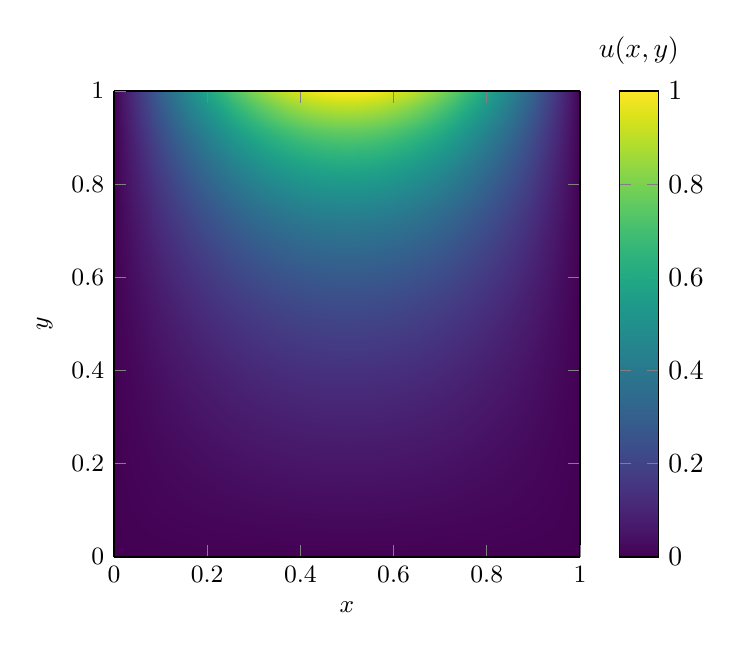
\begin{tikzpicture}
\begin{axis}[
  width=8.5cm, height=7.5cm,
  view={0}{90},
  xlabel={$x$},
  ylabel={$y$},
  xmin=0, xmax=1,
  ymin=0, ymax=1,
  axis equal image,
  colormap/viridis,
  colorbar,
  colorbar style={
    title={$u(x,y)$},
    ytick={0,0.2,0.4,0.6,0.8,1.0},
  },
  font=\small,
  point meta min=0, point meta max=1,
]
\addplot3[
  surf, shader=interp,
  samples=60, samples y=60,
  domain=0:1, y domain=0:1,
] { sin(deg(pi*x)) * sinh(pi*y) / sinh(pi) };
\end{axis}
\end{tikzpicture}
\caption[Laplace solution on a unit square]{Steady-state solution
of $\laplacian u = 0$ on the unit square with boundary data
$u(x,0) = u(0,y) = u(1,y) = 0$ and $u(x,1) = \sin(\pi x)$, obtained
by separation of variables as $u(x,y) = \sin(\pi x)\sinh(\pi
y)/\sinh(\pi)$. The colour map shows the field. The maximum
principle is satisfied: the field attains its maximum $u = 1$ on
the top boundary at $x = 1/2$, its minimum $u = 0$ on the other
three edges, and every interior value lies strictly between. The
exponential-style decay of the sinh ratio sets the penetration
depth of the boundary detail into the interior.}
\label{fig:vol02:ch12:laplace-square}
\end{figure}


\Cref{fig:vol02:ch12:laplace-square} gives the working picture.
The boundary detail (a half-sine on the top edge) penetrates into
the rectangle with decay length set by the wavelength of the
boundary mode. A boundary disturbance of higher spatial frequency
would decay faster into the interior; a slower disturbance would
penetrate further. The same low-pass character that the heat
equation exhibits in time, Laplace's equation exhibits in space.

\subsection{Worked example: the total heat rate through a plate edge}\pathtag{standard}

The square-plate solution gives the temperature field, but the number
an engineer usually needs is the heat rate, the total power crossing a
boundary, and computing it turns the harmonic field into a flux
integral. Take the same plate solution $u(x, y) = \sin(\pi x)
\sinh(\pi y)/\sinh(\pi)$ on the unit square, with conductivity $k$ and
unit thickness. The local heat flux leaving the hot top edge $y = 1$
is $q_{y} = -k\, u_{y}$ evaluated there,
\[
u_{y}(x, 1) = \pi\sin(\pi x)\,\frac{\cosh(\pi)}{\sinh(\pi)}
            = \pi\sin(\pi x)\coth(\pi),
\]
so the flux is largest at the centre of the edge, where the boundary
temperature peaks, and vanishes at the corners. The total heat rate
leaving the top edge is the integral of the flux along it,
\[
Q_{\text{top}} = -\int_{0}^{1} k\, u_{y}(x, 1)\,\dd x
        = -k\pi\coth(\pi)\int_{0}^{1}\sin(\pi x)\,\dd x
        = -k\pi\coth(\pi)\cdot\frac{2}{\pi}
        = -2k\coth(\pi).
\]
With $\coth(\pi) = 1.00374$ the top edge sheds $Q_{\text{top}} =
-2.0075\,k$ per unit temperature scale, the minus sign recording that
heat flows out of the domain across the heated edge (down the gradient
into the cooler interior). The same integral over the three cold edges
returns $+2.0075\,k$ in total, and the balance $Q_{\text{top}} +
Q_{\text{sides}} + Q_{\text{bottom}} = 0$ is not a coincidence: it is
the divergence theorem applied to a source-free harmonic field, whose
net boundary flux must vanish because $\int_{\Omega}\laplacian u\,\dd A
= 0$. The check is the working discipline. Any Laplace solve should be
audited by integrating the flux around the whole boundary and
confirming it sums to the enclosed source (zero for Laplace, the total
generation for Poisson); a non-zero residual on a source-free problem
signals a discretisation error or a boundary-condition mistake, and it
is the fastest sanity test on a numerical harmonic field.

\subsection{Worked example: the conduction shape factor for a buried pipe}\pathtag{standard}

The edge-integral of the previous example turned a harmonic field
into a total heat rate. When that heat rate is wanted for a fixed
geometry across many operating conditions, the field solve can be
done once and packed into a single geometric constant, the
\engterm{conduction shape factor}, which is the elliptic analogue of
the lumped conductance and the second appearance of the theme that a
distributed problem reduces to a lumped parameter once the field is
known. Consider a long isothermal pipe of radius $r$ at temperature
$T_{p}$ buried at depth $z$ (centre to surface) below flat ground held
at $T_{s}$. The steady temperature obeys Laplace's equation in the
soil, $\laplacian T = 0$, with $T = T_{p}$ on the pipe and $T = T_{s}$
on the surface. The domain is the half-plane with a circular hole, a
geometry that separation of variables in Cartesian or polar
coordinates does not fit, but that bipolar coordinates solve in closed
form. The result for the total heat rate per unit length is
\[
q' = S'\, k\,(T_{p} - T_{s}), \qquad
S' = \frac{2\pi}{\operatorname{arccosh}(z/r)},
\]
where $S'$ is the shape factor per unit length and $k$ the soil
conductivity. \Cref{fig:vol02:ch12:shape-factor} shows the isotherm
picture: eccentric circles crowding the warm pipe and spreading toward
the cool surface, the field that $S'$ summarises.

% Figure: the conduction shape factor for a cylinder of radius r
% buried at depth z below an isothermal ground surface. Isotherms of
% the harmonic potential are eccentric circles (bipolar coordinates);
% the surface is flat, the pipe is warm, and heat spreads outward.
% The shape factor S packs this whole field into a single conductance.
\begin{figure}[htbp]
\centering
\begin{tikzpicture}[>=Stealth, font=\small]
% Ground surface (isothermal, T_s), a horizontal line.
\draw[engblack, very thick] (-4.2,0) -- (4.2,0);
\node[anchor=south west, engblack] at (-4.2,0) {surface at $T_{s}$};
% Hatch above surface to mark the air / boundary side.
\foreach \x in {-4.0,-3.5,...,4.0}{
  \draw[engblack!45, thin] (\x,0) -- (\x+0.28,0.28);
}
% The buried pipe: a filled circle at depth z.
\fill[engred!22] (0,-2.4) circle (0.55);
\draw[engred, very thick] (0,-2.4) circle (0.55);
\node[engred] at (0,-2.4) {$T_{p}$};
% Depth annotation z from surface to pipe centre.
\draw[<->, engblack] (2.4,0) -- (2.4,-2.4);
\node[anchor=west, engblack] at (2.4,-1.2) {depth $z$};
% Radius annotation.
\draw[<->, engblue] (0,-2.4) -- (0.55,-2.4);
\node[anchor=north, engblue] at (0.30,-2.55) {$r$};
% Isotherms: eccentric circles crowding the pipe, widening toward the
% surface. Drawn as ellipse-like arcs at increasing radius and rising
% centre to suggest the bipolar family.
\draw[engblue!70, thick]   (0,-2.4) ellipse (0.95 and 0.85);
\draw[engblue!55, thick]   (0,-2.15) ellipse (1.55 and 1.30);
\draw[engblue!40, thick]   (0,-1.75) ellipse (2.35 and 1.70);
\draw[engblue!30, thick]   (0,-1.30) ellipse (3.30 and 1.10);
\node[anchor=west, engblue!60] at (1.7,-2.35) {isotherms};
\end{tikzpicture}
\caption[Conduction shape factor for a buried cylinder]{Steady heat
conduction from an isothermal cylinder of radius $r$ buried at depth
$z$ below an isothermal ground surface, a two-dimensional Laplace
problem on the semi-infinite domain. The isotherms (blue) are the
level sets of the harmonic potential; they crowd against the warm pipe
and spread as eccentric circles toward the cool surface, the picture
that the bipolar-coordinate solution makes exact. The entire field
collapses into a single number, the conduction shape factor
$S = 2\pi/\operatorname{arccosh}(z/r)$, so that the total heat rate is
$q = S k (T_{p} - T_{s})$: a distributed Laplace field reduced to one
lumped conductance $Sk$. The engineer sizing a buried steam line or a
ground-loop heat exchanger reads the loss from $S$ alone, with no
field solve per case.}
\label{fig:vol02:ch12:shape-factor}
\end{figure}


The number does the work. Take a steam line of radius $r =
0.15\,\si{\meter}$ buried at $z = 1.0\,\si{\meter}$ in soil of
conductivity $k = 1.2\,\si{\watt\per\meter\per\kelvin}$, carrying
steam at $T_{p} = 150\,{}^{\circ}\mathrm{C}$ under ground at $T_{s} =
10\,{}^{\circ}\mathrm{C}$. The ratio $z/r = 6.67$ gives
$\operatorname{arccosh}(6.67) = \ln(6.67 + \sqrt{6.67^{2} - 1}) =
\ln(13.26) = 2.585$, so $S' = 2\pi/2.585 = 2.43$ per metre of run. The
heat loss is $q' = 2.43 \times 1.2 \times (150 - 10) = 408\,\si{\watt}$
per metre. A one-kilometre run sheds $408\,\si{\kilo\watt}$ to the
ground, the number that sizes the insulation and prices the standing
loss. The shape factor also exposes the levers by inspection: because
$S'$ depends on depth and radius only through $\operatorname{arccosh}
(z/r)$, and $\operatorname{arccosh}$ grows logarithmically, doubling
the burial depth from $z/r = 6.67$ to $13.3$ changes
$\operatorname{arccosh}$ from $2.585$ to $3.28$ and cuts the loss only
to $302\,\si{\watt}$ per metre, a $26\,\%$ reduction for twice the
trenching. Insulation, which multiplies the resistance directly, buys
far more per unit cost than burial depth, and the shape factor shows
why before any money is spent. The catalogue of shape factors for
common geometries (a sphere near a surface, parallel buried pipes, an
eccentric annulus, a disc on a half-space) is a standard table in
\textcite{text:incropera2007}; each entry is one Laplace solve done
once and reused as a conductance.

\subsection{Poisson's equation and the role of sources}

Laplace's equation describes a region free of sources. Where a
source is present, the equation acquires a right-hand side and
becomes \engterm{Poisson's equation}
\[
\laplacian u = -f,
\]
with $f$ the source density. In steady-state heat conduction,
$f = S/k$ with $S$ a volumetric heat-generation rate (in $\si{\watt
\per\meter\cubed}$): resistive heating in a wire, exothermic
reaction in a catalyst pellet, nuclear heating in a fuel rod. In
electrostatics, $\laplacian \phi = -\rho/\varepsilon_{0}$ with
$\rho$ the charge density, the form the reader meets again in
Volume VII. In structural mechanics, the deflection of a uniformly
loaded membrane satisfies Poisson's equation with $f$ the pressure
over the tension.

The general solution of a Poisson problem splits into a particular
solution that carries the source and a harmonic solution that fits
the boundary. A worked instance: a slab $0 \leq x \leq L$ with
uniform internal generation $S$, both faces held at $0$, satisfies
$k\, u'' = -S$ in steady state, integrating to the parabolic profile
\[
u(x) = \frac{S}{2k}\, x\,(L - x),
\]
with peak $u_{\max} = S L^{2}/(8k)$ at the centre. The profile is a
downward parabola pinned to zero at both ends, the steady
temperature of a current-carrying busbar or a self-heating
battery cell cooled at its faces. The peak scales as $L^{2}$, so
halving the cooled spacing quarters the central temperature rise,
the working lever the thermal engineer pulls when a generation rate
is fixed and the centre is running too hot.

\subsection{Applied vignette: the thermal-runaway threshold of a battery cell}\pathtag{standard}

The Poisson slab of the previous subsection assumed the generation
rate $S$ was fixed. In a lithium-ion cell, a compost heap, or a
stored reactive solid the generation is not fixed: it rises with
temperature, because the exothermic reaction that produces the heat
speeds up as it warms. That feedback turns the benign Poisson problem
into a threshold problem with a sharp tipping point, and locating the
tipping point before the cell is built is the working payoff of the
elliptic prototype for the safety engineer.

\textbf{The self-heating balance.} Model a cell as a slab
$-L \leq x \leq L$ with faces held at ambient $T_{0}$ by the cooling
system, generating heat at an Arrhenius rate $S(T) = S_{0}\exp(-E_{a}
/RT)$ that climbs steeply with temperature. The steady heat equation
with this source is
\[
k\, u'' + S_{0}\, e^{-E_{a}/RT} = 0, \qquad u(\pm L) = T_{0}.
\]
The nonlinearity is the exponential, and the standard reduction,
after Frank-Kamenetskii, linearises the Arrhenius exponent about the
ambient temperature. Writing the dimensionless excess $\theta =
(E_{a}/RT_{0}^{2})(T - T_{0})$ and the \engterm{Frank-Kamenetskii
parameter}
\[
\delta = \frac{E_{a}}{RT_{0}^{2}}\,\frac{S_{0}\, e^{-E_{a}/RT_{0}}\, L^{2}}{k},
\]
which bundles the reaction rate, the cell size, the cooling
temperature, and the conductivity into one group, the balance becomes
the parameter-free Poisson-with-exponential-source equation $\theta''
+ \delta\, e^{\theta} = 0$ with $\theta(\pm 1) = 0$.

\textbf{The threshold.} The equation has a closed-form solution, and
its structure is the whole story. \Cref{fig:vol02:ch12:runaway} reads
the balance as heat generated (the exponential) against heat conducted
away (which, linearised, rises with the centre excess). Below a
critical $\delta$ the two curves cross twice: a stable low-temperature
steady state, where a small warming is out-conducted and the cell
settles, and an unstable high one. At the critical value the curves
become tangent, the two steady states merge, and for any larger
$\delta$ the generation exceeds the conduction at every temperature so
no steady state exists: the cell heats without bound. The critical
value for the slab is
\[
\delta_{c} = 0.878,
\]
(the plane-slab Frank-Kamenetskii number; a cylinder gives $2.00$ and
a sphere $3.32$, the geometry entering through the same Laplacian that
set the disk and sphere eigenvalues earlier). A cell operating at
$\delta < \delta_{c}$ is thermally stable; one pushed past
$\delta_{c}$ runs away.

\textbf{The design levers.} Every term in $\delta$ is a lever, and
the $L^{2}$ dependence is the sharpest. Because $\delta \propto L^{2}$,
a cell twice as thick sits at four times the parameter: scaling a
stable small cell up in size is the classic path into runaway, which
is why large-format cells and dense battery packs demand cooling that
a single small cell never needed. The ambient temperature enters
through both the explicit $T_{0}^{2}$ and the far stronger Arrhenius
$e^{-E_{a}/RT_{0}}$, so a modest rise in coolant temperature can
multiply $\delta$ severalfold and carry a cell that was safe at
$25\,\degC$ past threshold at $45\,\degC$, the mechanism behind
warm-ambient pack failures. The conductivity $k$ and the cell size
$L$ are the designer's controllable levers: raising $k$ (better
internal thermal paths) or lowering $L$ (thinner electrodes, more
cooling channels) drops $\delta$ below $\delta_{c}$ with margin. The
working discipline is to compute $\delta$ for the worst-case ambient
and confirm it sits safely below the geometry's critical value, with
a margin that covers the uncertainty in $S_{0}$ and $E_{a}$, which for
a real cell chemistry are measured by calorimetry and carry their own
error bands. The elliptic self-heating problem does not merely predict
a temperature; it predicts whether a steady temperature exists at all,
and that existence question is the safety margin.

% Figure: the Frank-Kamenetskii self-heating balance. The heat a
% slab loses by conduction (a line in the central-temperature excess)
% against the heat an Arrhenius reaction generates (an exponential),
% for three values of the generation parameter delta. Below the
% critical delta two steady states exist (a stable low one and an
% unstable high one); above it the generation curve clears the loss
% line everywhere and no steady state exists: thermal runaway.
\begin{figure}[htbp]
\centering
\begin{tikzpicture}
\begin{axis}[
  width=12cm, height=6.5cm,
  xlabel={dimensionless centre excess $\theta$},
  ylabel={dimensionless heat rate},
  xmin=0, xmax=6, ymin=0, ymax=6,
  grid=both,
  major grid style={engblack!20}, minor grid style={engblack!10},
  legend pos=north west, legend cell align=left,
  font=\small, samples=160, domain=0:6,
]
% Conductive loss: proportional to theta (linearised), slope 1.
\addplot[engblack, thick] { x };
\addlegendentry{conductive loss $\propto \theta$}
% Generation: delta * exp(theta) (Frank-Kamenetskii exponential).
% Sub-critical delta = 0.2: two crossings.
\addplot[engblue, very thick] { 0.2*exp(x) };
\addlegendentry{generation, $\delta = 0.2$ (sub-critical)}
% Critical delta_c = 1/e = 0.368: tangent to the loss line.
\addplot[engorange, very thick, dashed] { 0.3679*exp(x) };
\addlegendentry{generation, $\delta_c = 1/e$ (tangent)}
% Super-critical delta = 0.6: no crossing, runaway.
\addplot[engred, very thick, dotted] { 0.6*exp(x) };
\addlegendentry{generation, $\delta = 0.6$ (runaway)}
\end{axis}
\end{tikzpicture}
\caption[Thermal-runaway balance]{Self-heating balance for a
reacting slab (the Frank-Kamenetskii model). The straight line is
the heat conduction carries away, rising with the dimensionless
centre excess $\theta$; the curves are the heat an Arrhenius reaction
generates, $\delta\, e^{\theta}$, for three values of the generation
parameter $\delta$. At the sub-critical $\delta = 0.2$ the curve
crosses the loss line twice: the lower crossing is a stable steady
state, the upper an unstable one. At the critical $\delta_c = 1/e$
the curve is tangent to the line, the two steady states merge, and
any further increase leaves the generation above the loss for every
$\theta$, so no steady state exists and the temperature climbs
without bound. Crossing $\delta_c$ is the tipping point of thermal
runaway in a battery cell, a compost pile, or a stored reactive
solid, and the Poisson self-heating problem locates it before the
cell is built.}
\label{fig:vol02:ch12:runaway}
\end{figure}


\subsection{Worked example: the discrete mean-value property}

The mean-value property has a discrete shadow that is the
foundation of every relaxation solver for Laplace's equation. On a
uniform grid with spacing $h$, the five-point Laplacian is
\[
\laplacian u(x_{i}, y_{j}) \approx \frac{U_{i+1,j} + U_{i-1,j} + U_{i,j+1} + U_{i,j-1} - 4 U_{i,j}}{h^{2}}.
\]
Setting this to zero (the discrete Laplace equation) and solving for
the centre value gives
\[
U_{i,j} = \frac{1}{4}\bigl(U_{i+1,j} + U_{i-1,j} + U_{i,j+1} + U_{i,j-1}\bigr).
\]
The discrete harmonic value at any node is the average of its four
neighbours, the exact discrete analogue of the continuous
mean-value property. The discrete maximum principle follows by the
same argument as the continuous one: a discrete harmonic function
cannot have an interior node strictly larger than all its
neighbours, so its extrema sit on the boundary. The Jacobi
iteration of \S12.7 simply applies the averaging rule repeatedly
until the field stops changing, which is the numerical statement
that the field has become discretely harmonic. The reader who has
seen a relaxation solver "settle" a temperature field into a smooth
equilibrium has watched the discrete mean-value property converge.

A quick application: a square plate with three edges at $0$ and one
edge at $100$, discretised on the coarsest non-trivial grid (a
single interior node by symmetry on a $3 \times 3$ mesh), gives that
node the value $\tfrac{1}{4}(100 + 0 + 0 + 0) = 25\,\degC$, the same
quarter-of-the-boundary answer the exact symmetry argument produces
for the plate centre. The coarsest discretisation already carries
the right answer at the centre because the symmetry that fixes it is
preserved by the five-point stencil.

\subsection{Case study: seepage under a dam, a Laplace problem on a real domain}\pathtag{standard}

Laplace's equation governs more than temperature and potential; in
soil it governs the flow of water under a structure, and the
seepage-under-a-dam problem is the classical civil-engineering
application that turns the abstract harmonic field into a foundation
that does or does not wash out. The case earns a full pass because
it shows the maximum principle, the flux integral, and the numerical
relaxation working together on a domain an engineer actually pours
concrete on.

\textbf{The physics and the governing equation.} Water seeping
through saturated soil obeys \engterm{Darcy's law}, the
constitutive relation that the volumetric flux (the Darcy velocity)
is proportional to the gradient of the \engterm{hydraulic head} $h$,
\[
\mathbf{q} = -K\,\grad h,
\]
with $K$ the hydraulic conductivity, in $\si{\meter\per\second}$,
the same form as Fourier's law with head in place of temperature
and conductivity in place of thermal conductivity. Conservation of
incompressible water, $\divg\mathbf{q} = 0$, then gives Laplace's
equation for the head,
\[
\laplacian h = 0,
\]
on the soil region beneath and beside the dam. The analogy is exact:
head plays temperature, Darcy conductivity plays thermal
conductivity, and the flux integral plays the heat rate. Everything
the chapter proved about harmonic functions transfers.

\textbf{The domain and boundary conditions.} Consider a concrete
gravity dam founded on a permeable soil layer of depth $D$ over an
impermeable bedrock. Upstream the reservoir stands at head $h =
H_{1}$; downstream the tailwater stands at $h = H_{2} < H_{1}$. The
soil region is the rectangle below the ground surface, bounded above
by the soil-structure interface and the two channel bottoms, and
below by bedrock. The boundary conditions read straight off the
physics. The upstream soil surface, in contact with the reservoir,
is Dirichlet at $h = H_{1}$; the downstream soil surface is Dirichlet
at $h = H_{2}$; the impermeable bedrock and the base of the dam
itself are Neumann with zero normal flux, $\partial h/\partial n =
0$, because no water crosses an impermeable face. The seepage problem
is thus a mixed Dirichlet-Neumann Laplace problem on a rectangular
soil block with the dam base as an internal no-flow segment along
the top.

\textbf{What the maximum principle gives for free.} Before any
computation, the maximum principle bounds the head everywhere in the
soil between $H_{2}$ and $H_{1}$: no interior point can carry a head
above the reservoir or below the tailwater. The working consequence
is the \engterm{uplift pressure} on the dam base. The head along the
base, interpolating from $H_{1}$ at the upstream heel to $H_{2}$ at
the downstream toe, sets the pore-water pressure pushing up on the
foundation, and the integral of that pressure is the uplift force
that a gravity dam must out-weigh. A dam designed without accounting
for uplift, computed from exactly this harmonic head field, is a dam
that floats; the failure mode is real and historical, and the
head-field integral is the load the structural check consumes.

\textbf{Solving by relaxation and reading the flow net.} On a
rectangular soil block the head field is found by the same Jacobi or
Gauss-Seidel relaxation that solved the steady-temperature plate, now
with the no-flow Neumann condition implemented as a reflected ghost
node ($h_{\text{ghost}} = h_{\text{interior}}$) along the bedrock and
the dam base. The converged field is read as a \engterm{flow net},
the orthogonal grid of equipotential lines (curves of constant head,
the isotherms of the analogy) and streamlines (paths the water
follows, perpendicular to the equipotentials). The total seepage
discharge is the flux integral across any equipotential,
\[
Q = \oint_{\text{cut}} \mathbf{q}\cdot\unitvec{n}\,\dd s
  = K\,(H_{1} - H_{2})\,\frac{N_{f}}{N_{d}},
\]
where $N_{f}$ is the number of flow channels and $N_{d}$ the number
of head drops in the net, the working flow-net formula. A concrete
number: a dam with head difference $H_{1} - H_{2} = 8\,\si{\meter}$
on a soil of conductivity $K = 10^{-5}\,\si{\meter\per\second}$, with
a flow net showing $N_{f} = 4$ channels and $N_{d} = 12$ drops, leaks
$Q = 10^{-5}\cdot 8\cdot (4/12) \approx 2.7\times 10^{-5}\,\si{\meter
\cubed\per\second}$ per metre of dam width, about $2.3\,\si{\meter
\cubed}$ per metre per day. The same field gives the exit gradient at
the downstream toe, the steepest head gradient in the net, which must
stay below the critical gradient at which the soil grains lift and
\engterm{piping} begins, the erosion channel that has failed earthen
dams. The harmonic head field, the maximum-principle uplift bound,
the flux-integral discharge, and the exit-gradient piping check are
four engineering deliverables read off one Laplace solve, and they
are why the seepage problem is the canonical civil application of the
elliptic prototype.

\section{Separation of variables, Fourier series introduction}\pathtag{core}

Separation of variables is the workhorse method for solving the
canonical boundary-value problems for the heat, wave, and Laplace
equations on rectangular domains. The method assumes the solution
factors as a product of single-variable functions, derives an
ordinary differential equation for each factor, and assembles the
general solution as an infinite series of separable building
blocks. The series-summation step uses Fourier series, the working
expansion of a periodic or boundary-fitted function in
trigonometric harmonics.

\subsection{Heat equation on a finite rod: the canonical example}

Consider $u_{t} = \alpha u_{xx}$ on $0 \leq x \leq L$, $t \geq 0$,
with boundary conditions $u(0, t) = u(L, t) = 0$ and initial
condition $u(x, 0) = f(x)$. Try the separated form $u(x, t) =
X(x) T(t)$. Substituting:
\[
X(x) T'(t) = \alpha\, X''(x)\, T(t),
\]
and rearranging,
\[
\frac{T'(t)}{\alpha\, T(t)} = \frac{X''(x)}{X(x)}.
\]
The left-hand side depends only on $t$, the right-hand side only
on $x$. The equation can hold for all $t$ and $x$ only if both
sides equal a common constant; call it $-\lambda$ (the minus sign
chosen with foresight; $\lambda > 0$ will give decaying solutions).
We get two ordinary differential equations:
\[
T'(t) = -\alpha \lambda\, T(t), \qquad X''(x) = -\lambda\, X(x).
\]
The first integrates immediately to $T(t) = T(0) e^{-\alpha \lambda
t}$. The second is the eigenvalue problem
\[
X''(x) + \lambda X(x) = 0, \qquad X(0) = X(L) = 0,
\]
where the boundary conditions on $X$ come from $u(0, t) = u(L, t)
= 0$ (which must hold for all $t$, hence for $X$ alone). The
nontrivial solutions are
\[
X_{n}(x) = \sin\!\left(\frac{n \pi x}{L}\right), \qquad \lambda_{n} = \left(\frac{n \pi}{L}\right)^{2}, \qquad n = 1, 2, 3, \ldots.
\]
Each pair $(X_{n}, \lambda_{n})$ gives a separable solution
\[
u_{n}(x, t) = \sin\!\left(\frac{n \pi x}{L}\right) \exp\!\left(-\alpha \left(\frac{n \pi}{L}\right)^{2} t\right).
\]
The general solution is a superposition:
\[
u(x, t) = \sum_{n = 1}^{\infty} b_{n}\, \sin\!\left(\frac{n \pi x}{L}\right) \exp\!\left(-\alpha \left(\frac{n \pi}{L}\right)^{2} t\right),
\]
with the coefficients $b_{n}$ determined by matching the initial
condition $u(x, 0) = f(x)$:
\[
f(x) = \sum_{n = 1}^{\infty} b_{n} \sin\!\left(\frac{n \pi x}{L}\right).
\]
This is the Fourier sine series of $f$ on $[0, L]$. The
coefficients are
\[
b_{n} = \frac{2}{L} \int_{0}^{L} f(x) \sin\!\left(\frac{n \pi x}{L}\right) \dd x.
\]
The factor $2/L$ comes from the orthogonality relation
$\int_{0}^{L} \sin(n\pi x/L) \sin(m\pi x/L)\, \dd x = (L/2)
\delta_{nm}$, derived in standard texts \cite{text:strang2016}.

The construction is general: every boundary condition admits a
family of eigenfunctions $X_{n}$, and the coefficients are the
inner products of the data against the eigenfunctions.

% Figure: the first four eigenfunctions sin(n pi x/L) of the
% separation-of-variables problem with Dirichlet boundary
% conditions on [0,L]. Drawn together with their relative time
% constants tau_n / tau_1 = 1/n^2.
\begin{figure}[htbp]
\centering
\begin{tikzpicture}
\begin{axis}[
  width=11cm, height=6cm,
  xlabel={position $x/L$},
  ylabel={mode $X_n(x) = \sin(n \pi x/L)$},
  xmin=0, xmax=1,
  ymin=-1.1, ymax=1.4,
  grid=both,
  major grid style={engblack!20},
  minor grid style={engblack!10},
  legend pos=north east,
  legend cell align=left,
  font=\small,
  samples=200,
  domain=0:1,
]
\addplot[engblue, very thick]               {sin(deg(pi*x))};
\addlegendentry{$n=1$,\ $\tau_1/\tau_1 = 1$}
\addplot[engred, very thick]                {sin(deg(2*pi*x))};
\addlegendentry{$n=2$,\ $\tau_2/\tau_1 = 1/4$}
\addplot[engblue!60!engblack, thick, dashed]{sin(deg(3*pi*x))};
\addlegendentry{$n=3$,\ $\tau_3/\tau_1 = 1/9$}
\addplot[engred!60!engblack, thick, dashed] {sin(deg(4*pi*x))};
\addlegendentry{$n=4$,\ $\tau_4/\tau_1 = 1/16$}

% Annotation indicating low-pass character.
\node[engblack, font=\scriptsize, align=left, anchor=west]
  at (axis cs:0.02, 1.25)
  {high modes decay faster:\ heat equation is low-pass};
\end{axis}
\end{tikzpicture}
\caption[Separation-of-variables eigenmodes]{The first four
eigenfunctions of $X'' + \lambda X = 0$ on $[0, L]$ with $X(0) =
X(L) = 0$. Each mode $X_n(x) = \sin(n\pi x/L)$ is a standing wave
with $n$ half-wavelengths fitting between the boundaries. Under
the heat equation, mode $n$ decays exponentially with time
constant $\tau_n = L^{2}/(\pi^{2} n^{2} \alpha) = \tau_1/n^{2}$;
under the wave equation, mode $n$ oscillates at frequency
$\omega_n = c n \pi/L = n \omega_1$. The same eigenbasis carries
both the parabolic decay structure (heat) and the hyperbolic
harmonic structure (vibrating string).}
\label{fig:vol02:ch12:separation-modes}
\end{figure}


\subsection{Why the time constants stack as $1/n^{2}$}

The mode $u_{n}$ decays with time constant $\tau_{n} = 1/(\alpha
\lambda_{n}) = L^{2}/(\alpha (n \pi)^{2})$. The fundamental mode
($n = 1$) has the longest time constant, $\tau_{1} = L^{2}/(\pi^{2}
\alpha)$. The next mode decays $4\times$ faster, the next $9\times$,
and so on. After one $\tau_{1}$, the fundamental has dropped to
$1/e$ of its initial amplitude; the higher modes are vanishingly
small. The heat equation is, in a working sense, low-pass: high
spatial frequencies decay much faster than low ones, and the
late-time profile is dominated by the slowest mode. This
$1/n^{2}$ stacking is why the simple-engineer estimate "one time
constant" is reliable for the late-time behaviour of a parabolic
system, and why a rough Fourier series truncated to a few modes
is adequate at intermediate times.

\subsection{Wave equation on a finite string}

The wave equation $u_{tt} = c^{2} u_{xx}$ on $0 \leq x \leq L$
with $u(0, t) = u(L, t) = 0$, $u(x, 0) = \phi(x)$, $u_{t}(x, 0) =
\psi(x)$ separates the same way. The eigenvalue problem for $X$
is identical, giving $X_{n} = \sin(n \pi x/L)$ and $\lambda_{n} =
(n \pi/L)^{2}$. The time-equation $T''(t) = -c^{2} \lambda_{n}\,
T(t)$ has solutions $T_{n}(t) = a_{n} \cos(\omega_{n} t) + b_{n}
\sin(\omega_{n} t)$ with $\omega_{n} = c\, n \pi/L = c \sqrt
{\lambda_{n}}$. The general solution:
\[
u(x, t) = \sum_{n = 1}^{\infty} \sin\!\left(\frac{n \pi x}{L}\right) \bigl(a_{n} \cos(\omega_{n} t) + b_{n} \sin(\omega_{n} t)\bigr),
\]
with $a_{n}$ from the Fourier sine series of $\phi$ and
$\omega_{n} b_{n}$ from the Fourier sine series of $\psi$. The
modes are sinusoidal in time at frequencies $\omega_{n}$ that are
integer multiples of the fundamental $\omega_{1}$. The string
sustains a harmonic series; that is what makes it musical. The
$1/n^{2}$ amplitude pattern of the midpoint-plucked triangle, with
no even modes, is the signature audible in plucked-string acoustics.

\subsection{Laplace's equation in a rectangle}

Laplace's equation $u_{xx} + u_{yy} = 0$ on the rectangle $[0, L]
\times [0, M]$ separates as $u(x, y) = X(x) Y(y)$. Substituting:
\[
\frac{X''(x)}{X(x)} = -\frac{Y''(y)}{Y(y)} = -\lambda.
\]
The choice of sign on $\lambda$ depends on which pair of edges
carries the inhomogeneous data. With $u = 0$ on the left, right,
and bottom edges and $u(x, M) = g(x)$ on the top edge, the
$X$-eigenvalue problem inherits the boundary conditions $X(0) =
X(L) = 0$, giving $X_{n} = \sin(n\pi x/L)$ and $\lambda_{n} =
(n\pi/L)^{2}$. The $Y$-equation is then $Y_{n}'' = \lambda_{n}
Y_{n}$, with solutions $\sinh(n\pi y/L)$ and $\cosh(n\pi y/L)$.
The boundary $Y(0) = 0$ pins to $\sinh(n\pi y/L)$. The general
solution is
\[
u(x, y) = \sum_{n = 1}^{\infty} c_{n} \sin\!\left(\frac{n \pi x}{L}\right) \frac{\sinh(n \pi y/L)}{\sinh(n \pi M/L)},
\]
with $c_{n}$ the Fourier sine coefficients of $g(x)$. The sinh
ratio is the working analogue of the exponential decay in the
heat case: in the Laplace case the field "decays" away from the
inhomogeneous boundary into the rectangle, with the decay length
set by the wavelength of the boundary mode. High-frequency
boundary detail decays into the rectangle faster than low-frequency
detail, the same low-pass character that the heat equation
exhibits in time.

\subsection{Worked example: a two-mode boundary on the square, end to end}

The single-mode plate of §12.4 hides the most useful working fact
about Laplace's equation, that the interior is a low-pass filter of
the boundary data. A two-mode boundary makes it visible. Take the
unit square $[0,1]\times[0,1]$ with $u = 0$ on the left, right, and
bottom edges and the top edge carrying
\[
g(x) = \sin(\pi x) - \tfrac{1}{2}\sin(3\pi x).
\]
The data are already a finite Fourier sine series, so no integral
is needed: $c_{1} = 1$ on the $n = 1$ mode and $c_{3} = -\tfrac{1}{2}$
on the $n = 3$ mode, all others zero. The rectangle solution from
the separation formula, with $M = 1$, is
\[
u(x, y) = \sin(\pi x)\, \frac{\sinh(\pi y)}{\sinh(\pi)}
        - \tfrac{1}{2}\sin(3\pi x)\, \frac{\sinh(3\pi y)}{\sinh(3\pi)}.
\]
Each mode carries its own $\sinh$ envelope, and the envelopes decay
into the interior at rates set by the mode number. At the boundary
$y = 1$ both $\sinh$ ratios are one and the field reproduces $g$. At
the mid-height $y = \tfrac{1}{2}$ the fundamental envelope is
$\sinh(\pi/2)/\sinh(\pi) = 2.301/11.549 \approx 0.199$, while the
third-mode envelope is $\sinh(3\pi/2)/\sinh(3\pi) = 55.65/6195.8
\approx 8.98 \times 10^{-3}$, a factor of twenty-two smaller
relative to its boundary amplitude. The third harmonic has been
filtered out: at mid-height the field is, to better than one
percent, a clean half-sine. \Cref{fig:vol02:ch12:laplace-twomode}
traces the field along four horizontal cuts and shows the dip from
the third harmonic vanishing within a quarter of the way down.

The general statement: mode $n$ decays into the rectangle with
characteristic length $L/(n\pi)$, so a boundary feature of spatial
wavelength $\ell$ penetrates a depth of order $\ell/(2\pi)$ before
it is attenuated. An engineer reading a measured surface
temperature field to infer conditions a few centimetres inside a
wall recovers only the long-wavelength part of the surface data;
the short-wavelength detail has been erased by the same elliptic
smoothing, and any attempt to recover it from interior measurements
is the spatial analogue of the ill-posed backward heat problem of
§12.8.

% Figure: 2-D Laplace solution on a rectangle with a two-mode top
% boundary. Plots the interior field along three horizontal cuts and
% shows how the higher boundary mode decays faster into the interior.
\begin{figure}[htbp]
\centering
\begin{tikzpicture}
\begin{axis}[
  width=12cm, height=6.5cm,
  xlabel={position $x/L$},
  ylabel={temperature $u(x,y)$},
  xmin=0, xmax=1,
  ymin=-0.45, ymax=1.05,
  grid=both,
  major grid style={engblack!20},
  minor grid style={engblack!10},
  legend pos=south east,
  legend cell align=left,
  font=\small,
  samples=160,
  domain=0:1,
]
% Boundary data on top edge: g(x) = sin(pi x) - 0.5 sin(3 pi x).
% Solution u(x,y) = sin(pi x) sinh(pi y)/sinh(pi)
%                 - 0.5 sin(3 pi x) sinh(3 pi y)/sinh(3 pi).
% sinh(pi)=11.5487, sinh(3pi)=6195.82.
\addplot[engblack, very thick, dashed] {
  sin(deg(pi*x)) - 0.5*sin(deg(3*pi*x))
};
\addlegendentry{$y/M = 1$ (boundary data $g$)}

\addplot[engred, very thick] {
    sin(deg(pi*x))   * (sinh(pi*0.75)/11.5487)
  - 0.5*sin(deg(3*pi*x)) * (sinh(3*pi*0.75)/6195.82)
};
\addlegendentry{$y/M = 0.75$}

\addplot[engblue, very thick] {
    sin(deg(pi*x))   * (sinh(pi*0.5)/11.5487)
  - 0.5*sin(deg(3*pi*x)) * (sinh(3*pi*0.5)/6195.82)
};
\addlegendentry{$y/M = 0.5$}

\addplot[engblue!55!engblack, very thick, dotted] {
    sin(deg(pi*x))   * (sinh(pi*0.25)/11.5487)
  - 0.5*sin(deg(3*pi*x)) * (sinh(3*pi*0.25)/6195.82)
};
\addlegendentry{$y/M = 0.25$}

\end{axis}
\end{tikzpicture}
\caption[Two-mode Laplace boundary penetration]{Steady Laplace field
on the unit square with the two-mode top-edge data $g(x) = \sin(\pi
x) - \tfrac{1}{2}\sin(3\pi x)$ and zero on the other three edges.
Each curve is a horizontal cut at a fixed height $y/M$. At the
boundary ($y/M = 1$, dashed) both modes are present and the dip from
the third harmonic is visible. One quarter of the way down ($y/M =
0.75$) the third mode has already shrunk by $\sinh(3\pi\cdot
0.75)/\sinh(3\pi) \approx 0.10$ against the fundamental's
$\sinh(\pi\cdot 0.75)/\sinh(\pi) \approx 0.62$, so the cut is nearly
a clean half-sine. By mid-height the third mode is below one part in
a hundred. High-spatial-frequency boundary detail decays into the
interior faster than low-frequency detail; the decay length of mode
$n$ is $L/(n\pi)$, the same low-pass behaviour the heat equation
shows in time.}
\label{fig:vol02:ch12:laplace-twomode}
\end{figure}


\subsection{Worked example: separation of variables in polar coordinates}\pathtag{standard}

Separation of variables adapts to curved boundaries: a wedge or a
disk separates in polar coordinates, and the eigenfunctions follow
the boundary shape.
Laplace's equation in the plane, written in polar coordinates
$(r, \phi)$, is
\[
\laplacian u = u_{rr} + \frac{1}{r}\, u_{r} + \frac{1}{r^{2}}\, u_{\phi\phi} = 0.
\]
Try $u(r, \phi) = R(r)\, \Phi(\phi)$. Substituting and multiplying
by $r^{2}/(R\Phi)$,
\[
\frac{r^{2} R'' + r R'}{R} = -\frac{\Phi''}{\Phi} = \lambda,
\]
a separation constant $\lambda$. The angular equation $\Phi'' +
\lambda\Phi = 0$ with the periodicity condition $\Phi(\phi + 2\pi)
= \Phi(\phi)$ forces $\lambda = n^{2}$ for integer $n$, giving
$\Phi_{n} = \cos(n\phi)$ and $\sin(n\phi)$. The radial equation
$r^{2} R'' + r R' - n^{2} R = 0$ is an Euler equation with power-law
solutions $R = r^{n}$ and $r^{-n}$ (and $R = 1, \ln r$ for $n = 0$).
Boundedness at the centre of a disk discards the $r^{-n}$ branch,
leaving the interior solution
\[
u(r, \phi) = \frac{a_{0}}{2} + \sum_{n = 1}^{\infty} r^{n}\bigl(a_{n}\cos(n\phi) + b_{n}\sin(n\phi)\bigr),
\]
with the coefficients fixed by the boundary data on the rim $r = a$
through the ordinary Fourier series of $u(a, \phi)$, divided by the
geometric factor $a^{n}$. A concrete case: a unit disk with rim
temperature $u(1, \phi) = \cos\phi$ has the single-term solution
$u(r, \phi) = r\cos\phi = x$, harmonic and linear, the interior
field of a disk whose boundary is heated on one side and cooled on
the other. The mean-value property is visible: $u(0) = a_{0}/2 =
\tfrac{1}{2\pi}\int_{0}^{2\pi} u(a, \phi)\,\dd\phi$, the centre
value equals the rim average, here zero. The same separation, run on
a wedge of opening angle $\beta$ with zero data on the two straight
edges, produces eigenfunctions $\sin(m\pi\phi/\beta)$ and radial
powers $r^{m\pi/\beta}$; a re-entrant corner with $\beta > \pi$
gives a fractional power below one, the gradient singularity that
the L-shaped-domain design exercise of §12.9 must refine against.
The geometry chooses the eigenfunctions; the Sturm-Liouville
structure guarantees they still form an orthogonal basis.

\subsection{Worked example: the pipe wall as a Laplace problem on an annulus}\pathtag{standard}

The disk kept only the axis-regular radial branch; the annulus, the
region between two concentric circles, keeps both, and the mismatch
between the two branches is the working reason a curved wall behaves
differently from a flat one. Take steady conduction across a pipe
wall, inner radius $a$ at temperature $T_{a}$, outer radius $b$ at
$T_{b}$, with no angular variation. The axisymmetric Laplace equation
drops the $u_{\phi\phi}$ term and reads
\[
u_{rr} + \frac{1}{r}\, u_{r} = \frac{1}{r}\,\dv{}{r}\!\left(r\,\dv{u}{r}\right) = 0.
\]
The bracket is constant, so $r\, u_{r} = C_{1}$ and
$u(r) = C_{1}\ln r + C_{2}$: the harmonic radial profile is a
logarithm, the $n = 0$ radial solution of the polar development. The
boundary values $u(a) = T_{a}$, $u(b) = T_{b}$ fix the constants,
\[
u(r) = T_{b} + (T_{a} - T_{b})\,\frac{\ln(b/r)}{\ln(b/a)},
\]
plotted against fractional wall position in
\cref{fig:vol02:ch12:annulus}. The profile is not the straight line
of a flat slab; the logarithm bows it so the gradient is steepest at
the inner surface.

The gradient carries the engineering content. The heat flux is
$q(r) = -k\, u_{r} = k(T_{a} - T_{b})/[r\ln(b/a)]$, which falls as
$1/r$ across the wall, so the flux \emph{density} is largest at the
bore and smallest at the outer skin, while the total heat rate per
unit length, $Q' = 2\pi r q = 2\pi k(T_{a} - T_{b})/\ln(b/a)$, is
constant across the wall as conservation demands. The conductive
resistance per unit length is therefore $\ln(b/a)/(2\pi k)$, a
logarithm of the radius ratio rather than a wall thickness: doubling
the wall thickness of a thin large-bore pipe barely raises the
resistance, while the same doubling on a small-bore capillary changes
it substantially, because resistance tracks $\ln(b/a)$, not $b - a$.
A worked number: a steel pipe ($k = 45\,\si{\watt\per\meter\per
\kelvin}$) with $a = 10\,\si{\milli\meter}$, $b = 12\,\si{\milli
\meter}$ carrying $T_{a} - T_{b} = 60\,\si{\kelvin}$ rejects
$Q' = 2\pi\cdot 45\cdot 60/\ln(1.2) \approx 9.3\times
10^{4}\,\si{\watt\per\meter}$, and the inner-surface flux density is
$Q'/(2\pi a) \approx 1.5\times 10^{6}\,\si{\watt\per\meter\squared}$
against an outer-surface $1.2\times 10^{6}$, the twenty-percent bore
crowding that \cref{fig:vol02:ch12:annulus} shows for the thin-wall
curve. The same logarithmic harmonic solves the coaxial capacitor and
the radial groundwater flow to a well; the annulus is the elliptic
prototype in its second-simplest geometry, and its logarithm is the
signature of two-dimensional radial symmetry.

% Figure: steady radial temperature between two concentric cylinders
% (an annulus / pipe wall), the logarithmic harmonic profile, for
% three radius ratios. Contrasts with the linear profile of a slab:
% the curvature crowds the gradient onto the inner surface, which is
% why a thin pipe wall runs hotter on the bore side than a flat plate
% of the same thickness would.
\begin{figure}[htbp]
\centering
\begin{tikzpicture}
\begin{axis}[
  width=12cm, height=6.5cm,
  xlabel={fractional position across wall $(r-a)/(b-a)$},
  ylabel={dimensionless temperature $(T-T_b)/(T_a-T_b)$},
  xmin=0, xmax=1, ymin=0, ymax=1.05,
  grid=both,
  major grid style={engblack!20}, minor grid style={engblack!10},
  legend pos=north east, legend cell align=left,
  font=\small, samples=120, domain=0:1,
]
% Radial profile T = ln(b/r)/ln(b/a); parametrise r = a + s(b-a).
% Ratio b/a = 1.2 (thin wall). r(s) = 1 + 0.2 s, b = 1.2.
\addplot[engblue, very thick] { ln(1.2/(1+0.2*x)) / ln(1.2) };
\addlegendentry{$b/a = 1.2$ (thin wall)}
% b/a = 2. r(s) = 1 + s, b = 2.
\addplot[engorange, very thick, dashed] { ln(2/(1+x)) / ln(2) };
\addlegendentry{$b/a = 2$}
% b/a = 5. r(s) = 1 + 4s, b = 5.
\addplot[engred, very thick, dotted] { ln(5/(1+4*x)) / ln(5) };
\addlegendentry{$b/a = 5$ (thick wall)}
% Reference: the slab straight line.
\addplot[engblack, thin] { 1 - x };
\addlegendentry{flat slab (reference)}
\end{axis}
\end{tikzpicture}
\caption[Radial temperature in an annulus]{Steady radial temperature
across a cylindrical wall (annulus), the logarithmic harmonic profile
$T(r) = T_b + (T_a - T_b)\ln(b/r)/\ln(b/a)$, plotted against fractional
position for three radius ratios, with the flat-slab straight line
for reference. The curvature bows the profile below the slab line,
crowding the temperature gradient toward the inner (bore) surface: the
inner wall carries a steeper gradient and therefore a higher heat
flux per unit area than a flat wall of the same thickness would. The
effect grows with the radius ratio, which is why a small-bore
thick-walled pipe concentrates its thermal load on the bore and why
the conductive resistance of a pipe wall goes as $\ln(b/a)$ rather
than as the wall thickness.}
\label{fig:vol02:ch12:annulus}
\end{figure}


\begin{mastery}
The bowed annulus profile hides a subtlety about the second radial
branch. The interior disk problem discarded $\ln r$ because it
diverges at the centre, keeping the geometry regular; the exterior
problem (the field outside a cylinder, $r > a$, decaying at infinity)
discards the growing $r^{n}$ powers instead and keeps $r^{-n}$. The
annulus, having no centre and no infinity inside its domain, keeps
both branches for every angular mode, so its general axisymmetric
harmonic field is $u = C_{1}\ln r + C_{2} + \sum_{n\geq 1}
(A_{n}r^{n} + B_{n}r^{-n})(a_{n}\cos n\phi + b_{n}\sin n\phi)$, and
matching data on both circles determines all four constants per mode.
The working consequence appears when the two circles carry different
angular data: a uniform-field boundary condition on the outer circle
and a constant on the inner produces an $n = 1$ response with both an
$r$ and an $r^{-1}$ term, the superposition that models a conducting
or insulating cylindrical shell perturbing an applied field, the
two-dimensional cousin of the Legendre dielectric-sphere result. The
lesson the annulus teaches, that which radial branches survive is a
statement about the domain's topology (does it contain the origin, the
point at infinity, both, or neither), carries directly into the
method-of-images constructions and the multiply-connected potential
problems of the later field-theory volumes.
\end{mastery}

\subsection{Worked example: convergence rate set by data smoothness}\pathtag{standard}

How many Fourier terms a problem needs is read off the smoothness
of the data before any sum is taken. The coefficient decay rate and
the smoothness are tied by repeated integration by parts. For the
sine coefficients $b_{n} = (2/L)\int_{0}^{L} f \sin(n\pi x/L)\,\dd
x$, each integration by parts pulls out a factor $1/n$ and either a
boundary term or an integral of a derivative of $f$. A function
with a jump discontinuity loses at the first step: $b_{n} \sim 1/n$.
A continuous function with a kinked (discontinuous) first
derivative, the triangle, loses at the second step: $b_{n} \sim
1/n^{2}$. A function with $p$ continuous derivatives and a jump in
the $(p{+}1)$-th has $b_{n} \sim 1/n^{p+2}$.

The $L^{2}$ truncation error inherits the rate. By Parseval's
identity the squared error of the $N$-term partial sum is the tail
energy $\sum_{n > N} b_{n}^{2}$. For the jump datum, $\sum_{n > N}
n^{-2} \sim 1/N$, so $\|f - S_{N}\|_{2} \sim N^{-1/2}$. For the
triangle, $\sum_{n > N} n^{-4} \sim 1/N^{3}$, so $\|f - S_{N}\|_{2}
\sim N^{-3/2}$. \Cref{fig:vol02:ch12:fourier-convergence} plots both
on log-log axes; the slopes are $-1/2$ and $-3/2$, exactly the
integration-by-parts count. The working consequence: a square-wave
boundary needs roughly a hundred-fold more terms than a triangular
one to reach the same $L^{2}$ accuracy, and the only way to break
the slow rate is to change the data (smooth it) or change the basis
(a localised basis follows a jump without the global ringing). The
engineer who must resolve a sharp feature in a Fourier solution
counts the terms from this rate and budgets the work, or abandons
the global basis for a finite-element one.

% Figure: convergence of the Fourier sine series for a smooth (sine)
% datum versus a discontinuous (square) datum. Plots the L2 partial-sum
% error against the number of retained terms on log-log axes, showing
% the smoothness-controlled convergence rate.
\begin{figure}[htbp]
\centering
\begin{tikzpicture}
\begin{loglogaxis}[
  width=12cm, height=6.5cm,
  xlabel={number of retained terms $N$},
  ylabel={$L^2$ truncation error $\|f - S_N\|_2$},
  xmin=1, xmax=200,
  ymin=1e-4, ymax=1,
  grid=both,
  major grid style={engblack!20},
  minor grid style={engblack!10},
  legend pos=south west,
  legend cell align=left,
  font=\small,
]
% Square wave on [0,L]: b_n ~ 1/n for odd n; tail energy beyond N
% ~ sum_{n>N, odd} 1/n^2 ~ 1/(2N). So L2 error ~ C / sqrt(N).
% Use error = 0.45 / sqrt(N).
\addplot[engred, very thick, mark=square*, mark size=1.3pt,
         domain=1:200, samples=18] {0.45/sqrt(x)};
\addlegendentry{square datum: error $\sim N^{-1/2}$}

% Triangle (continuous, kinked) datum: b_n ~ 1/n^2, tail energy
% beyond N ~ sum_{n>N} 1/n^4 ~ 1/(3 N^3). L2 error ~ C N^{-3/2}.
\addplot[engblue, very thick, mark=*, mark size=1.3pt,
         domain=1:200, samples=18] {0.30/(x*sqrt(x))};
\addlegendentry{triangle datum: error $\sim N^{-3/2}$}

% reference slopes
\addplot[engblack, dashed, domain=1:200, samples=2] {0.45/sqrt(x)};
\addplot[engblack, dotted, domain=1:200, samples=2] {0.30/(x*sqrt(x))};
\end{loglogaxis}
\end{tikzpicture}
\caption[Fourier convergence rate set by smoothness]{$L^2$
truncation error of the Fourier sine series against the number of
retained terms $N$, on log-log axes. The square-wave datum (red) has
a jump discontinuity; its coefficients fall as $1/n$ and the
truncation error decays only as $N^{-1/2}$ (slope $-1/2$). The
triangle datum (blue) is continuous with a kinked derivative; its
coefficients fall as $1/n^2$ and the truncation error decays as
$N^{-3/2}$ (slope $-3/2$). Each extra order of smoothness of the
datum buys one extra power of $n$ in the coefficient decay and one
extra half-power in the $L^2$ convergence rate. The pointwise
behaviour at the jump is the Gibbs overshoot
(\cref{fig:vol02:ch12:gibbs}), which is invisible in the $L^2$ norm
because its width shrinks even as its height does not. The working
moral: read the convergence rate off the smoothness of the data
before counting terms.}
\label{fig:vol02:ch12:fourier-convergence}
\end{figure}


\subsection{Fourier series: working definition and convergence}

A function $f$ on $[-L, L]$ that is integrable and reasonably
well-behaved has a \engterm{Fourier series}
\[
f(x) = \frac{a_{0}}{2} + \sum_{n = 1}^{\infty} \left(a_{n} \cos\!\left(\frac{n \pi x}{L}\right) + b_{n} \sin\!\left(\frac{n \pi x}{L}\right)\right),
\]
with coefficients
\[
a_{n} = \frac{1}{L}\int_{-L}^{L} f(x) \cos\!\left(\frac{n \pi x}{L}\right) \dd x, \qquad b_{n} = \frac{1}{L}\int_{-L}^{L} f(x) \sin\!\left(\frac{n \pi x}{L}\right) \dd x.
\]
For functions with continuous derivative, the series converges
pointwise to $f$. For functions with jump discontinuities, the
series converges to the average of the left and right limits at
each jump and overshoots near the jumps by approximately $9\,\%$
of the jump height (Gibbs phenomenon). The Gibbs overshoot does
not vanish as more terms are added; it concentrates into narrower
bands. The engineer who has fit Fourier series to noisy or
discontinuous data should expect ringing near sharp features and
should know whether the application tolerates the ringing or
calls for a different basis.

The full theory of Fourier series, including completeness in
$L^{2}$, the Riemann-Lebesgue lemma, and the convergence
classification by smoothness, is the subject of a course in
analysis. We use the engineering content: Fourier series are the
right basis for separable boundary-value problems on rectangles
with periodic, Dirichlet, or Neumann boundaries. Other bases
(Bessel for cylindrical, Legendre for spherical, Chebyshev for
spectral methods) appear when the geometry calls for them.

% Figure: Gibbs phenomenon. Fourier sine partial sums of the
% indicator function on (0, 1/2) overshoot the jump by ~9% of the
% jump height, with the overshoot concentrating but not vanishing
% as more terms are added.
\begin{figure}[htbp]
\centering
\begin{tikzpicture}
\begin{axis}[
  width=12cm, height=6.5cm,
  xlabel={position $x$},
  ylabel={partial sum $S_N(x)$},
  xmin=0, xmax=1,
  ymin=-0.25, ymax=1.25,
  grid=both,
  major grid style={engblack!20},
  minor grid style={engblack!10},
  legend pos=north east,
  legend cell align=left,
  font=\small,
  samples=400,
  domain=0.0005:0.9995,
]
% Target: square pulse = 1 on (0, 0.5), 0 on (0.5, 1).
\addplot[engblack, very thick, dashed, samples=4] coordinates
  {(0,1) (0.5,1) (0.5,0) (1,0)};
\addlegendentry{target (jump at $x=1/2$)}

% Fourier sine coefficients of indicator of (0,1/2) on (0,1):
% b_n = (2/L) int_0^{1/2} sin(n pi x) dx = (2/(n pi))(1 - cos(n pi/2)).
% Partial sum N=5.
\addplot[engblue, thick] {
    (2/pi)*( (1-cos(deg(pi/2)))*sin(deg(pi*x))/1
    + (1-cos(deg(2*pi/2)))*sin(deg(2*pi*x))/2
    + (1-cos(deg(3*pi/2)))*sin(deg(3*pi*x))/3
    + (1-cos(deg(4*pi/2)))*sin(deg(4*pi*x))/4
    + (1-cos(deg(5*pi/2)))*sin(deg(5*pi*x))/5 )
};
\addlegendentry{$N = 5$}

% Partial sum N=21 (sum of nonzero odd-ish terms; include all up to 21).
\addplot[engred, thick] {
    (2/pi)*(
      (1-cos(deg(pi/2)))*sin(deg(pi*x))/1
    + (1-cos(deg(2*pi/2)))*sin(deg(2*pi*x))/2
    + (1-cos(deg(3*pi/2)))*sin(deg(3*pi*x))/3
    + (1-cos(deg(4*pi/2)))*sin(deg(4*pi*x))/4
    + (1-cos(deg(5*pi/2)))*sin(deg(5*pi*x))/5
    + (1-cos(deg(6*pi/2)))*sin(deg(6*pi*x))/6
    + (1-cos(deg(7*pi/2)))*sin(deg(7*pi*x))/7
    + (1-cos(deg(8*pi/2)))*sin(deg(8*pi*x))/8
    + (1-cos(deg(9*pi/2)))*sin(deg(9*pi*x))/9
    + (1-cos(deg(10*pi/2)))*sin(deg(10*pi*x))/10
    + (1-cos(deg(11*pi/2)))*sin(deg(11*pi*x))/11
    + (1-cos(deg(12*pi/2)))*sin(deg(12*pi*x))/12
    + (1-cos(deg(13*pi/2)))*sin(deg(13*pi*x))/13
    + (1-cos(deg(14*pi/2)))*sin(deg(14*pi*x))/14
    + (1-cos(deg(15*pi/2)))*sin(deg(15*pi*x))/15
    + (1-cos(deg(16*pi/2)))*sin(deg(16*pi*x))/16
    + (1-cos(deg(17*pi/2)))*sin(deg(17*pi*x))/17
    + (1-cos(deg(18*pi/2)))*sin(deg(18*pi*x))/18
    + (1-cos(deg(19*pi/2)))*sin(deg(19*pi*x))/19
    + (1-cos(deg(20*pi/2)))*sin(deg(20*pi*x))/20
    + (1-cos(deg(21*pi/2)))*sin(deg(21*pi*x))/21 )
};
\addlegendentry{$N = 21$}

% Reference overshoot level ~1.09 (Gibbs constant).
\addplot[engblack, thin, dotted, samples=2, domain=0:1] {1.0895};
\node[engblack, font=\scriptsize, anchor=south east] at (axis cs:0.49,1.09)
  {$\approx 9\%$ overshoot};
\end{axis}
\end{tikzpicture}
\caption[Gibbs phenomenon at a jump discontinuity]{Fourier sine
partial sums $S_N(x)$ for the indicator function that equals one on
$(0,1/2)$ and zero on $(1/2,1)$. As $N$ grows from 5 to 21 the
approximation improves in the bulk but the overshoot at the jump
does not shrink: it settles at roughly $9\%$ of the jump height (the
Gibbs constant, dotted line) and concentrates into an ever-narrower
band against the discontinuity at $x = 1/2$. The series converges to
the midpoint value $1/2$ at the jump itself. The engineer who fits a
truncated Fourier expansion to discontinuous data should expect this
ringing near sharp features and decide in advance whether the
application tolerates it or calls for a different basis.}
\label{fig:vol02:ch12:gibbs}
\end{figure}


\subsection{Why the eigenfunctions are orthogonal: Sturm-Liouville structure}\pathtag{standard}

The coefficient formula $b_{n} = (2/L)\int_{0}^{L} f \sin(n\pi
x/L)\,\dd x$ works because the eigenfunctions are mutually
orthogonal. That orthogonality is not a coincidence of the sine
function; it is a structural property of the eigenvalue problem,
and naming the structure tells the engineer when the same machinery
will and will not carry over to a new geometry. The spatial
eigenvalue problem
\[
-\dv{}{x}\!\left(p(x)\,\dv{X}{x}\right) + q(x)\, X = \lambda\, w(x)\, X,
\]
with homogeneous boundary conditions of the Dirichlet, Neumann, or
Robin kind, is a \engterm{Sturm-Liouville problem}. The
Dirichlet heat-rod case is the special instance $p = 1$, $q = 0$,
$w = 1$. Every regular Sturm-Liouville problem has three properties
the engineer relies on: the eigenvalues are real and form an
increasing sequence $\lambda_{1} < \lambda_{2} < \cdots \to
\infty$; the eigenfunctions corresponding to distinct eigenvalues
are orthogonal with respect to the weight $w$, that is
$\int_{0}^{L} X_{n}\, X_{m}\, w\,\dd x = 0$ for $n \neq m$; and the
eigenfunctions are complete, so any reasonable $f$ expands as
$f = \sum_{n} c_{n} X_{n}$ with $c_{n} = \int f X_{n} w\,\dd x /
\int X_{n}^{2} w\,\dd x$.

The orthogonality proof is one integration by parts. For two
eigenfunctions $X_{n}, X_{m}$ with eigenvalues $\lambda_{n} \neq
\lambda_{m}$, multiply the equation for $X_{n}$ by $X_{m}$, subtract
the equation for $X_{m}$ times $X_{n}$, and integrate; the boundary
terms vanish by the homogeneous boundary conditions, leaving
$(\lambda_{n} - \lambda_{m})\int X_{n} X_{m} w\,\dd x = 0$, so the
integral is zero. The working consequence: whenever the engineer
sets up a separable boundary-value problem and the spatial operator
is Sturm-Liouville, the coefficients are inner products against the
eigenfunctions, and the recipe is mechanical. Cylindrical geometry
gives a Sturm-Liouville problem with $p(x) = x$ whose eigenfunctions
are Bessel functions; spherical geometry gives Legendre polynomials;
both inherit the orthogonality-and-completeness guarantee. The
trigonometric case is the one the reader computes by hand; the
structure is what makes the others tractable.

\subsection{Worked example: transient cooling of a long cylinder, Bessel from end to end}\pathtag{standard}

The Sturm-Liouville guarantee promised that cylindrical geometry
keeps the orthogonal-expansion machinery, with Bessel functions in
place of sines. A worked cooling problem makes the promise
concrete and produces a number an engineer schedules. A long solid
cylinder of radius $a$, initially at uniform temperature $u_{0}$
above ambient, has its surface suddenly held at the ambient datum
($u = 0$ in excess variables) at $t = 0$. Radial symmetry reduces
the heat equation to
\[
u_{t} = \alpha\left(u_{rr} + \frac{1}{r}\,u_{r}\right),
\qquad 0 \leq r \leq a,
\]
with $u(a, t) = 0$, $u_{r}(0, t) = 0$ (regular at the axis), and
$u(r, 0) = u_{0}$. Separate $u = R(r)T(t)$. The time factor gives
$T = e^{-\alpha\lambda t}$ as before; the radial factor solves
\[
r^{2}R'' + r R' + \lambda r^{2} R = 0,
\]
which is Bessel's equation of order zero in the variable
$\sqrt{\lambda}\,r$. The axis-regular solution is the Bessel
function $R(r) = J_{0}(\sqrt{\lambda}\,r)$; the second solution
$Y_{0}$ diverges at $r = 0$ and is discarded by the regularity
condition, exactly as the $r^{-n}$ branch was discarded in the
polar Laplace problem. The surface condition $J_{0}(\sqrt{\lambda}
\,a) = 0$ quantises the eigenvalues: with $\mu_{n}$ the $n$-th
positive zero of $J_{0}$ (the working values $\mu_{1} = 2.4048$,
$\mu_{2} = 5.5201$, $\mu_{3} = 8.6537$, tabulated in
\textcite{text:v2ch04-abramowitz-stegun-1972}, Table 9.5), the
eigenvalues are $\lambda_{n} = (\mu_{n}/a)^{2}$ and the
eigenfunctions $R_{n}(r) = J_{0}(\mu_{n} r/a)$.

The Sturm-Liouville weight here is $w(r) = r$, the geometric factor
from the cylindrical volume element, so the orthogonality reads
$\int_{0}^{a} J_{0}(\mu_{n} r/a)\, J_{0}(\mu_{m} r/a)\, r\,\dd r =
0$ for $n \neq m$. Expanding the constant initial profile $u_{0}$
against this weighted basis gives the coefficients
\[
c_{n} = \frac{u_{0}\int_{0}^{a} J_{0}(\mu_{n} r/a)\, r\,\dd r}
             {\int_{0}^{a} J_{0}^{2}(\mu_{n} r/a)\, r\,\dd r}
      = \frac{2 u_{0}}{\mu_{n}\, J_{1}(\mu_{n})},
\]
using the standard Bessel integrals $\int_{0}^{a} J_{0}(\mu_{n}
r/a)\, r\,\dd r = (a^{2}/\mu_{n})J_{1}(\mu_{n})$ and
$\int_{0}^{a} J_{0}^{2}\, r\,\dd r = (a^{2}/2)J_{1}^{2}(\mu_{n})$.
The solution is
\[
u(r, t) = \sum_{n=1}^{\infty} \frac{2 u_{0}}{\mu_{n} J_{1}(\mu_{n})}\,
          J_{0}\!\left(\frac{\mu_{n} r}{a}\right)
          \exp\!\left(-\frac{\mu_{n}^{2}\alpha t}{a^{2}}\right).
\]

A concrete reading. Take a stainless-steel bar of radius $a =
20\,\si{\milli\meter}$, $\alpha = 4\times 10^{-6}\,\si{\meter
\squared\per\second}$. The fundamental time constant is
$\tau_{1} = a^{2}/(\mu_{1}^{2}\alpha) = (0.02)^{2}/(2.4048^{2}
\cdot 4\times 10^{-6}) \approx 17.3\,\si{\second}$. Contrast the
same-radius slab of half-thickness $a$, whose fundamental
$\tau_{1}^{\text{slab}} = (2a/\pi)^{2}/\alpha \approx 40.5\,\si{
\second}$: the cylinder cools more than twice as fast, because heat
escapes through a curved surface whose area grows with radius while
the slab loses heat through a flat face. The axis value at late
times is dominated by the fundamental, $u(0, t) \approx
[2/(\mu_{1}J_{1}(\mu_{1}))]\, u_{0}\, e^{-t/\tau_{1}}$; with
$J_{1}(2.4048) = 0.5191$ the leading amplitude is $2/(2.4048
\cdot 0.5191) = 1.602$, so the centre starts its exponential leg
at $1.60\,u_{0}$ before the higher Bessel modes are subtracted,
the cylindrical analogue of the $4/\pi$ overshoot of the slab. The
working content is that the entire slab apparatus carries over with
$\sin(n\pi x/L) \to J_{0}(\mu_{n}r/a)$ and $n\pi \to \mu_{n}$; only
the eigenvalues and the normalising integrals change, and both are
table look-ups.

\subsection{Worked example: a dielectric sphere, Legendre from end to end}\pathtag{mastery}

\begin{mastery}
Spherical geometry replaces the trigonometric and Bessel bases with
Legendre polynomials, and the canonical steady problem is a
conducting or dielectric sphere placed in a uniform field. The
electrostatic version is the model the reader meets again in Volume
VII; the steady-heat version (a sphere of one conductivity embedded
in a medium carrying a uniform temperature gradient) is identical
algebra. Laplace's equation in spherical coordinates, for a field
independent of azimuth, is
\[
\laplacian u = \frac{1}{r^{2}}\pdv{}{r}\!\left(r^{2}\pdv{u}{r}\right)
   + \frac{1}{r^{2}\sin\theta}\pdv{}{\theta}\!\left(\sin\theta\,\pdv{u}{\theta}\right) = 0.
\]
Separating $u = R(r)\,\Theta(\theta)$ and writing $s = \cos\theta$,
the angular factor solves Legendre's equation $\dv{}{s}[(1 -
s^{2})\Theta'] + \ell(\ell+1)\Theta = 0$, whose bounded solutions
on $[-1, 1]$ are the Legendre polynomials $P_{\ell}(s)$ for integer
$\ell$. The radial factor is the Euler equation $r^{2}R'' + 2rR' -
\ell(\ell+1)R = 0$ with power-law solutions $r^{\ell}$ and
$r^{-(\ell+1)}$. The general axisymmetric harmonic field is
therefore
\[
u(r, \theta) = \sum_{\ell=0}^{\infty}
   \left(A_{\ell} r^{\ell} + \frac{B_{\ell}}{r^{\ell+1}}\right)
   P_{\ell}(\cos\theta).
\]
A uniform applied field $u_{\infty} = -E_{0} r\cos\theta = -E_{0}
r P_{1}(\cos\theta)$ far from the sphere excites only the $\ell = 1$
term. Inside a sphere of radius $a$ and contrast ratio $\kappa$
(the ratio of inner to outer conductivity or permittivity),
regularity at the origin keeps only $A_{1}^{\text{in}}r P_{1}$;
outside, the applied term plus an induced dipole $B_{1}^{\text{out}}
r^{-2}P_{1}$. Matching the field and the flux ($\kappa$-weighted
normal derivative) at $r = a$ gives the two constants in closed
form,
\[
A_{1}^{\text{in}} = -\frac{3}{\kappa + 2}E_{0}, \qquad
B_{1}^{\text{out}} = \frac{\kappa - 1}{\kappa + 2}E_{0}\,a^{3}.
\]
Two limits read off the physics. A perfect conductor in
electrostatics is $\kappa \to \infty$, giving interior field zero
($A_{1}^{\text{in}} \to 0$, the field is expelled) and an external
dipole moment $E_{0}a^{3}$, the textbook polarisability of a
conducting sphere. An insulating void ($\kappa \to 0$) gives an
interior field $\tfrac{3}{2}E_{0}$, stronger than the applied
field, the concentration that drives dielectric breakdown at the
poles of a spherical cavity. The single Legendre mode that the
uniform field excites is the entire solution; the spherical
machinery, like the cylindrical one, is the trigonometric apparatus
with the eigenfunctions and radial powers the geometry dictates.
The full multipole development belongs to Volume VII; the
recognition here is that separation in spheres is Legendre, the
$\ell = 1$ dipole is the response to a uniform field, and the
contrast factor $(\kappa-1)/(\kappa+2)$ is one of the most reused
results in field theory.
\end{mastery}

\subsection{Worked example: nonhomogeneous heat equation by eigenfunction expansion}\pathtag{standard}

A source term or a time-varying boundary forces the separation
recipe one step further, and the extension is the working method
for every driven parabolic problem. Take the rod $0 \leq x \leq L$
with both ends held at zero, no transient store at $t = 0$
($u(x,0) = 0$), and a distributed heat source switched on at
$t = 0$:
\[
u_{t} = \alpha u_{xx} + q(x), \qquad u(0, t) = u(L, t) = 0.
\]
The homogeneous boundary conditions hand us the same Dirichlet
eigenfunctions $\phi_{n}(x) = \sin(n\pi x/L)$ as a complete basis.
Expand both the unknown solution and the source in that basis at
every instant,
\[
u(x, t) = \sum_{n=1}^{\infty} a_{n}(t)\,\phi_{n}(x), \qquad
q(x) = \sum_{n=1}^{\infty} q_{n}\,\phi_{n}(x),
\quad q_{n} = \frac{2}{L}\int_{0}^{L} q(x)\sin\frac{n\pi x}{L}\,\dd x.
\]
Substituting and using $\phi_{n}'' = -\lambda_{n}\phi_{n}$ with
$\lambda_{n} = (n\pi/L)^{2}$ collapses the PDE, mode by mode, into
a decoupled family of first-order ordinary differential equations,
\[
a_{n}'(t) + \alpha\lambda_{n}\,a_{n}(t) = q_{n},
\qquad a_{n}(0) = 0,
\]
each the Chapter 7 linear ODE with a constant drive. The solution
is the standard relaxation toward the forced equilibrium,
\[
a_{n}(t) = \frac{q_{n}}{\alpha\lambda_{n}}
\left(1 - e^{-\alpha\lambda_{n} t}\right).
\]
As $t \to \infty$ each mode settles to $q_{n}/(\alpha\lambda_{n})$,
and the assembled steady state $\sum_{n} [q_{n}/(\alpha\lambda_{n})]
\phi_{n}(x)$ is exactly the eigenfunction expansion of the
steady Poisson solution $-\alpha u_{ss}'' = q$, the §12.4 result
recovered as the long-time limit. For a uniform source $q(x) = q_{0}$
the coefficients are $q_{n} = (4q_{0})/(n\pi)$ for odd $n$, zero for
even, and the steady centre temperature sums to $u_{ss}(L/2) =
q_{0}L^{2}/(8\alpha)$, matching the parabolic profile of §12.4 to
the digit. The transient is governed by the same $1/n^{2}$ time-
constant stacking as the unforced rod: the high modes reach their
(small) forced values within a fraction of $\tau_{1}$, and the
approach to steady state is set by the fundamental. The method
generalises to a time-dependent source $q(x, t)$ by carrying the
mode amplitude as the Duhamel convolution $a_{n}(t) = \int_{0}^{t}
e^{-\alpha\lambda_{n}(t-s)} q_{n}(s)\,\dd s$, the eigenfunction-
space form of the principle stated in §12.2. The working content:
a homogeneous-boundary forced problem is a bank of independent
relaxing oscillators, one per eigenfunction, and the engineer reads
the response off the mode whose time constant matches the forcing.

\subsection{Worked example: a partially heated rod and term-by-term decay}

Take the rod $0 \leq x \leq L$ with both ends at zero and an
initial profile that is hot on the left half and cold on the right:
$f(x) = T_{0}$ for $0 < x < L/2$ and $f(x) = 0$ for $L/2 < x < L$.
The Fourier sine coefficients are
\[
b_{n} = \frac{2}{L}\int_{0}^{L/2} T_{0} \sin\!\left(\frac{n\pi x}{L}\right)\dd x = \frac{2 T_{0}}{n\pi}\left(1 - \cos\frac{n\pi}{2}\right).
\]
The factor $1 - \cos(n\pi/2)$ runs through the cycle $1, 2, 1, 0$
for $n = 1, 2, 3, 4$ and repeats, so the spectrum is irregular:
$b_{1} = 2T_{0}/\pi$, $b_{2} = 4T_{0}/(2\pi) = 2T_{0}/\pi$, $b_{3}
= 2T_{0}/(3\pi)$, $b_{4} = 0$, $b_{5} = 2T_{0}/(5\pi)$, and so on.
The discontinuity in the middle of the initial data, where the
profile jumps from $T_{0}$ to $0$, is the source of the slow $1/n$
falloff of the envelope, and it is where the truncated series rings
(\cref{fig:vol02:ch12:gibbs} shows the same ringing for the
indicator function this profile resembles).

The evolution is then
\[
u(x, t) = \sum_{n=1}^{\infty} b_{n} \sin\!\left(\frac{n\pi x}{L}\right) \exp\!\left(-\frac{n^{2}\pi^{2}\alpha t}{L^{2}}\right).
\]
The instructive feature is how fast the discontinuity heals. At
$t = 0$ the profile has a sharp jump that the full series
reproduces (with Gibbs overshoot at any truncation). After a time
$t = \tau_{1}/9$ (one time constant of the $n = 3$ mode), the modes
$n \geq 3$ have decayed to $e^{-1}$ or less of their initial value
while the fundamental is nearly intact; the jump has rounded
into a smooth shoulder. After $t = \tau_{1}$ only the fundamental
and second mode survive at any appreciable amplitude, and the
profile is a smooth bump leaning left. The heat equation has
converted a discontinuous initial condition into an analytic
function in arbitrarily short time, the smoothing property of
\S12.2 read mode by mode: the high modes that encode the sharp
corner are exactly the fast-decaying ones.

\subsection{Worked example: cooling of a uniformly heated rod}

The rod $0 \leq x \leq L$ initially at uniform temperature
$u(x, 0) = u_{0}$, with both ends suddenly held at zero, has
Fourier coefficients
\[
b_{n} = \frac{2}{L}\int_{0}^{L} u_{0} \sin\!\left(\frac{n \pi x}{L}\right) \dd x = \frac{2 u_{0}}{n \pi}\bigl(1 - \cos(n \pi)\bigr) = \begin{cases} 4 u_{0}/(n \pi), & n \text{ odd} \\ 0, & n \text{ even}. \end{cases}
\]
The solution is
\[
u(x, t) = \sum_{n \text{ odd}} \frac{4 u_{0}}{n \pi} \sin\!\left(\frac{n \pi x}{L}\right) \exp\!\left(-\alpha \left(\frac{n \pi}{L}\right)^{2} t\right).
\]
At late times, the leading term ($n = 1$) dominates. The midpoint
$x = L/2$ has $\sin(\pi/2) = 1$, $\sin(3 \pi/2) = -1$, and so on,
giving
\[
u(L/2, t) \approx \frac{4 u_{0}}{\pi} \exp\!\left(-\frac{\alpha \pi^{2} t}{L^{2}}\right) = \frac{4 u_{0}}{\pi}\, e^{-t/\tau_{1}},
\]
with $\tau_{1} = L^{2}/(\alpha \pi^{2})$. For $L = 0.1\,\si
{\meter}$ and $\alpha = 4 \times 10^{-6}\,\si{\meter\squared\per
\second}$ (stainless steel), $\tau_{1} \approx 253\,\si{\second}$,
matching the §12.2 estimate. The factor $4/\pi \approx 1.27$
sets the leading-mode amplitude at $1.27 u_{0}$, larger than
$u_{0}$ because the Fourier sine series approximates a constant
$u_{0}$ on $(0, L)$ by a sum of sines that overshoot at the
boundaries (Gibbs). The overshoot is gone after one $\tau_{1}/9$
because the higher modes have decayed.

\subsection{Case study: quench cooling of a steel plate, setup to interpretation}\pathtag{standard}

The separation-of-variables machinery earns a full working example
on a problem an engineer actually schedules. A heat-treatment shop
quenches a stainless-steel plate, $40\,\si{\milli\meter}$ thick and
large in its other two dimensions, from a soak temperature $u_{0} =
820\,\degC$ into an agitated quench bath held at $u_{\infty} =
40\,\degC$. The metallurgical requirement is that the plate centre
fall below the bath-following threshold of $\theta = 0.1$ (ten
percent of the initial excess remaining) before the part is lifted,
so that the core has cleared the transformation range under
controlled cooling. The question the shop floor asks: how long must
the part dwell in the bath?

\textbf{Model selection.} The plate is thin in one direction and
wide in the other two, so heat flows along the thickness
and the problem is one-dimensional across the half-thickness. The
quench bath is vigorously agitated, with a convective coefficient
$h \sim 1500\,\si{\watt\per\meter\squared\per\kelvin}$. Stainless
steel has $k \approx 16\,\si{\watt\per\meter\per\kelvin}$ and
half-thickness $L = 0.02\,\si{\meter}$, so the Biot number is
$\text{Bi} = h L/k = 1500 \cdot 0.02/16 \approx 1.9$, of order one.
The lumped model fails: at $\text{Bi} \approx 2$ the centre lags the
surface substantially, and the distributed heat equation is
required. For a working first pass we idealise the strong
convection as a Dirichlet boundary (surface at bath temperature),
noting that this over-predicts the cooling rate and therefore
under-estimates the dwell, a non-conservative error to be corrected
below.

\textbf{Setup.} Place the origin at the plate midplane. By symmetry
the midplane is insulated, $u_{x}(0, t) = 0$, and the surface at
$x = L$ is Dirichlet at $u_{\infty}$. Work with the dimensionless
excess $\theta(x, t) = (u - u_{\infty})/(u_{0} - u_{\infty})$, which
satisfies $\theta_{t} = \alpha\theta_{xx}$ with $\theta(x, 0) = 1$,
$\theta_{x}(0, t) = 0$, $\theta(L, t) = 0$. The insulated-centre,
Dirichlet-surface eigenfunctions are the half-integer cosines
$X_{n}(x) = \cos\bigl((2n-1)\tfrac{\pi}{2}\tfrac{x}{L}\bigr)$ with
eigenvalues $\lambda_{n} = \bigl((2n-1)\tfrac{\pi}{2L}\bigr)^{2}$.
The series solution is
\[
\theta(x, t) = \sum_{n = 1}^{\infty} c_{n}\, \cos\!\left(\frac{(2n-1)\pi x}{2L}\right) \exp\!\left(-\lambda_{n}\alpha t\right),
\quad
c_{n} = \frac{4(-1)^{n+1}}{(2n-1)\pi},
\]
the coefficients being the half-cosine expansion of the constant
unit initial profile.

\textbf{Estimate first.} The thermal diffusivity of stainless steel
is $\alpha \approx 4 \times 10^{-6}\,\si{\meter\squared\per\second}$.
The fundamental time constant is $\tau_{1} = 1/(\alpha\lambda_{1}) =
(2L/\pi)^{2}/\alpha = (0.04/\pi)^{2}/(4\times 10^{-6}) \approx
40.5\,\si{\second}$. The centre value is dominated at late times by
the fundamental, $\theta(0, t) \approx c_{1} e^{-t/\tau_{1}} =
(4/\pi) e^{-t/\tau_{1}}$. Setting this to $0.1$ gives $t \approx
\tau_{1}\ln(4/(0.1\pi)) = \tau_{1}\ln(12.7) \approx 2.54\,\tau_{1}
\approx 103\,\si{\second}$. Before any careful sum, the shop should
expect a dwell on the order of a hundred seconds, not ten and not a
thousand.

\textbf{Refine.} Keep the first two modes. The centre
($x = 0$) has $\cos 0 = 1$ for every mode, so
\[
\theta(0, t) = \frac{4}{\pi}\left(e^{-t/\tau_{1}} - \frac{1}{3}e^{-9 t/\tau_{1}} + \frac{1}{5}e^{-25 t/\tau_{1}} - \cdots\right).
\]
At the leading-mode estimate $t = 103\,\si{\second} = 2.54\,\tau_{1}$
the second mode carries $e^{-9 \cdot 2.54} = e^{-22.9} \approx
10^{-10}$, utterly negligible: the leading-mode dwell is already
accurate to ten significant figures at the target time. Solving
$\theta(0, t) = 0.1$ with the single mode gives $t = 103\,\si{
\second}$, about one minute and forty-three seconds.
\Cref{fig:vol02:ch12:quench-history} plots the centre and
quarter-plane histories and shows the leading-mode curve merging
with the full series within $\tau_{1}/4 \approx 10\,\si{\second}$.

% Figure: case study. Transient cool-down of the centre and quarter
% planes of a quenched steel plate, leading-mode plus correction,
% against the elapsed time in seconds. Highlights the moment the
% leading-mode approximation becomes accurate.
\begin{figure}[htbp]
\centering
\begin{tikzpicture}
\begin{axis}[
  width=12cm, height=6.5cm,
  xlabel={time $t$ (s)},
  ylabel={$\theta = (u - u_\infty)/(u_0 - u_\infty)$},
  xmin=0, xmax=900,
  ymin=0, ymax=1.05,
  grid=both,
  major grid style={engblack!20},
  minor grid style={engblack!10},
  legend pos=north east,
  legend cell align=left,
  font=\small,
  samples=160,
  domain=0:900,
]
% Stainless plate, half-thickness L=0.02 m, alpha=4e-6 m^2/s,
% both faces Dirichlet at quench-bath temperature. Use the symmetric
% (insulated midplane) full-thickness series with odd modes:
% theta(centre,t) = sum_odd (4/(n pi)) sin(n pi/2) exp(-(n pi)^2 alpha t / Lf^2)
% with full thickness Lf = 0.04 m. tau1 = Lf^2/(pi^2 alpha) = 40.5 s.
% Centre x = Lf/2: sin(n pi/2) = +1,-1,+1,... for n=1,3,5.
\addplot[engblue, very thick] {
    (4/pi)*( exp(-(pi/0.04)^2*4e-6*x)
           - (1/3)*exp(-(3*pi/0.04)^2*4e-6*x)
           + (1/5)*exp(-(5*pi/0.04)^2*4e-6*x) )
};
\addlegendentry{centre, three modes}

% Leading-mode-only centre.
\addplot[engred, very thick, dashed] {
    (4/pi)*exp(-(pi/0.04)^2*4e-6*x)
};
\addlegendentry{centre, leading mode}

% Quarter plane x = Lf/4: sin(n pi/4) = 0.7071, -0.7071, 0.7071.
\addplot[engblack, very thick, dotted] {
    (4/pi)*0.70711*( exp(-(pi/0.04)^2*4e-6*x)
           - (1/3)*exp(-(3*pi/0.04)^2*4e-6*x)
           + (1/5)*exp(-(5*pi/0.04)^2*4e-6*x) )
};
\addlegendentry{quarter plane, three modes}

\end{axis}
\end{tikzpicture}
\caption[Quenched-plate cool-down history]{Dimensionless cool-down
$\theta = (u - u_\infty)/(u_0 - u_\infty)$ at the centre and quarter
planes of a $40\,\si{\milli\meter}$ stainless-steel plate quenched
from both faces ($\alpha = 4\times 10^{-6}\,\si{\meter\squared\per
\second}$, fundamental time constant $\tau_1 = L_f^2/(\pi^2\alpha)
\approx 40.5\,\si{\second}$). The solid blue curve is the three-mode
centre solution; the dashed red curve keeps only the fundamental.
The two agree to plotting accuracy once $t \gtrsim \tau_1/4$, because
the third mode decays nine times faster and is below one percent of
the fundamental by then. The leading-mode approximation
under-predicts the centre temperature during the first ten to twenty
seconds, where the still-undecayed higher modes hold the centre
hotter; an engineer who schedules the quench dwell from the
leading-mode curve alone removes the part too early.}
\label{fig:vol02:ch12:quench-history}
\end{figure}


\textbf{Correct the idealisation.} The Dirichlet surface was an
over-cooling idealisation. The honest model uses the Robin condition
$-k\theta_{x}(L, t) = h\,\theta(L, t)\,(u_{0} - u_{\infty})$, whose
eigenvalues solve the transcendental relation $\zeta_{n}\tan\zeta_{n}
= \text{Bi}$ with $\zeta_{n} = \sqrt{\lambda_{n}}\,L$. For
$\text{Bi} = 1.9$ the first root is $\zeta_{1} \approx 1.07$
(against the Dirichlet limit $\pi/2 \approx 1.571$), so the actual
fundamental eigenvalue is smaller by the factor
$(1.07/1.571)^{2} \approx 0.46$, and the actual time constant is
longer by $1/0.46 \approx 2.2$. The corrected dwell is therefore
roughly $2.2 \times 103 \approx 230\,\si{\second}$, about four
minutes. The finite surface resistance slows the cooling by more
than a factor of two, and a shop that scheduled the dwell from the
Dirichlet idealisation would lift the part while its core was still
above the threshold. The lesson is the §12.6 lesson in advance: the
boundary condition is the most consequential modelling choice, and
the convenient idealisation here errs in the dangerous direction.

\textbf{Interpretation and failure margin.} Three numbers carry the
result. The diffusion time scale $\tau_{1} \approx 40\,\si{\second}$
sets the order of magnitude; the Dirichlet dwell $103\,\si{\second}$
is the optimistic bound; the Robin dwell $230\,\si{\second}$ is the
working schedule. The dominant remaining uncertainty is $h$, which
agitation, bath temperature, and vapour-blanket effects can swing by
a factor of two during the quench itself; the engineer who quotes a
dwell quotes it with the $h$-band. The model also omits the
latent heat of the austenite-to-martensite transformation, which
releases energy inside the transformation range and locally slows
the cooling; a quench schedule for a transformation-hardening steel
adds margin for that release, and the full treatment couples the
heat equation to a phase-fraction model, beyond the linear scope
here. The working PDE answer is the spine of the schedule; the
metallurgy sets the margin.

\section{Boundary and initial conditions: the engineer's craft}\pathtag{core}

A PDE without boundary and initial conditions has too many
solutions to be useful. A PDE with the wrong boundary conditions
has no solution, or has solutions that do not represent the
physics. The choice of boundary conditions is an engineering act:
it encodes what the analyst knows about the physical system at
its edges, and it determines whether the mathematical problem is
well-posed.

\subsection{The three classical boundary conditions}

For a second-order PDE on a domain $\Omega$ with boundary
$\partial \Omega$, three classical conditions arise.

\textbf{Dirichlet} boundary condition: $u = g$ on $\partial
\Omega$ for a specified function $g$. The value of the field is
prescribed at the boundary. Physical examples: a rod end held at
fixed temperature by contact with a thermal reservoir; an
electrostatic potential held at fixed voltage on a grounded
conductor; a string fixed at a wall.

\textbf{Neumann} boundary condition: $\pdv{u}{n} = h$ on $\partial
\Omega$, where $\partial/\partial n$ is the directional derivative
along the outward unit normal $\unitvec{n}$ and $h$ is a specified
function. The flux through the boundary is prescribed. Physical
examples: a rod end perfectly insulated ($h = 0$, no heat flux); a
specified heat flux applied to a face by a heater of known power;
a free-end string at a frictionless slider.

\textbf{Robin} boundary condition (also called \engterm{mixed} or
\engterm{third-kind}): $\alpha u + \beta \pdv{u}{n} = \gamma$ on
$\partial \Omega$ for specified $\alpha, \beta, \gamma$. The
condition is a linear combination of the field and its normal
derivative. Physical example: convective heat transfer at a
surface, where the flux $-k u_{n}$ equals the convective transfer
coefficient $h$ times the temperature difference between the
surface and the ambient: $-k u_{n} = h (u - u_{\infty})$, which
rearranges to a Robin condition on $u$.

The conditions need not be the same on all parts of the boundary.
A common engineering pattern is Dirichlet on one face (a heated
plate at fixed temperature), Neumann on another (an insulated
face), and Robin on the rest (a face exposed to ambient air). The
mathematical apparatus handles mixed conditions naturally; the
working principle is that each portion of the boundary receives
exactly one condition, and the conditions match the physics there.

\subsection{Initial conditions for time-dependent problems}

The heat equation, being first-order in time, requires one initial
condition: $u(\mathbf{x}, 0) = u_{0}(\mathbf{x})$. The wave
equation, being second-order in time, requires two: $u(\mathbf{x},
0) = \phi(\mathbf{x})$ and $u_{t}(\mathbf{x}, 0) =
\psi(\mathbf{x})$. The number of initial conditions equals the
order of the time derivative, the same rule as for ODEs in
Chapter 7. Laplace's equation has no time dependence and no
initial condition; its working data are entirely on the spatial
boundary.

\subsection{Well-posedness in the Hadamard sense}

A boundary-value problem is \engterm{well-posed} (in the sense of
Hadamard) if it satisfies three conditions: a solution
\textit{exists}; the solution is \textit{unique}; the solution
\textit{depends continuously} on the data. The third condition is
the most important and the most often violated.

For the heat equation with Dirichlet conditions on a bounded
domain, the forward problem (given initial condition and boundary
data, find $u$ for $t > 0$) is well-posed: the heat kernel is the
solution, uniqueness follows from the maximum principle for
parabolic equations, and small changes in the data produce small
changes in the solution. The backward problem (given $u$ at some
$T > 0$, find the initial condition $u_{0}$) is ill-posed: the
heat kernel smooths data, so reversing the smoothing requires
amplifying high-frequency components, and any noise at high
frequencies blows up.

For the wave equation, the forward initial-value problem with
Dirichlet conditions on a bounded domain is well-posed. The
backward problem is also well-posed (the wave equation is
time-reversible: replacing $t$ by $-t$ leaves the equation
invariant). This is the working signature of the hyperbolic case
and the formal expression of energy conservation in lossless wave
propagation.

For Laplace's equation with Dirichlet conditions on a bounded
domain, the boundary-value problem is well-posed. The maximum
principle gives uniqueness, the explicit Green's-function
construction gives existence, and continuous dependence follows
from the same machinery. With Neumann conditions, existence
requires a compatibility condition (the integral of the Neumann
data over the boundary must equal the integral of the source over
the domain, by the divergence theorem); without that, no solution
exists, and the problem is ill-posed in the existence sense.

\begin{mastery}
Hadamard introduced the well-posedness classification with a
specific counterexample that is worth carrying because it shows how
sharply continuous dependence can fail. Pose the Cauchy problem for
Laplace's equation, that is treat the elliptic equation as if it
were hyperbolic and hand it initial data on a line: $u_{xx} + u_{yy}
= 0$ on $y > 0$ with $u(x, 0) = 0$ and $u_{y}(x, 0) = \tfrac{1}{n}
\sin(nx)$. The data shrink to zero uniformly as $n \to \infty$,
since the amplitude $1/n$ vanishes. The exact solution, found by
separation, is
\[
u(x, y) = \frac{1}{n^{2}}\sin(nx)\sinh(ny),
\]
which a direct substitution confirms is harmonic and matches the
data. At any fixed height $y > 0$ the $\sinh(ny)$ factor grows like
$e^{ny}/2$, so the solution amplitude is $\sim e^{ny}/(2n^{2})$,
which diverges as $n \to \infty$ for every $y > 0$. Vanishing data
produce an unbounded solution: continuous dependence fails
catastrophically, and the elliptic Cauchy problem is the textbook
ill-posed problem. The mechanism is the same exponential
amplification of high wavenumbers that wrecks the backward heat
problem of §12.8, here in space rather than time, and it is exactly
why an elliptic equation wants data on the whole boundary of a
closed region rather than initial data on an open arc. The reader
who is ever tempted to march an elliptic field forward from a
surface measurement, the inverse-Laplace problem of recovering an
interior field from boundary data on part of the boundary, meets
this instability and must regularise, the spatial twin of the
inverse-heat discipline. Hadamard's 1902 example is the cleanest
demonstration in the subject that the type of an equation dictates
the data it can accept, and mismatching them is not a difficulty to
be computed around but an ill-posedness no solver repairs.
\end{mastery}

\subsection{Worked example: uniqueness and stability by the energy method}\pathtag{standard}

The maximum principle gives uniqueness for the heat and Laplace
equations, and it is the sharpest tool for them, but it does not
extend to the many equations that lack a maximum principle. A second
argument does, and it is the workhorse of the modern theory: the
\engterm{energy method}, which proves uniqueness and continuous
dependence by tracking a single non-negative integral. The technique
is worth carrying because it is constructive, it quantifies the
stability rather than merely asserting it, and it transfers to the
numerical schemes, where the discrete version of the same integral is
exactly what a von Neumann analysis bounds.

Take the heat equation $u_{t} = \alpha u_{xx}$ on $0 \leq x \leq L$
with homogeneous Dirichlet data $u(0,t) = u(L,t) = 0$. Suppose two
solutions $u_{1}$ and $u_{2}$ share the same initial condition; their
difference $w = u_{1} - u_{2}$ solves the same equation with
$w(x,0) = 0$ and $w = 0$ at both ends. Define the energy
\[
E(t) = \frac{1}{2}\int_{0}^{L} w(x,t)^{2}\,\dd x \geq 0.
\]
Differentiate under the integral, substitute $w_{t} = \alpha w_{xx}$,
and integrate by parts once, using $w = 0$ at both ends to kill the
boundary term:
\[
\dv{E}{t} = \int_{0}^{L} w\, w_{t}\,\dd x
          = \alpha \int_{0}^{L} w\, w_{xx}\,\dd x
          = \alpha\Bigl[w\, w_{x}\Bigr]_{0}^{L}
          - \alpha\int_{0}^{L} w_{x}^{2}\,\dd x
          = -\alpha \int_{0}^{L} w_{x}^{2}\,\dd x \leq 0.
\]
The energy cannot increase. Since $E(0) = 0$ (the initial difference
vanishes) and $E(t) \geq 0$ and $E$ is non-increasing, $E(t) = 0$ for
all $t$, so $w \equiv 0$ and $u_{1} = u_{2}$: the solution is unique.
The argument used only the sign of one integral, not any explicit
solution.

The same integral delivers continuous dependence, the third Hadamard
condition, with a rate attached. Sharpen the bound with the Poincar\'e
inequality $\int_{0}^{L} w^{2}\,\dd x \leq (L/\pi)^{2}\int_{0}^{L}
w_{x}^{2}\,\dd x$, valid for functions vanishing at both ends, which
turns the energy identity into the differential inequality
\[
\dv{E}{t} \leq -\frac{2\alpha \pi^{2}}{L^{2}}\, E,
\qquad\text{hence}\qquad
E(t) \leq E(0)\, e^{-2\alpha \pi^{2} t/L^{2}}.
\]
Two solutions started from initial data differing by an $L^{2}$ amount
$\sqrt{2E(0)}$ stay that close forever and in fact converge, their
difference decaying at exactly twice the fundamental rate
$\alpha\pi^{2}/L^{2}$ that the separation-of-variables solution
predicts for the slowest mode. Continuous dependence is not just
present but exponential, and the decay constant matches the spectral
answer, a cross-check between two independent methods. The energy
method is the tool that carries into equations with no maximum
principle (the wave equation, where the conserved energy is
$\int (u_{t}^{2} + c^{2}u_{x}^{2})\,\dd x$ and gives well-posedness
through conservation rather than decay; the elasticity and
fluid systems of later volumes) and into the analysis of finite-element
schemes, whose stability proofs are the discrete image of exactly this
integration by parts.

\subsection{Choosing the right boundary condition for the physics}

Choosing the boundary condition is the engineer's act of
representation. A wall that is held at fixed temperature by a
thermostat is Dirichlet. A wall that is insulated is Neumann with
zero flux. A wall that loses heat to ambient by convection is
Robin. A wall whose state is unknown but whose temperature
cannot exceed a value is a free-boundary problem (Stefan
problem), beyond the scope of the present chapter. The engineer
who chooses the wrong condition gets a mathematically valid but
physically wrong answer; the boundary-condition choice is where
the model meets reality and is the most consequential modelling
decision in the working PDE problem.

\subsection{Worked example: a rod with one insulated end and one heated end}

Take a rod $0 \leq x \leq L$ with the heat equation $u_{t} =
\alpha u_{xx}$, the boundary condition $u(0, t) = T_{1}$
(Dirichlet, fixed temperature at the left end), and the boundary
condition $u_{x}(L, t) = 0$ (Neumann, insulated right end). The
steady-state ($u_{t} = 0$) satisfies $u_{ss}'' = 0$, integrating
to $u_{ss}(x) = a x + b$, with the constants pinned by the boundary
conditions: $b = T_{1}$ from the Dirichlet, and $a = 0$ from the
Neumann. The steady state is uniformly $T_{1}$. The physical
picture: an insulated rod cannot lose heat through its right end,
so any heat injected at the left end accumulates until the rod
reaches the source temperature. The rod equilibrates to $T_{1}$
everywhere.

The transient relaxation toward the steady state involves the
eigenvalues of the operator $-\alpha \partial_{xx}$ with the
mixed boundary conditions $X(0) = 0$, $X'(L) = 0$. The
eigenfunctions are $X_{n}(x) = \sin((n - 1/2)\pi x/L)$ for $n =
1, 2, \ldots$, with eigenvalues $\lambda_{n} = ((n - 1/2)\pi/L)^{2}$.
The fundamental time constant is $\tau_{1} = (2 L/\pi)^{2}/\alpha
= 4 L^{2}/(\pi^{2} \alpha)$, four times longer than for the
both-ends-Dirichlet case. The reader who has not seen mixed
boundary conditions before should hold the lengthening as a
general feature: insulating one end slows the approach to
equilibrium, because the only way heat can leave (or enter) the
rod is through the one Dirichlet face.

\subsection{Worked example: both ends insulated and the conserved mean}\pathtag{standard}

Insulate both ends of the rod and the physics changes in kind, not
just in rate: with no path for heat to leave, the total thermal energy
is conserved, and the rod relaxes not to zero but to its own initial
average. The problem is $u_{t} = \alpha u_{xx}$ on $0 \leq x \leq L$
with $u_{x}(0, t) = u_{x}(L, t) = 0$ and $u(x, 0) = f(x)$. Separation
gives the same time factor but a different eigenbasis: the Neumann
conditions $X'(0) = X'(L) = 0$ select the \engterm{cosine} modes
\[
X_{n}(x) = \cos\!\left(\frac{n\pi x}{L}\right), \quad
\lambda_{n} = \left(\frac{n\pi}{L}\right)^{2}, \quad n = 0, 1, 2, \ldots,
\]
and the crucial new member is $n = 0$: the constant mode $X_{0} = 1$
with eigenvalue $\lambda_{0} = 0$, which does not decay. The solution
is the cosine series
\[
u(x, t) = \frac{a_{0}}{2} + \sum_{n=1}^{\infty} a_{n}
\cos\!\left(\frac{n\pi x}{L}\right)
\exp\!\left(-\alpha\left(\frac{n\pi}{L}\right)^{2}t\right),
\quad
a_{n} = \frac{2}{L}\int_{0}^{L} f(x)\cos\frac{n\pi x}{L}\,\dd x.
\]
Every mode with $n \geq 1$ decays, but the $n = 0$ term is fixed, so
as $t \to \infty$ the rod settles to the constant
\[
u_{\infty} = \frac{a_{0}}{2} = \frac{1}{L}\int_{0}^{L} f(x)\,\dd x,
\]
the spatial average of the initial profile. The insulated rod
conserves its energy and redistributes it into a uniform temperature
equal to the initial mean, the direct expression of the divergence
theorem's statement that with zero boundary flux the volume integral
of $u$ is constant in time.

A concrete reading. A rod hot on its left half and cold on its right,
$f(x) = T_{0}$ for $x < L/2$ and $0$ otherwise, with both ends
insulated, relaxes to the uniform $T_{0}/2$, the average of the two
halves, not to zero: nothing left the rod, the heat merely spread
out. The rate of the approach is set by the fundamental non-zero mode
$n = 1$, with time constant $\tau_{1} = L^{2}/(\pi^{2}\alpha)$, the
same fundamental as the Dirichlet rod, so the two boundary conditions
share the relaxation clock but not the destination. The Neumann
problem is the working model for an isolated system coming to internal
equilibrium (a sealed calorimeter, a well-insulated storage tank, a
temperature probe that has been removed from its bath), and the
conserved mean is the number the engineer computes first, because it
is the answer the transient is headed toward.

\section{Numerical PDEs: finite difference, finite element preview}\pathtag{core}

Most PDEs the engineer meets in practice cannot be solved in
closed form. The geometry is irregular, the coefficients are
spatially varying, the boundary conditions are mixed, the source
terms are tabulated rather than analytic. Numerical methods take
the PDE to a finite-dimensional approximation that a computer can
solve. The two dominant families are finite differences and finite
elements; the chapter presents the finite-difference method in
working detail and previews the finite-element method at a
recognition level.

\subsection{Finite differences: discretising the operators}

The finite-difference method replaces partial derivatives by
difference quotients on a grid. For a function $u(x, t)$ sampled
at grid points $x_{j} = j \Delta x$, $t_{n} = n \Delta t$ with
values $U_{j}^{n} = u(x_{j}, t_{n})$, standard approximations are
\[
u_{x}(x_{j}, t_{n}) \approx \frac{U_{j+1}^{n} - U_{j-1}^{n}}{2 \Delta x}, \quad u_{xx}(x_{j}, t_{n}) \approx \frac{U_{j+1}^{n} - 2 U_{j}^{n} + U_{j-1}^{n}}{\Delta x^{2}},
\]
\[
u_{t}(x_{j}, t_{n}) \approx \frac{U_{j}^{n+1} - U_{j}^{n}}{\Delta t}.
\]
The first is second-order accurate in $\Delta x$; the second is
also second-order accurate; the third is first-order forward in
$\Delta t$. The local truncation errors come from Taylor
expansion (Chapter 4); the leading error in the second
derivative, for instance, is $-(\Delta x^{2}/12) u_{xxxx}$.

The choice of which values a scheme couples is read off its
stencil, the set of grid points that enter one update.
\Cref{fig:vol02:ch12:stencils} draws the three standard
heat-equation stencils side by side. A stencil that links one
unknown to several known values gives an explicit scheme; a stencil
that links several unknowns to each other gives an implicit scheme
and a linear system to solve. The shape of the stencil therefore
predicts both the per-step cost and the stability character before
any algebra.

% Figure: finite-difference stencils for FTCS, BTCS, Crank-Nicolson.
% Drawn on a space-time grid with the coupled nodes highlighted.
\begin{figure}[htbp]
\centering
\begin{tikzpicture}[
  gridnode/.style={circle, draw=engblack!40, fill=white, inner sep=1.4pt},
  usednode/.style={circle, draw=engblack, fill=engblue!60, inner sep=1.8pt},
  newnode/.style={circle, draw=engblack, fill=engred!70, inner sep=1.8pt},
  scale=1.0,
]

% ---- Panel (a): FTCS (explicit) ----
\begin{scope}[xshift=0cm]
  \node[font=\small] at (1,3.1) {(a) FTCS (explicit)};
  % faint grid
  \foreach \i in {0,1,2} \foreach \j in {0,1,2}
    \node[gridnode] (a\i\j) at (\i,\j) {};
  % previous-time row (n): j-1, j, j+1 are used
  \node[usednode] at (0,1) {};
  \node[usednode] at (1,1) {};
  \node[usednode] at (2,1) {};
  % new node (n+1) at j
  \node[newnode] at (1,2) {};
  % stencil connections
  \draw[engblack, thick] (0,1) -- (1,2);
  \draw[engblack, thick] (1,1) -- (1,2);
  \draw[engblack, thick] (2,1) -- (1,2);
  \node[font=\scriptsize, anchor=east] at (-0.15,1) {$t_n$};
  \node[font=\scriptsize, anchor=east] at (-0.15,2) {$t_{n+1}$};
  \node[font=\scriptsize, anchor=north] at (1,-0.2) {$x_j$};
\end{scope}

% ---- Panel (b): BTCS (implicit) ----
\begin{scope}[xshift=4.3cm]
  \node[font=\small] at (1,3.1) {(b) BTCS (implicit)};
  \foreach \i in {0,1,2} \foreach \j in {0,1,2}
    \node[gridnode] (b\i\j) at (\i,\j) {};
  % previous-time node (n) at j
  \node[usednode] at (1,1) {};
  % new-time row (n+1): all three coupled
  \node[newnode] at (0,2) {};
  \node[newnode] at (1,2) {};
  \node[newnode] at (2,2) {};
  \draw[engblack, thick] (1,1) -- (1,2);
  \draw[engblack, thick] (0,2) -- (2,2);
  \node[font=\scriptsize, anchor=north] at (1,-0.2) {$x_j$};
\end{scope}

% ---- Panel (c): Crank-Nicolson ----
\begin{scope}[xshift=8.6cm]
  \node[font=\small] at (1,3.1) {(c) Crank-Nicolson};
  \foreach \i in {0,1,2} \foreach \j in {0,1,2}
    \node[gridnode] (c\i\j) at (\i,\j) {};
  % both rows three-wide
  \node[usednode] at (0,1) {};
  \node[usednode] at (1,1) {};
  \node[usednode] at (2,1) {};
  \node[newnode] at (0,2) {};
  \node[newnode] at (1,2) {};
  \node[newnode] at (2,2) {};
  \draw[engblack, thick] (0,1) -- (2,1);
  \draw[engblack, thick] (0,2) -- (2,2);
  \draw[engblack, thick] (1,1) -- (1,2);
  \node[font=\scriptsize, anchor=north] at (1,-0.2) {$x_j$};
\end{scope}

\end{tikzpicture}
\caption[Finite-difference stencils]{Space-time stencils for the
three standard heat-equation schemes. Blue nodes are known values
at the old time level $t_n$; red nodes are unknowns at the new
level $t_{n+1}$. (a) FTCS couples one unknown to three known values,
so the update is explicit: each $U_j^{n+1}$ is computed directly.
The price is the CFL constraint $r \le 1/2$. (b) BTCS couples one
known value to three unknowns, so every node at the new level is
linked to its neighbours; the step requires solving a tridiagonal
system, and the scheme is unconditionally stable. (c)
Crank-Nicolson averages the two, coupling three unknowns to three
knowns; it is second-order in time and unconditionally stable. The
shape of the stencil predicts both the per-step cost (number of
coupled unknowns) and the stability character.}
\label{fig:vol02:ch12:stencils}
\end{figure}


\subsection{The FTCS scheme for the heat equation}

The Forward-Time-Centred-Space (FTCS) scheme for $u_{t} = \alpha
u_{xx}$ replaces the time derivative by a forward difference and
the space derivative by the centred second difference:
\[
\frac{U_{j}^{n+1} - U_{j}^{n}}{\Delta t} = \alpha\, \frac{U_{j+1}^{n} - 2 U_{j}^{n} + U_{j-1}^{n}}{\Delta x^{2}}.
\]
Solving for $U_{j}^{n+1}$:
\[
U_{j}^{n+1} = U_{j}^{n} + r\bigl(U_{j+1}^{n} - 2 U_{j}^{n} + U_{j-1}^{n}\bigr),
\]
where the dimensionless number
\[
r \equiv \frac{\alpha \Delta t}{\Delta x^{2}}
\]
controls the scheme's behaviour. The update is explicit: each
new value $U_{j}^{n+1}$ depends only on values at the previous
time step. The scheme is straightforward to code and runs fast.

\subsection{Worked example: FTCS carried by hand on a five-point grid}

A scheme is understood once it has been stepped by hand. Solve
$u_{t} = u_{xx}$ ($\alpha = 1$) on $0 \leq x \leq 1$ with
$u(0, t) = u(1, t) = 0$, on a grid of four interior points,
$\Delta x = 0.2$, so the nodes are $x_{1} = 0.2$ through $x_{4} =
0.8$. Take the triangular initial condition $U^{0} = (0.2, 0.4,
0.4, 0.2)$ at the four interior nodes (peak $0.4$ across the middle
two by symmetry of the tent $u_{0}(x) = \min(x, 1-x)$ sampled on the
grid; the exact tent peaks at $0.5$ but the grid does not land on
the apex). Choose the Courant number $r = \alpha\Delta t/\Delta
x^{2} = 0.25$, comfortably below the CFL ceiling of $0.5$, which
fixes $\Delta t = 0.25 \cdot 0.04 = 0.01$.

The update is $U_{j}^{n+1} = U_{j}^{n} + 0.25\,(U_{j+1}^{n} -
2U_{j}^{n} + U_{j-1}^{n})$, with the boundary values
$U_{0} = U_{5} = 0$ held fixed. Step once:
\begin{align*}
U_{1}^{1} &= 0.2 + 0.25\,(0.4 - 0.4 + 0) = 0.200, \\
U_{2}^{1} &= 0.4 + 0.25\,(0.4 - 0.8 + 0.2) = 0.350, \\
U_{3}^{1} &= 0.4 + 0.25\,(0.2 - 0.8 + 0.4) = 0.350, \\
U_{4}^{1} &= 0.2 + 0.25\,(0 - 0.4 + 0.4) = 0.200.
\end{align*}
The peak has dropped from $0.40$ to $0.35$ while the shoulders held;
the second difference is zero at the shoulder nodes (locally linear)
and negative at the peak nodes (locally concave), so diffusion
erodes the peak and leaves the flanks, exactly the smoothing the
continuous equation performs. Step again from
$U^{1} = (0.200, 0.350, 0.350, 0.200)$:
\begin{align*}
U_{1}^{2} &= 0.200 + 0.25\,(0.350 - 0.400 + 0) = 0.1875, \\
U_{2}^{2} &= 0.350 + 0.25\,(0.350 - 0.700 + 0.200) = 0.3125, \\
U_{3}^{2} &= 0.350 + 0.25\,(0.200 - 0.700 + 0.350) = 0.3125, \\
U_{4}^{2} &= 0.200 + 0.25\,(0 - 0.400 + 0.350) = 0.1875.
\end{align*}
Every value has fallen, the profile stays symmetric and positive,
and the maximum decreases monotonically: the discrete maximum
principle in action. The midpoint value after two steps, $0.3125$,
compares against the truncated analytical series at $t = 2\Delta t =
0.02$: the fundamental coefficient of the tent is $b_{1} =
(4/\pi^{2})\sin(\pi/2)\cdot(1/2) \cdot 2 = 4/\pi^{2} \approx
0.405$ (peak normalisation aside), giving $u(0.5, 0.02) \approx
0.405\, e^{-\pi^{2}\cdot 0.02} \approx 0.405 \cdot 0.821 \approx
0.333$, within a few percent of the hand-stepped grid value. The
discrepancy is the second-order spatial truncation on a deliberately
coarse four-node grid; refining $\Delta x$ closes it at the
$\mathcal{O}(\Delta x^{2})$ rate. Two hand steps reproduce the
qualitative physics and quantitative magnitude, and they make the
stencil concrete in a way a code listing alone does not.

\subsection{The CFL condition: why $r$ matters}

A von Neumann stability analysis (substitute a discrete Fourier
mode $U_{j}^{n} = \xi^{n} e^{i k j \Delta x}$ and demand $|\xi|
\leq 1$ for all $k$) gives the stability condition for FTCS:
\[
r = \frac{\alpha \Delta t}{\Delta x^{2}} \leq \frac{1}{2}.
\]
This is the \engterm{Courant-Friedrichs-Lewy condition} for the
heat equation. The interpretation: the time step $\Delta t$ must
be at most $\Delta x^{2}/(2 \alpha)$; the explicit scheme cannot
march faster than the diffusion time over one grid cell, with a
safety factor of two. Halving $\Delta x$ requires quartering
$\Delta t$, a steep cost: doubling spatial resolution requires
quadrupling work per unit time.

The mechanism: a Fourier mode of wavenumber $k$ has, in the
continuous problem, decay rate $\alpha k^{2}$, which is bounded
above by the Nyquist mode's decay rate $\alpha (\pi/\Delta x)^{2}$
on the grid. The FTCS update for that mode is multiplication by
$1 - 4 r \sin^{2}(k \Delta x/2)$, which exceeds one in magnitude
when $r > 1/2$ and $k$ near Nyquist. The mode then grows
exponentially, contradicting the physics. The reader can run the
ten-line FTCS code with $r = 0.4$ and watch the diffusion
evolve smoothly; with $r = 0.6$ and watch the highest grid mode
develop a checkerboard pattern of growing amplitude that
dominates the solution within a few time steps.

\begin{mastery}
The von Neumann method deserves a careful statement because it is
the engineer's everyday stability test and because its assumptions
are exactly where it fails. The method substitutes a single discrete
Fourier mode $U_{j}^{n} = \xi^{n} e^{i k j \Delta x}$ into the
linear update and demands that the \engterm{amplification factor}
$\xi(k)$ satisfy $|\xi(k)| \leq 1$ for every representable
wavenumber $k \in [-\pi/\Delta x, \pi/\Delta x]$. The justification
is Parseval: on a periodic grid the discrete Fourier modes are an
orthogonal basis, the scheme acts diagonally on them (for constant
coefficients), and the $\ell^{2}$ norm of the solution is the sum of
mode energies $|\xi(k)|^{2n}|\hat{U}^{0}(k)|^{2}$. Boundedness of
every $|\xi|$ by one keeps the total energy from growing, which is
the Lax-Richtmyer definition of stability; the Lax equivalence
theorem then promises that stability plus consistency gives
convergence. Three caveats bound the method. It assumes constant
coefficients, so a variable-coefficient scheme is tested by freezing
the coefficients at their local worst-case values and requiring
stability there. It assumes periodic or infinite domains, so it
misses instabilities seeded purely by boundary stencils, which need
a separate matrix or GKS analysis. And $|\xi| \leq 1$ controls
growth but not accuracy: a scheme can be stable and badly
dispersive (the numerical-dispersion subsection) or stable and
over-damped (BTCS at large $r$). The amplification factor is the
first thing to compute on a new scheme and the last word on neither
stability at boundaries nor fidelity in the interior.
\end{mastery}

\subsection{The implicit scheme and unconditional stability}

The Backward-Time-Centred-Space (BTCS) scheme replaces the time
derivative by a backward difference, evaluating the spatial
operator at the new time:
\[
\frac{U_{j}^{n+1} - U_{j}^{n}}{\Delta t} = \alpha\, \frac{U_{j+1}^{n+1} - 2 U_{j}^{n+1} + U_{j-1}^{n+1}}{\Delta x^{2}}.
\]
Rearranged into the linear system
\[
-r U_{j-1}^{n+1} + (1 + 2 r) U_{j}^{n+1} - r U_{j+1}^{n+1} = U_{j}^{n},
\]
this requires solving a tridiagonal system at each time step. The
cost per step is higher than for FTCS (a Thomas-algorithm sweep,
$\mathcal{O}(N)$ work for $N$ grid points), and the work per
step is roughly twice the explicit cost. The payoff is
unconditional stability: the scheme is stable for all $r > 0$.
The engineer can take $\Delta t$ as large as accuracy permits,
without the CFL constraint. For long-time relaxation problems on
fine grids, the implicit scheme is faster overall, often by
orders of magnitude.

The Crank-Nicolson scheme averages the FTCS and BTCS spatial
operators (centring the time derivative), giving second-order
accuracy in time as well as in space and unconditional stability
when applied to the heat equation. Crank-Nicolson is the standard
production scheme for one-dimensional parabolic problems where
accuracy and stability both matter \cite{paper:v2ch12-crank-nicolson-1947}.

\subsection{Crank-Nicolson in working form}\pathtag{standard}

Writing the time-centred update step explicitly,
\[
\frac{U_{j}^{n+1} - U_{j}^{n}}{\Delta t} = \frac{\alpha}{2} \left(\frac{U_{j+1}^{n+1} - 2 U_{j}^{n+1} + U_{j-1}^{n+1}}{\Delta x^{2}} + \frac{U_{j+1}^{n} - 2 U_{j}^{n} + U_{j-1}^{n}}{\Delta x^{2}}\right),
\]
which rearranges to the tridiagonal system
\[
-\tfrac{r}{2} U_{j-1}^{n+1} + (1 + r) U_{j}^{n+1} - \tfrac{r}{2} U_{j+1}^{n+1} = \tfrac{r}{2} U_{j-1}^{n} + (1 - r) U_{j}^{n} + \tfrac{r}{2} U_{j+1}^{n}.
\]
The matrix on the left is symmetric, positive definite, and
diagonally dominant for every $r > 0$; the Thomas algorithm
solves it in $\mathcal{O}(N)$ work per step. A von Neumann
analysis gives the amplification factor
\[
\xi(k) = \frac{1 - 2 r \sin^{2}(k \Delta x / 2)}{1 + 2 r \sin^{2}(k \Delta x / 2)},
\]
which satisfies $|\xi(k)| \leq 1$ for every $r > 0$ and every $k$,
the algebraic confirmation that the scheme is unconditionally
stable. The local truncation error is
$\mathcal{O}(\Delta t^{2} + \Delta x^{2})$, second-order in both
variables.

A practical consequence: Crank-Nicolson preserves smoothness of
the solution but can over-oscillate transient corners on coarse
grids. A sharp initial discontinuity, evolved with $r \sim 10$,
develops small-amplitude ringing for a few steps before the
diffusion smooths it away. The ringing is not a stability
violation (the amplitude is bounded), but it is an accuracy
artefact that the engineer who tracks transient extrema should
either resolve with finer grid or damp by switching to BTCS for
the first few steps. The pattern is documented in standard
finite-difference references such as
\textcite{text:v2ch12-leveque-fdm} and
\textcite{text:v2ch12-morton-mayers}.

% Full-page figure: CFL stability diagram for FTCS on the heat
% equation. Two panels (stable and unstable) plus an amplification-
% factor curve. Demonstrates the working signature of the
% explicit-scheme blow-up.
\begin{figure}[p]
\centering

% --- Top panel: stable run at r = 0.4 ---
\begin{tikzpicture}
\begin{axis}[
  width=12cm, height=5cm,
  title={\small (a) FTCS at $r = 0.4$: stable evolution},
  xlabel={position $x$},
  ylabel={$u$},
  xmin=0, xmax=1,
  ymin=-0.1, ymax=1.1,
  grid=both,
  major grid style={engblack!20},
  legend pos=north east,
  legend cell align=left,
  font=\scriptsize,
  samples=120, domain=0:1,
]
% Decaying sin(pi x) at three times, decay rate alpha pi^2 = pi^2
\addplot[engblack, very thick, dashed] {sin(deg(pi*x))};
\addlegendentry{$t = 0$}
\addplot[engblue, very thick]          {sin(deg(pi*x)) * exp(-pi^2 * 0.05)};
\addlegendentry{$t = 0.05$}
\addplot[engred, very thick]           {sin(deg(pi*x)) * exp(-pi^2 * 0.2)};
\addlegendentry{$t = 0.2$}
\end{axis}
\end{tikzpicture}

\vspace{1.5ex}

% --- Middle panel: unstable run at r = 0.6 (schematic) ---
\begin{tikzpicture}
\begin{axis}[
  width=12cm, height=5cm,
  title={\small (b) FTCS at $r = 0.6$: checkerboard blow-up after a few steps},
  xlabel={position $x_j$ (grid index)},
  ylabel={$U_j^n$},
  xmin=0, xmax=1,
  ymin=-12, ymax=12,
  grid=both,
  major grid style={engblack!20},
  legend pos=north east,
  legend cell align=left,
  font=\scriptsize,
]
% Smooth initial sin (rescaled).
\addplot[engblack, very thick, dashed, samples=100, domain=0:1]
  {sin(deg(pi*x))};
\addlegendentry{$n = 0$}
% Grid points: 21 nodes at x = j/20, with checkerboard pattern
% amplified by factor ~3 (=(2r-1)*4 = 0.4^? rough) at n=8 step.
\addplot[engblue, very thick, mark=*, mark size=1pt] coordinates {
  (0.00, 0)  (0.05, 0.9) (0.10, -1.0) (0.15, 1.1) (0.20, -1.2)
  (0.25, 1.4)(0.30,-1.6) (0.35, 1.8) (0.40,-2.1) (0.45, 2.4)
  (0.50,-2.7)(0.55, 2.4) (0.60,-2.1) (0.65, 1.8) (0.70,-1.6)
  (0.75, 1.4)(0.80,-1.2) (0.85, 1.1) (0.90,-1.0) (0.95, 0.9)
  (1.00, 0)
};
\addlegendentry{$n = 8$}
\addplot[engred, very thick, mark=*, mark size=1pt] coordinates {
  (0.00, 0)  (0.05,  6.0) (0.10, -6.5) (0.15, 7.0) (0.20, -7.5)
  (0.25, 8.0)(0.30, -8.5) (0.35, 9.0) (0.40, -9.5) (0.45,10.0)
  (0.50,-10.5)(0.55,10.0) (0.60, -9.5) (0.65, 9.0) (0.70,-8.5)
  (0.75, 8.0)(0.80, -7.5) (0.85, 7.0) (0.90,-6.5) (0.95, 6.0)
  (1.00, 0)
};
\addlegendentry{$n = 16$}
\end{axis}
\end{tikzpicture}

\vspace{1.5ex}

% --- Bottom panel: amplification factor xi(k) for varying r ---
\begin{tikzpicture}
\begin{axis}[
  width=12cm, height=5cm,
  title={\small (c) Amplification factor $\xi(k) = 1 - 4 r \sin^{2}(k \Delta x / 2)$},
  xlabel={normalised wavenumber $k \Delta x / \pi$},
  ylabel={$\xi$},
  xmin=0, xmax=1,
  ymin=-1.6, ymax=1.05,
  grid=both,
  major grid style={engblack!20},
  legend pos=south west,
  legend cell align=left,
  font=\scriptsize,
  samples=200, domain=0:1,
]
\addplot[engblue, very thick]                {1 - 4 * 0.25 * sin(deg(pi*x/2))^2};
\addlegendentry{$r = 0.25$ (well stable)}
\addplot[engred, very thick]                 {1 - 4 * 0.50 * sin(deg(pi*x/2))^2};
\addlegendentry{$r = 0.50$ (CFL bound)}
\addplot[engblack, very thick, dashed]       {1 - 4 * 0.55 * sin(deg(pi*x/2))^2};
\addlegendentry{$r = 0.55$ (unstable)}
\addplot[engblack, thin, dotted, samples=2, domain=0:1] {-1};
\addplot[engblack, thin, dotted, samples=2, domain=0:1] {1};
\end{axis}
\end{tikzpicture}

\caption[CFL stability of FTCS for the heat equation]{The
Courant-Friedrichs-Lewy stability boundary for FTCS applied to the
heat equation $u_t = \alpha u_{xx}$. Panel (a): a run at $r =
\alpha \Delta t / \Delta x^{2} = 0.4$ evolves smoothly, with the
fundamental $\sin(\pi x)$ mode decaying at the correct rate
$\alpha \pi^{2}$. Panel (b): a run at $r = 0.6$ develops a
short-wavelength checkerboard pattern within the first dozen steps
and within roughly twenty steps the divergence overwhelms the
solution by orders of magnitude. Panel (c): the amplification
factor $\xi(k) = 1 - 4 r \sin^{2}(k \Delta x / 2)$ shows the
mechanism. At $r = 0.5$ the curve just touches $\xi = -1$ at the
Nyquist wavenumber $k \Delta x = \pi$, the marginal case. At $r =
0.55$ the curve drops below $-1$ at the Nyquist, so $|\xi| > 1$ for
the highest-wavenumber mode; that mode amplifies by $|\xi|^{n}$ per
$n$ steps, producing the checkerboard. The CFL condition
$r \le 1/2$ is the algebraic statement of $|\xi(k)| \le 1$ across
the full Nyquist range. \cite{paper:v2ch12-courant-friedrichs-lewy-1928}}
\label{fig:vol02:ch12:cfl-stability}
\end{figure}


\subsection{Worked example: explicit and implicit, by the numbers}\pathtag{standard}

A concrete comparison fixes the trade-off. Solve $u_{t} = u_{xx}$
($\alpha = 1$) on $0 \leq x \leq 1$ with $u(0,t) = u(1,t) = 0$ and
$u(x,0) = \sin(\pi x)$, whose exact solution is $u(x,t) =
\sin(\pi x)\, e^{-\pi^{2} t}$. Take a grid of $N = 50$ interior
points, so $\Delta x = 1/51 = 0.0196$ and $\Delta x^{2} = 3.84
\times 10^{-4}$.

\textbf{Explicit (FTCS).} The CFL bound caps the step at $\Delta
t_{\max} = \Delta x^{2}/(2\alpha) = 1.92 \times 10^{-4}$. To reach
$t = 0.5$ (about five fundamental time constants, since $\tau_{1} =
1/\pi^{2} = 0.101$) the scheme needs at least $0.5/1.92 \times
10^{-4} \approx 2{,}600$ steps. Each step is one array pass,
$\mathcal{O}(N)$ multiply-adds, so the total work is about $2{,}600
\times 50 = 1.3 \times 10^{5}$ operations. The error at $t = 0.5$
is dominated by the spatial truncation $\sim \Delta x^{2}\,u_{xxxx}/
12$ and lands near $5 \times 10^{-5}$ in $L^{2}$, well below a
percent.

\textbf{Implicit (BTCS).} The scheme is stable at any step, so the
step is set by accuracy. Take $\Delta t = 0.01$, fifty times the
explicit ceiling, giving $r = \alpha\Delta t/\Delta x^{2} = 26$.
Reaching $t = 0.5$ now takes only 50 steps. Each step solves a
tridiagonal system by the Thomas algorithm, $\mathcal{O}(N)$ work,
roughly twice the cost of an FTCS step, so each step is about $100$
operations and the total is $50 \times 100 = 5 \times 10^{3}$
operations, a factor of twenty-five fewer than FTCS for the same
final time. The BTCS error at $t = 0.5$ is now dominated by the
first-order temporal truncation $\sim \alpha\pi^{2}\Delta t/2
\approx 0.05$ relative, a few percent, larger than the explicit
error but still acceptable for many purposes.

\textbf{Crank-Nicolson.} Same step $\Delta t = 0.01$, same 50
steps, same tridiagonal cost per step, but the second-order time
accuracy drops the temporal error to $\sim (\alpha\pi^{2}\Delta
t)^{2}/12 \approx 8 \times 10^{-4}$ relative, recovering near the
explicit accuracy at one-twenty-fifth the step count.
\Cref{fig:vol02:ch12:explicit-implicit}(a) shows the three
midpoint trajectories against the exact decay at this coarse step:
BTCS over-damps, Crank-Nicolson tracks the exact curve, and FTCS
would have diverged and is not plotted. The reference
implementation \texttt{code/heat\_implicit.py} runs both implicit
schemes at $r = 0.4$, $5$, and $26$ and prints the $L^{2}$ errors
that confirm BTCS first-order and Crank-Nicolson second-order
temporal accuracy.

The lesson is in panel (b) of the figure. The explicit ceiling
falls as $\Delta x^{2}$, so on a grid ten times finer the explicit
step shrinks a hundredfold and the explicit method needs a hundred
times more steps, while the implicit step is unchanged. For
long-time relaxation on fine grids the implicit method wins by
orders of magnitude; for short-time high-fidelity runs on coarse
grids where the CFL step is already fine enough, the explicit
method's lower per-step cost and trivial implementation make it
competitive. The engineer reads off which regime the problem sits
in from the ratio of the desired final time to the CFL step on the
intended grid.

% Figure: explicit vs implicit accuracy/cost trade-off for the heat
% equation. Top panel: midpoint decay of sin(pi x) under FTCS,
% BTCS, Crank-Nicolson and exact, on a coarse time step.
% Bottom panel: stable time-step ceiling vs grid resolution for
% explicit (quadratic) and implicit (accuracy-limited) schemes.
\begin{figure}[htbp]
\centering

% --- Top panel: midpoint trajectory u(1/2, t) ---
\begin{tikzpicture}
\begin{axis}[
  width=12cm, height=5cm,
  title={\small (a) midpoint decay $u(1/2,t)$, coarse step $r = 5$},
  xlabel={time $t$},
  ylabel={$u(1/2,t)$},
  xmin=0, xmax=0.25,
  ymin=0, ymax=1.05,
  grid=both,
  major grid style={engblack!20},
  legend pos=north east,
  legend cell align=left,
  font=\scriptsize,
  samples=120, domain=0:0.25,
]
% Exact decay e^{-pi^2 t}.
\addplot[engblack, very thick] {exp(-pi^2 * x)};
\addlegendentry{exact $e^{-\pi^2 t}$}
% BTCS one-step factor per step of size dt; with r=5 dx=1/20 dt=5/400=0.0125.
% Approximate implicit-Euler decay (1/(1+pi^2 dt))^{t/dt}: over-damps slightly.
\addplot[engred, very thick, mark=square*, mark size=1.2pt, samples=21, domain=0:0.25] {
  (1/(1+pi^2*0.0125))^(x/0.0125)
};
\addlegendentry{BTCS (first order, over-damps)}
% Crank-Nicolson factor ((1-pi^2 dt/2)/(1+pi^2 dt/2))^{t/dt}: closer.
\addplot[engblue, very thick, mark=*, mark size=1.2pt, samples=21, domain=0:0.25] {
  ((1-pi^2*0.0125/2)/(1+pi^2*0.0125/2))^(x/0.0125)
};
\addlegendentry{Crank-Nicolson (second order)}
\end{axis}
\end{tikzpicture}

\vspace{1.5ex}

% --- Bottom panel: stable dt ceiling vs N ---
\begin{tikzpicture}
\begin{loglogaxis}[
  width=12cm, height=5cm,
  title={\small (b) usable time step vs grid points $N$},
  xlabel={grid points $N$ (with $\Delta x = 1/N$)},
  ylabel={$\Delta t$},
  xmin=10, xmax=1000,
  grid=both,
  major grid style={engblack!20},
  legend pos=south west,
  legend cell align=left,
  font=\scriptsize,
]
% Explicit ceiling: dt = dx^2/(2 alpha), alpha=1 -> dt = 1/(2 N^2).
\addplot[engred, very thick, domain=10:1000, samples=40] {1/(2*x^2)};
\addlegendentry{explicit CFL ceiling $\Delta t = \Delta x^{2}/2$}
% Implicit accuracy-limited: dt ~ const (say accuracy target dt=0.01).
\addplot[engblue, very thick, domain=10:1000, samples=2] {0.01};
\addlegendentry{implicit accuracy budget $\Delta t \approx$ const}
\end{loglogaxis}
\end{tikzpicture}

\caption[Explicit versus implicit trade-off]{The working trade-off
between explicit and implicit time-stepping for the heat equation
$u_t = u_{xx}$. Panel (a): the midpoint decay of the fundamental
mode $\sin(\pi x)$ under a deliberately coarse step ($r = 5$, far
above the explicit CFL bound, so FTCS would diverge and is not
shown). BTCS is stable but over-damps because its one-step factor
$1/(1 + \pi^2 \Delta t)$ underestimates $e^{-\pi^2 \Delta t}$ at
first order. Crank-Nicolson tracks the exact decay closely because
its factor $(1 - \pi^2 \Delta t/2)/(1 + \pi^2 \Delta t/2)$ is the
second-order Pad\'e approximant. Panel (b): the usable time step
against grid resolution. The explicit CFL ceiling falls as $\Delta
x^{2}$ (slope $-2$ on log-log axes), so doubling resolution quarters
the step. The implicit step is limited only by accuracy and stays
roughly constant, so on fine grids the implicit scheme takes orders
of magnitude fewer steps. The crossover is where per-step cost of
the tridiagonal solve no longer pays for the larger step it
permits.}
\label{fig:vol02:ch12:explicit-implicit}
\end{figure}


\subsection{Worked example: the CFL bound checked numerically}\pathtag{standard}

The von Neumann result $r \leq 1/2$ is worth seeing as arithmetic
on the amplification factor. The FTCS scheme multiplies the Fourier
mode of wavenumber $k$ by $\xi(k) = 1 - 4 r \sin^{2}(k\Delta x/2)$
each step. The most dangerous mode is the Nyquist mode $k\Delta x =
\pi$, where $\sin^{2}(\pi/2) = 1$ and $\xi = 1 - 4r$. Tabulating:

\begin{center}
\begin{tabular}{cccl}
\toprule
$r$ & $\xi_{\text{Nyquist}} = 1 - 4r$ & $|\xi|$ & behaviour \\
\midrule
$0.25$ & $0.00$  & $0.00$ & strongly damped, very stable \\
$0.40$ & $-0.60$ & $0.60$ & damped, stable \\
$0.50$ & $-1.00$ & $1.00$ & marginal (oscillates, no decay) \\
$0.51$ & $-1.04$ & $1.04$ & grows $4\%$ per step \\
$0.60$ & $-1.40$ & $1.40$ & grows $40\%$ per step \\
$1.00$ & $-3.00$ & $3.00$ & triples per step \\
\bottomrule
\end{tabular}
\end{center}

At $r = 0.51$ the Nyquist mode grows by a factor $1.04$ each step;
after $200$ steps it is amplified by $1.04^{200} \approx 2{,}550$,
and whatever round-off seeded that mode at the part-per-billion
level has reached order unity and is climbing. At $r = 0.6$ the
factor $1.4^{n}$ reaches $10^{14}$ in about $100$ steps. The
checkerboard the user sees is the Nyquist mode, whose spatial
pattern is $(-1)^{j}$, alternating sign on every grid cell. The
data file \texttt{data/cfl\_amplification.csv} tabulates $|\xi(k)|$
across the full wavenumber range for several $r$, the numbers
plotted in \cref{fig:vol02:ch12:cfl-stability}(c). The reader who
runs the project at $r = 0.51$ should watch the maximum value print
out and confirm it crosses the initial maximum within the first ten
to twenty steps, exactly as the table predicts.

\subsection{Case study: a two-dimensional transient solve by ADI, setup to schedule}\pathtag{standard}

The one-dimensional schemes generalise to two dimensions, but the
generalisation exposes a cost trap that the alternating-direction
implicit (ADI) method was invented to escape. The case is worth a
full working pass because the trap, and the escape, recur in every
multi-dimensional transient solver the reader will run. A silicon
power die, $10\,\si{\milli\meter}$ square and thin, dissipates heat
through its top face into a spreader. Model the in-plane temperature
field $u(x, y, t)$ on the square $[0, L]^{2}$ with $L = 10\,\si{
\milli\meter}$, the two-dimensional heat equation $u_{t} = \alpha
(u_{xx} + u_{yy})$, silicon diffusivity $\alpha \approx 8\times
10^{-5}\,\si{\meter\squared\per\second}$, edges held at the spreader
temperature ($u = 0$ in excess variables), and an initial hot
central blob from a transient current pulse. The question the
thermal engineer asks: how long until the central hot spot relaxes
to ten percent of its peak?

\textbf{Why the obvious schemes both hurt.} An explicit FTCS update
in two dimensions multiplies the Nyquist mode in each direction, and
the stability bound tightens to $\alpha\Delta t(1/\Delta x^{2} +
1/\Delta y^{2}) \leq 1/2$, that is $r_{x} + r_{y} \leq 1/2$ on a
square grid, half the one-dimensional ceiling per direction. On a
$100\times 100$ grid with $\Delta x = 0.1\,\si{\milli\meter}$ the
explicit step is capped at $\Delta t \leq \Delta x^{2}/(4\alpha) =
(10^{-4})^{2}/(4\cdot 8\times 10^{-5}) \approx 3.1\times
10^{-5}\,\si{\second}$, and the relaxation time
$\tau_{1} = 1/[\alpha(2\pi^{2}/L^{2})] = L^{2}/(2\pi^{2}\alpha)
\approx 6.3\times 10^{-3}\,\si{\second}$ then needs hundreds of
steps just for one time constant. A fully implicit two-dimensional
BTCS is unconditionally stable, but its linear system is no longer
tridiagonal: the five-point coupling makes a banded matrix of
bandwidth $\sim N$ (the row length), and a direct factorisation
costs $\mathcal{O}(N^{4})$ for an $N\times N$ grid, an order of
magnitude past the $\mathcal{O}(N^{2})$ work an implicit method
ought to deliver. The engineer wants unconditional stability at
tridiagonal cost.

\textbf{The ADI escape.} The Peaceman-Rachford ADI method splits
each time step into two half-steps, treating one direction
implicitly and the other explicitly, then swapping. The first
half-step advances by $\Delta t/2$ with the $x$-derivative implicit
and the $y$-derivative explicit,
\[
\frac{U^{*}_{ij} - U^{n}_{ij}}{\Delta t/2}
   = \alpha\,\frac{\delta_{x}^{2}U^{*}_{ij} + \delta_{y}^{2}U^{n}_{ij}}{\Delta x^{2}},
\]
and the second advances the remaining $\Delta t/2$ with the roles
reversed,
\[
\frac{U^{n+1}_{ij} - U^{*}_{ij}}{\Delta t/2}
   = \alpha\,\frac{\delta_{x}^{2}U^{*}_{ij} + \delta_{y}^{2}U^{n+1}_{ij}}{\Delta x^{2}},
\]
where $\delta_{x}^{2}$ and $\delta_{y}^{2}$ are the centred second
differences. Each half-step is implicit in only one direction, so
each is a set of independent tridiagonal solves, one per grid line:
the first half-step solves $N$ tridiagonal systems along the rows,
the second solves $N$ along the columns. The per-step cost is
therefore $2N$ Thomas sweeps of length $N$, total $\mathcal{O}(N^{2})$
work, the same order as one explicit sweep over the whole grid. A
von Neumann analysis on the combined two-half-step operator gives
the amplification factor
\[
\xi(k_{x}, k_{y}) =
\frac{(1 - 2r\sin^{2}\tfrac{k_{x}\Delta x}{2})(1 - 2r\sin^{2}\tfrac{k_{y}\Delta y}{2})}
     {(1 + 2r\sin^{2}\tfrac{k_{x}\Delta x}{2})(1 + 2r\sin^{2}\tfrac{k_{y}\Delta y}{2})},
\qquad r = \frac{\alpha\Delta t}{2\Delta x^{2}},
\]
a product of two Crank-Nicolson factors, each bounded by one in
magnitude for every $r > 0$. ADI is unconditionally stable and
second-order in both time and space, at tridiagonal cost.

\textbf{Estimate first.} The slowest in-plane mode of the square is
$\sin(\pi x/L)\sin(\pi y/L)$ with eigenvalue $2\pi^{2}/L^{2}$, so
$\tau_{1} = L^{2}/(2\pi^{2}\alpha) = (0.01)^{2}/(2\pi^{2}\cdot
8\times 10^{-5}) \approx 6.3\times 10^{-3}\,\si{\second}$, about six
milliseconds. The blob, being more compact than the fundamental,
carries higher modes that decay faster, so the centre clears ten
percent in a little over two time constants, on the order of
$15\,\si{\milli\second}$. Before any code runs, the shop knows the
die relaxes on a millisecond scale, not microsecond and not second.

\textbf{Pick the step from accuracy, not stability.} Freed from the
CFL cap, the engineer sets $\Delta t$ for accuracy. Resolving a six-
millisecond relaxation to a percent wants roughly $\Delta t \sim
\tau_{1}/30 \approx 2\times 10^{-4}\,\si{\second}$, which on the
$100\times 100$ grid corresponds to $r = \alpha\Delta t/(2\Delta
x^{2}) = 8\times 10^{-5}\cdot 2\times 10^{-4}/(2\times 10^{-8})
= 80$, a step eighty times past the explicit ceiling. Reaching
$15\,\si{\milli\second}$ takes about $75$ ADI steps, each $2\times
100 = 200$ tridiagonal sweeps, total $\sim 1.5\times 10^{6}$
arithmetic operations, against the $\sim 480$ explicit steps the
CFL would force, each touching $10^{4}$ nodes, $\sim 4.8\times 10^{6}$
operations, for poorer time accuracy. ADI wins on both counts on the
fine grid, and the margin widens as the grid refines because the
explicit step falls as $\Delta x^{2}$ while the ADI step is set by
the fixed physical time scale.

\textbf{Interpretation and failure margin.} The result is a dwell on
the order of $15\,\si{\milli\second}$ for the hot spot to clear, with
the dominant uncertainty in $\alpha$ (silicon diffusivity falls by
roughly a third from room temperature to $400\,\si{\kelvin}$, so a
hot die relaxes slower than the room-temperature constant predicts)
and in the edge condition (a real spreader is a Robin contact, not a
Dirichlet hold, which lengthens the dwell exactly as the §12.5 quench
case showed). ADI carries one trap of its own. The intermediate
field $U^{*}$ is not a consistent half-step approximation to the
solution at $t_{n} + \Delta t/2$ except in the interior; applying the
physical boundary values to $U^{*}$ directly introduces a first-order
boundary error that degrades the global rate. The correct treatment
imposes a modified intermediate boundary condition, $U^{*}$ on the
boundary set from the average of the two time levels with the
$y$-operator correction, documented in
\textcite{text:v2ch12-morton-mayers}. The engineer who skips the
intermediate-boundary correction sees the convergence rate quietly
drop from second to first order, a defect that a single-grid run
hides and a refinement study exposes, the same discipline the §12.7
project demands. ADI is the workhorse for two-dimensional parabolic
problems for the reason the case shows: unconditional stability,
second-order accuracy, and tridiagonal cost, bought at the price of
a boundary subtlety the careful engineer pays.

\begin{mastery}
ADI is the first instance of \engterm{operator splitting}, the
general strategy of advancing a multi-term evolution one term at a
time. Write the two-dimensional heat operator as $\mathcal{A} +
\mathcal{B}$ with $\mathcal{A} = \alpha\partial_{xx}$ and
$\mathcal{B} = \alpha\partial_{yy}$; the exact update over $\Delta t$
is the exponential $e^{\Delta t(\mathcal{A} + \mathcal{B})}$, and
splitting approximates it by a product of one-direction exponentials.
The simplest, $e^{\Delta t\mathcal{A}}e^{\Delta t\mathcal{B}}$
(Lie-Trotter splitting), is first-order because $\mathcal{A}$ and
$\mathcal{B}$ do not commute and the Baker-Campbell-Hausdorff
expansion leaves an $\mathcal{O}(\Delta t^{2})$ commutator error per
step. The symmetric Strang splitting
$e^{\frac{\Delta t}{2}\mathcal{A}}e^{\Delta t\mathcal{B}}
e^{\frac{\Delta t}{2}\mathcal{A}}$ cancels the leading commutator and
recovers second order, and Peaceman-Rachford ADI is the Crank-Nicolson
realisation of exactly this symmetric split. Splitting is what makes
high-dimensional and multi-physics solvers tractable: a
reaction-diffusion system splits into a diffusion solve and a
reaction solve, an advection-diffusion problem splits into a transport
step and a diffusion step, and an atmospheric model splits dynamics
from physics from chemistry. The recurring price is the splitting
error, which the engineer controls by symmetrising (Strang) and by
choosing the split so that the non-commuting parts are the cheap ones.
The full theory, including stability of the split scheme when the
individual operators are stiff, is in \textcite{text:v2ch12-leveque-fdm}.
\end{mastery}

\subsection{Worked example: an advection-diffusion boundary layer and the cell-Peclet limit}\pathtag{standard}

The convection-diffusion equation of §12.2 hides a numerical
failure that has nothing to do with time-stepping stability and
everything to do with the spatial discretisation of the drift term.
The steady one-dimensional problem makes it visible end to end.
A tracer is carried at speed $v$ through a channel $0 \leq x \leq L$
while diffusing with coefficient $\alpha$, held at $u(0) = 0$
upstream and $u(L) = 1$ downstream, in steady state:
\[
v\,u_{x} = \alpha\,u_{xx}, \qquad u(0) = 0, \quad u(L) = 1.
\]
The exact solution is the exponential boundary layer
\[
u(x) = \frac{e^{\mathrm{Pe}\,x/L} - 1}{e^{\mathrm{Pe}} - 1},
\qquad \mathrm{Pe} = \frac{vL}{\alpha},
\]
a profile that is nearly flat across most of the channel and rises
steeply in a layer of thickness $\sim L/\mathrm{Pe}$ at the
downstream end. At $\mathrm{Pe} = 50$ the layer occupies the last
two percent of the channel; ninety-eight percent of the domain sits
near $u = 0$ and the entire variation is crammed against
$x = L$.

\textbf{The centred-difference trap.} Discretise on $N$ interior
points with the centred approximations $u_{x} \approx (U_{j+1} -
U_{j-1})/(2\Delta x)$ and $u_{xx} \approx (U_{j+1} - 2U_{j} +
U_{j-1})/\Delta x^{2}$. The difference equation becomes, after
multiplying through by $\Delta x^{2}/\alpha$,
\[
-\left(1 + \frac{\mathrm{Pe}_{\Delta}}{2}\right)U_{j-1}
+ 2U_{j}
-\left(1 - \frac{\mathrm{Pe}_{\Delta}}{2}\right)U_{j+1} = 0,
\qquad \mathrm{Pe}_{\Delta} = \frac{v\,\Delta x}{\alpha},
\]
with $\mathrm{Pe}_{\Delta}$ the \engterm{cell Peclet number}, the
grid-scale analogue of the global one. When $\mathrm{Pe}_{\Delta} >
2$ the coefficient on $U_{j+1}$ turns negative, the discrete maximum
principle is lost, and the numerical solution develops sawtooth
oscillations that overshoot below zero and above one even though the
exact solution is monotone between the boundary values. The scheme
is stable and convergent in the limit $\Delta x \to 0$, yet on any
grid too coarse to resolve the layer it returns a wiggling,
non-physical profile, a stable scheme that lies. For the global
$\mathrm{Pe} = 50$ problem, keeping $\mathrm{Pe}_{\Delta} \leq 2$
demands $\Delta x \leq 2\alpha/v = 2L/\mathrm{Pe} = 0.04\,L$, that
is at least twenty-five cells, just to suppress the oscillation,
and many more to resolve the layer accurately.

\textbf{The upwind remedy and its cost.} Replacing the centred drift
term by the one-sided upwind difference $u_{x} \approx (U_{j} -
U_{j-1})/\Delta x$ (differencing into the flow) restores the
positive coefficients and the discrete maximum principle for every
$\mathrm{Pe}_{\Delta}$: the scheme never oscillates. The price is
\engterm{numerical diffusion}. A Taylor expansion shows the upwind
term carries a truncation error $-(v\Delta x/2)u_{xx}$, which adds an
artificial diffusivity $\alpha_{\text{num}} = v\Delta x/2$ to the
physical one, smearing the boundary layer by an amount that vanishes
only as $\Delta x \to 0$. The effective cell Peclet number seen by
the upwind scheme is $v\Delta x/(\alpha + \alpha_{\text{num}}) =
\mathrm{Pe}_{\Delta}/(1 + \mathrm{Pe}_{\Delta}/2)$, which saturates
near two: the scheme buys monotonicity by quietly fattening the
layer. An engineer who reports a boundary-layer thickness from an
under-resolved upwind run reports the numerical diffusion, not the
physical layer. The working resolutions are higher-order upwind
schemes, flux limiters that switch between centred and upwind by a
local smoothness sensor, or simply enough cells across the layer to
push $\mathrm{Pe}_{\Delta}$ below two on the centred scheme. The
diagnostic is to refine the grid and watch whether the layer
thickness shrinks (under-resolution, curable) or holds at $\sim
\Delta x$ (numerical diffusion, the upwind floor). The advection-
diffusion boundary layer is the bridge from the diffusion prototype
of this chapter to the convection-dominated transport equations of
Volume IV, and the cell-Peclet limit is the working warning the
reader carries across.

\subsection{Stability of explicit schemes for the wave equation}

The analogous explicit scheme for the wave equation $u_{tt} =
c^{2} u_{xx}$ uses centred differences in both time and space:
\[
\frac{U_{j}^{n+1} - 2 U_{j}^{n} + U_{j}^{n-1}}{\Delta t^{2}} = c^{2}\, \frac{U_{j+1}^{n} - 2 U_{j}^{n} + U_{j-1}^{n}}{\Delta x^{2}}.
\]
Stability analysis gives the wave-equation CFL condition
\[
\frac{c \Delta t}{\Delta x} \leq 1.
\]
The interpretation has a sharp physical reading: the numerical
domain of dependence (the grid points whose values influence
$U_{j}^{n+1}$) must contain the analytical domain of dependence
(the characteristic cone $|x - x_{j}| \leq c |t - t_{n}|$). If the
time step is too large, signals travel faster on the grid than in
the physics, and the discrete scheme cannot represent the
solution. The CFL condition for hyperbolic equations is linear in
$\Delta t/\Delta x$, in contrast to the parabolic condition's
quadratic dependence; the cost of refining a hyperbolic grid is
much milder than for a parabolic grid of the same resolution.

A worked instance fixes the magnitude. An acoustic simulation in
air, $c = 343\,\si{\meter\per\second}$, on a grid resolving down to
$\Delta x = 1\,\si{\centi\meter}$, has CFL step $\Delta t_{\max} =
\Delta x/c = 0.01/343 = 2.9 \times 10^{-5}\,\si{\second}$, about
$29\,\si{\micro\second}$. To simulate one second of sound takes at
least $1/2.9 \times 10^{-5} \approx 34{,}000$ steps. Refining the
grid to $\Delta x = 1\,\si{\milli\meter}$ (to resolve a
$10\,\si{\kilo\hertz}$ tone with thirty points per wavelength)
shrinks the step tenfold and the step count grows to $340{,}000$,
a linear cost. The same tenfold refinement of a heat-equation grid
would multiply the explicit step count a hundredfold; propagation
problems are forgiving of fine grids in a way diffusion problems
are not.

\subsection{Numerical dispersion: the right speed only at long waves}\pathtag{mastery}

The wave-equation scheme is stable below the CFL bound, but stable
does not mean exact. Substituting the discrete Fourier mode
$U_{j}^{n} = e^{i(kj\Delta x - \omega n\Delta t)}$ into the
leapfrog update gives the \engterm{numerical dispersion relation}
\[
\sin^{2}\!\left(\frac{\omega\Delta t}{2}\right) = C^{2}\sin^{2}\!\left(\frac{k\Delta x}{2}\right), \qquad C = \frac{c\Delta t}{\Delta x}.
\]
The exact relation is $\omega = c k$, a single propagation speed
for every wavelength. The discrete relation reduces to $\omega
\approx c k$ only for long waves ($k\Delta x \ll 1$); shorter waves
travel at a numerical phase speed that depends on wavelength, so a
sharp pulse made of many wavelengths spreads as it propagates even
though the continuous equation would keep it rigid. This is
\engterm{numerical dispersion}, and it is the leading error of an
otherwise-correct wave solver. At the special value $C = 1$ (the
CFL bound exactly) the discrete relation collapses to $\omega\Delta
t = k\Delta x$, which is $\omega = ck$ exactly: the scheme becomes
dispersion-free and propagates every wavelength at the right speed.
The wave-equation leapfrog scheme run \emph{at} its stability
boundary is exact, the rare case where the numerically dangerous
setting is also the most accurate. For variable-coefficient or
multi-dimensional problems the magic value cannot be hit everywhere
at once, and the engineer accepts a controlled amount of dispersion
or moves to a higher-order or spectral scheme. The practical
diagnostic is to propagate a known pulse a known distance and check
that its shape survives; visible spreading on a fixed grid is the
dispersion signature.

\begin{mastery}
The numerical dispersion just described is a discretisation artefact,
but dispersion is also a genuine physical phenomenon in many wave
systems, and the distinction between \engterm{phase velocity} and
\engterm{group velocity} is the tool that separates the two. A single
Fourier mode $e^{i(kx - \omega t)}$ travels at the phase velocity
$v_{p} = \omega/k$, the speed of its crests. A localised packet built
from a narrow band of wavenumbers around $k_{0}$ travels, as a whole,
at the \engterm{group velocity}
\[
v_{g} = \dv{\omega}{k}\bigg|_{k_{0}},
\]
the speed of its envelope. For the non-dispersive wave equation the
dispersion relation is the straight line $\omega = ck$, so $v_{p} =
v_{g} = c$ and every packet keeps its shape: crests and envelope move
together. Dispersion is exactly the case where $\omega(k)$ is curved,
so the two velocities differ and the packet spreads because its
component wavelengths run at different speeds. The energy and the
information a signal carries travel at the group velocity, which is
why $v_{g}$, not $v_{p}$, is the physically meaningful transport
speed, and why a phase velocity can exceed $c$ in some media without
violating causality: no signal rides the crests. Two working
instances. Deep-water surface waves obey $\omega = \sqrt{gk}$, giving
$v_{g} = \tfrac{1}{2}v_{p}$: the envelope of a swell moves at half the
speed of its individual crests, so a crest appears to climb through
the group from behind, cross it, and vanish at the front, the
wave-watching phenomenon anyone at a harbour has seen. The stiff beam
and the quantum free particle obey $\omega \propto k^{2}$, giving
$v_{g} = 2v_{p}$ and a packet that spreads as it travels, the
mechanism behind pulse broadening in an optical fibre and the
dispersion budget an engineer must close for a long-haul data link.
The dispersion relation $\omega(k)$ is the single object that
encodes both velocities; reading its slope gives the group velocity
that matters, and reading its curvature gives the spreading rate. A
numerical scheme with a curved discrete dispersion relation is
imitating a physically dispersive medium it never meant to model, and
the group-velocity error is the honest measure of how badly.
\end{mastery}

\subsection{The finite-element method, at a recognition level}

The finite-element method (FEM) is the workhorse for PDEs on
irregular geometries with mixed boundary conditions. Where finite
differences sample the field on a regular grid, FEM partitions
the domain into elements (triangles in 2D, tetrahedra in 3D),
expands the solution as a sum of basis functions supported on the
elements, and demands that the residual of the PDE be orthogonal
to the basis (the Galerkin condition). The result is a sparse
linear system that the engineer solves with the linear-algebra
machinery of Chapter 9, typically by sparse Cholesky or iterative
methods (conjugate gradient, GMRES).

The reader should know FEM at the recognition level: that it
exists, that it is the standard tool for structural analysis,
heat transfer in irregular geometries, fluid dynamics, and
electromagnetic field problems; that it produces a sparse linear
system whose solution is the assembled field; that its accuracy
depends on the element type (linear, quadratic, higher-order),
the mesh quality (avoid degenerate triangles), and the post-
processing (gradient recovery, error estimation, adaptive
refinement). The full FEM apparatus is the subject of Volume XII
(working numerical methods for engineering practice) and a good
graduate course; we leave it there. The engineer who uses
commercial FEM software (Abaqus, ANSYS, COMSOL, FEniCS, deal.II)
should at minimum know the convergence-with-refinement diagnostic:
solve the same problem on a coarse and a fine mesh, and verify
that the difference is small enough relative to the engineering
tolerance.

\begin{mastery}
The finite-element method rests on the \engterm{weak form} of the
PDE, and the weak form is worth seeing once because it explains why
FEM handles irregular geometry and natural boundary conditions so
gracefully. Multiply Poisson's equation $-\laplacian u = f$ by a
test function $\phi$ that vanishes on the Dirichlet boundary, and
integrate over the domain. Integration by parts (the divergence
theorem of Chapter 8) moves one derivative off $u$ and onto $\phi$:
\[
\int_{\Omega} \grad u \cdot \grad \phi \,\dd V = \int_{\Omega} f\,\phi\,\dd V + \int_{\partial\Omega_{N}} g\,\phi\,\dd S,
\]
where the boundary integral over the Neumann part $\partial
\Omega_{N}$ carries the prescribed flux $g$. Two features pay off.
First, the highest derivative on $u$ is now first order, so $u$ need
only be once-differentiable, which lets piecewise-linear basis
functions on a mesh of triangles represent it. Second, the Neumann
condition appears as a boundary integral rather than as a
constraint, so it is satisfied automatically by the variational
statement (it is a \engterm{natural} boundary condition), while the
Dirichlet condition must be imposed on the trial space (an
\engterm{essential} boundary condition). The Galerkin method then
restricts both $u$ and $\phi$ to the same finite-dimensional space
of mesh basis functions, turning the weak form into the linear
system $\mathbf{K}\mathbf{u} = \mathbf{b}$ with $\mathbf{K}$ the
stiffness matrix $K_{ij} = \int \grad\phi_{i}\cdot\grad\phi_{j}$.
The matrix is sparse because basis functions overlap only on shared
elements, symmetric because the bilinear form is symmetric, and
positive definite because the form is coercive. The whole
linear-algebra apparatus of Chapter 9 then applies. The full
development, including element assembly, isoparametric mapping, and
error estimation, is in Volume XII.
\end{mastery}

\subsection{Worked example: the finite-element method assembled by hand in one dimension}\pathtag{mastery}

\begin{mastery}
The weak form is abstract until it has been assembled into a matrix
on a definite mesh, and a two-element hand assembly makes the whole
method concrete. Solve the steady conduction problem $-u'' = f$ on
$0 \leq x \leq 1$ with $u(0) = u(1) = 0$ and a uniform source $f = 1$
(the §12.4 Poisson slab, whose exact answer $u(x) = \tfrac{1}{2}
x(1-x)$ peaks at $u(\tfrac{1}{2}) = \tfrac{1}{8}$ gives a target).
The weak form, after integration by parts, is $\int_{0}^{1} u'\phi'
\,\dd x = \int_{0}^{1} f\phi\,\dd x$ for every test function $\phi$
vanishing at the ends.

\textbf{Mesh and basis.} Use two equal elements with the single
interior node at $x_{1} = \tfrac{1}{2}$, element length $h =
\tfrac{1}{2}$. The piecewise-linear \engterm{hat function}
$\phi_{1}(x)$ rises from zero at $x = 0$ to one at $x_{1}$ and falls
back to zero at $x = 1$; its derivative is $+1/h = 2$ on the left
element and $-1/h = -2$ on the right. With one interior node the
trial space is one-dimensional, $u_{h}(x) = U_{1}\phi_{1}(x)$, and
there is a single unknown $U_{1}$.

\textbf{Stiffness entry.} The lone stiffness entry is $K_{11} =
\int_{0}^{1}(\phi_{1}')^{2}\,\dd x = (2)^{2}\cdot\tfrac{1}{2} +
(-2)^{2}\cdot\tfrac{1}{2} = 2 + 2 = 4$, the sum of the two element
contributions, each the familiar $1/h$ on the local element matrix
$\tfrac{1}{h}\bigl[\begin{smallmatrix} 1 & -1 \\ -1 & 1
\end{smallmatrix}\bigr]$ that the reader will assemble in Volume XII.
The load entry is $b_{1} = \int_{0}^{1} f\phi_{1}\,\dd x = 1\cdot
(\text{area under the hat}) = 1\cdot(\tfrac{1}{2}\cdot 1 \cdot 1)
= \tfrac{1}{2}$, the hat enclosing a triangle of base $1$ and
height $1$. The one-equation system $K_{11}U_{1} = b_{1}$ gives
$U_{1} = \tfrac{1}{2}/4 = \tfrac{1}{8}$, exactly the peak value of
the analytical solution. The coincidence is not luck: for this
problem the piecewise-linear interpolant of the exact solution is
nodally exact, a property of the one-dimensional Poisson operator
that fails in two dimensions and for variable coefficients but is a
reassuring check here.

\textbf{Refine and watch the matrix grow.} With three interior nodes
($h = \tfrac{1}{4}$) the stiffness matrix is the tridiagonal
$\tfrac{1}{h}\,\mathrm{tridiag}(-1, 2, -1)$, the same discrete
Laplacian the finite-difference method produced in §12.7, scaled by
the element length, and the load vector is $h\,(1, 1, 1)^{\!\top}$
from the hat integrals. The finite-element and finite-difference
matrices coincide for this uniform-mesh constant-coefficient
problem, which is why the two methods agree to the digit here; they
diverge the moment the mesh is graded, the geometry is irregular, or
the coefficient varies, where the finite-element method's integral
formulation handles the variation that the difference stencil cannot.
The hand assembly carries the whole method in miniature: choose a
mesh, build local element matrices, sum them into a global sparse
system, impose the essential boundary condition by deleting the
boundary rows, and solve. The full apparatus is Volume XII; the
recognition is that the method is bookkeeping over the weak form,
and the bookkeeping is the same tridiagonal system the reader
already trusts.
\end{mastery}

\subsection{Conservation laws and shocks, deepened}\pathtag{mastery}

\begin{mastery}
The quasilinear transport of the characteristics subsection ran the
inviscid Burgers equation $u_{t} + u u_{x} = 0$ to the point where
characteristics cross and a shock forms; the working theory of what
happens at the shock is the \engterm{conservation law}, the form in
which gas dynamics, traffic flow, and shallow water are actually
solved. Write the scalar conservation law in divergence form,
\[
u_{t} + f(u)_{x} = 0,
\]
with $f(u)$ the \engterm{flux function} ($f = u^{2}/2$ for Burgers,
$f = \rho v$ for traffic with a speed-density relation). The
divergence form is the honest one because it states that the
integral of $u$ over any interval changes only by the flux through
its ends, the same balance the heat equation came from, now with a
nonlinear flux. Where the solution is smooth the divergence form and
the quasilinear form $u_{t} + f'(u)u_{x} = 0$ agree; where a shock
forms they do not, and the divergence form wins because it is the one
the physics conserves.

\textbf{The Rankine-Hugoniot condition.} Across a shock moving at
speed $s$, integrating the conservation law over a thin box
straddling the discontinuity gives the jump condition
\[
s = \frac{f(u_{R}) - f(u_{L})}{u_{R} - u_{L}}
  = \frac{\llbracket f \rrbracket}{\llbracket u \rrbracket},
\]
the \engterm{Rankine-Hugoniot} relation: the shock travels at the
ratio of the flux jump to the state jump. For Burgers, $s =
(u_{L} + u_{R})/2$, the average of the two states, so a shock between
$u_{L} = 1$ and $u_{R} = 0$ moves at speed $\tfrac{1}{2}$, slower
than the fast incoming characteristics and faster than the slow
ones, which is exactly the condition for characteristics to run into
the shock from both sides and feed it. That inflow requirement is
the \engterm{Lax entropy condition} $f'(u_{L}) > s > f'(u_{R})$,
which selects the physically correct shock from the family of weak
solutions the conservation law admits. A discontinuity that violates
it, characteristics diverging from the jump, is a non-physical
\engterm{rarefaction shock} that the entropy condition forbids; the
correct structure there is a smooth \engterm{rarefaction fan}
spreading the states apart.

\textbf{Why naive schemes fail and what fixes them.} A
finite-difference scheme written from the quasilinear form computes
the wrong shock speed, because it does not know the conserved
quantity; a scheme written in \engterm{conservative} form, updating
cell averages by numerical fluxes at the cell faces $U_{j}^{n+1} =
U_{j}^{n} - (\Delta t/\Delta x)(F_{j+1/2} - F_{j-1/2})$, captures the
correct Rankine-Hugoniot speed automatically, the content of the
Lax-Wendroff theorem. The remaining task is the numerical flux
$F_{j+1/2}$, which must add enough dissipation at the shock to
suppress the Gibbs oscillations of §12.8 without smearing the smooth
regions, the job of the flux limiters and the essentially-non-
oscillatory schemes named in the failure section. The full theory of
conservation laws, including the Riemann problem at each cell face
and the high-resolution schemes built on it, is the subject of
\textcite{text:v2ch12-leveque-fdm}; the recognition the reader
carries forward is that the divergence form is the conserved one,
the Rankine-Hugoniot condition sets the shock speed, the entropy
condition picks the physical solution, and a scheme must be written
in conservative form to get the shock right. This is the working
mathematics behind the gas-dynamic shock of Volume IV.
\end{mastery}

\subsection{Multigrid, at a recognition level}\pathtag{mastery}

\begin{mastery}
The Jacobi and Gauss-Seidel relaxations of §12.7 converge, but
slowly: the §12.7 estimate of $\sim N^{2}$ sweeps to solve an
$N\times N$ Laplace problem is the working penalty of every simple
iterative solver, and \engterm{multigrid} is the method that beats
it, reaching the solution in work proportional to the number of
unknowns. The insight is a spectral one. A relaxation sweep is a
local averaging, and local averaging kills high-frequency error fast
(neighbouring nodes disagree, the average splits the difference) but
crawls on low-frequency error (smooth error looks locally flat, and
averaging a flat field changes nothing). After a few sweeps the
error that remains is smooth, and a smooth error on a fine grid is
well represented on a coarse grid, where the same relaxation again
attacks the now-relatively-high frequencies cheaply. Multigrid turns
this into a recursion: relax a few times on the fine grid to smooth
the error, restrict the residual to a coarser grid, solve the coarse
problem (recursively, by the same V-cycle), interpolate the
correction back, and relax again to clean up the interpolation error.
Each level handles the frequencies it resolves best, and the coarse
levels cost geometrically less, so the total work per V-cycle is
$\mathcal{O}(N)$ for $N$ unknowns and the number of cycles to
converge is independent of grid size. The contrast with the §12.7
relaxations is stark: where Jacobi needs $\sim N^{2}$ sweeps and the
optimal SOR needs $\sim N$, multigrid needs $\mathcal{O}(1)$ cycles
of $\mathcal{O}(N)$ work, the optimal complexity for an elliptic
solve. The method extends to the algebraic setting (AMG, which builds
the coarse levels from the matrix alone, with no geometric grid) and
underlies the fast solvers inside production finite-element packages.
The full development, including the smoothing analysis and the cycle
variants, is in \textcite{text:v2ch12-leveque-fdm}; the recognition
the reader carries forward is that error has a spectrum, relaxation
smooths it, coarse grids carry the smooth part cheaply, and the
recursion over scales is what makes the elliptic solve optimal.
\end{mastery}

\subsection{Spectral methods, at a recognition level}\pathtag{mastery}

\begin{mastery}
Between the low-order finite-difference and finite-element families
sits a third approach that trades geometric flexibility for accuracy:
the \engterm{spectral method}. Where a finite-difference stencil
approximates a derivative from a few neighbours and converges as a
fixed power of $\Delta x$, a spectral method represents the solution
as a global expansion in smooth basis functions, Fourier modes on a
periodic domain or Chebyshev polynomials on an interval, and
differentiates the expansion exactly. For data that are smooth, the
expansion coefficients decay faster than any power of $n$, and the
error falls \engterm{spectrally}, faster than $\Delta x^{p}$ for
every $p$, often reaching machine precision with tens of modes where
a finite-difference scheme would need thousands of points. The
mechanism is the convergence-rate result of the Fourier subsection
pushed to its limit: each derivative of smoothness buys a power of
$n$ in coefficient decay, and an infinitely smooth function pays no
algebraic penalty at all. The catch is the same Gibbs failure: a
discontinuity collapses the rate back to first order and reintroduces
the ringing, so spectral methods are the tool of choice for smooth
problems (turbulence in a periodic box, global weather models in
spherical harmonics, quantum chemistry) and the wrong tool for
shocks and sharp interfaces without special filtering. The working
reference is \textcite{text:v2ch06-trefethen-spectral}; the
practical diagnostic is that a spectral solver's error plotted
against mode count drops off a cliff for smooth data and crawls down
a shallow slope when a discontinuity is present.
\end{mastery}

\subsection{Green's functions, at a recognition level}\pathtag{mastery}

\begin{mastery}
The heat-kernel convolution of §12.2 and the maximum-principle
uniqueness of §12.4 are two faces of a single construction, the
\engterm{Green's function}, which deserves naming because it
organises a large part of the analytical theory the reader meets in
later volumes. The Green's function $G(\mathbf{x}, \mathbf{y})$ of a
linear operator $\mathcal{L}$ on a domain with given homogeneous
boundary conditions is the response at $\mathbf{x}$ to a unit point
source at $\mathbf{y}$: $\mathcal{L} G = \delta(\mathbf{x} -
\mathbf{y})$, with $G$ satisfying the boundary conditions. Once $G$
is known, the solution of the inhomogeneous problem $\mathcal{L} u =
f$ is the superposition integral $u(\mathbf{x}) = \int G(\mathbf{x},
\mathbf{y}) f(\mathbf{y})\,\dd\mathbf{y}$, the source distribution
weighted by the point response. The heat kernel is the Green's
function of the diffusion operator on the infinite line; the
logarithm $\ln|\mathbf{x} - \mathbf{y}|$ is the Green's function of
the two-dimensional Laplacian; the Newtonian potential
$1/|\mathbf{x} - \mathbf{y}|$ is the three-dimensional one. The
method's power is that it separates the geometry and boundary
conditions (which fix $G$, once) from the loading (which enters
linearly through the integral), so a single Green's function solves
every load case on a fixed domain. The construction recurs as the
method of images in electrostatics (Volume VII), as the influence
function in structural mechanics (Volume III), and as the impulse
response in signals and systems (Volume VIII), where it is the
spatial companion of the temporal Duhamel convolution introduced
earlier in this chapter. The full development, including the
symmetry $G(\mathbf{x}, \mathbf{y}) = G(\mathbf{y}, \mathbf{x})$
that expresses reciprocity, belongs to the later volumes; the
recognition the reader carries forward is that the kernel, the
fundamental solution, and the Green's function are one object under
three names.
\end{mastery}

\section{Failure: ill-posed problems and the cost of bad boundary conditions}\pathtag{core}

A PDE solver succeeds when the problem is well-posed and the
solver is appropriate. It fails when the problem is ill-posed
(no solution, multiple solutions, or no continuous dependence on
data), when the boundary conditions misrepresent the physics, or
when the numerical scheme violates a stability condition the
problem demands. Each failure has a working diagnosis. We treat
the three patterns generically.

\subsection{The ill-posed inverse heat problem}

The forward heat problem is well-posed: given an initial condition
$u(x, 0) = u_{0}(x)$, the solution $u(x, T)$ at any later time
$T > 0$ is uniquely determined and depends continuously on
$u_{0}$. The inverse heat problem is ill-posed: given $u(x, T)$,
recover $u_{0}$. The heat kernel attenuates the Fourier mode of
wavenumber $k$ by the factor $\exp(-\alpha k^{2} T)$, which is
exponentially small for large $k$. Inverting requires multiplying
the noisy late-time data by $\exp(+\alpha k^{2} T)$, which
exponentially amplifies any high-wavenumber noise. A part-per-million
measurement noise at wavenumber $k = 100/L$ becomes, after
inversion at a time when $\alpha k^{2} T = 100$, a factor $e^{100}
\approx 10^{43}$ larger than the signal, dominating the recovered
initial condition.

The working response is regularisation: add a small term to the
problem that penalises high-wavenumber content, accept a smoothed
solution that approximates the true initial condition where
permitted by the data, and report the regularisation parameter
along with the result. Tikhonov regularisation, truncated SVD,
and Bayesian priors are the standard tools, taken up in Volume
XII. The engineer's working takeaway: inverse problems for
parabolic equations are hard, the difficulty is structural rather
than computational, and any reported "deconvolution" of a heat-
diffusion measurement carries an implicit smoothing parameter
that must be quoted.

\subsection{Bad boundary conditions: the silent wrong answer}

A solver applied to a PDE with the wrong boundary conditions
produces a mathematically valid solution to a problem that is not
the physical problem. The mistake does not crash the solver; it
returns an answer.

A common pattern: an engineer models a heated plate exposed to
room air with a Dirichlet condition at the surrounding ambient
temperature, on the reasoning that the air temperature is
"the boundary." The condition implies that the plate's surface is
held at the ambient temperature, which is what would happen if
the plate were submerged in stirred ambient water; in still air,
the actual condition is convective, with a Robin boundary
$-k u_{n} = h(u - u_{\infty})$ where $h \sim 5$ to $25\,\si{\watt
\per\meter\squared\per\kelvin}$. The Dirichlet model overpredicts
the cooling and produces a steady-state temperature that may be
tens of degrees lower than the actual one. The reader who has
fitted a model to laboratory data and extracted a thermal
conductivity that is half the literature value should suspect a
boundary-condition mistake before suspecting a measurement error.

The diagnostic: compute the predicted heat flux at the boundary
under the chosen condition, and compare to the flux that the
physical mechanism (radiation, convection, contact conductance)
can actually deliver. If the model demands ten times the flux the
physics can provide, the boundary condition is wrong, and the
remedy is to switch to the appropriate Robin or to incorporate
the true ambient mechanism. The cost of the mistake is the cost
of the wrong design decision the model recommended.

\subsection{The CFL violation and the explicit-scheme blow-up}

A solver applied with an explicit time-step that violates the
CFL condition produces a divergent answer. The pattern is
distinctive: the solution develops a checkerboard or short-
wavelength pattern with growing amplitude, typically dominating
the solution within a few time steps. The user, watching the
output, often interprets the divergence as a bug in the
right-hand side or a memory error rather than as a stability
violation.

The diagnostic: shrink the time step by a factor of two and rerun.
If the divergence shrinks or disappears, the cause is CFL
violation. The remedy is either to shrink the step further to
satisfy the condition, or to switch to an implicit method that
has no such constraint. For long-time relaxation on fine grids,
the implicit method is the right choice; for short-time
high-fidelity simulation on coarse grids, the explicit method may
be cheaper if the CFL condition is satisfiable. The engineer
should know which regime the problem sits in before starting the
integration.

\subsection{Gibbs ringing read as a failure of the basis}

A subtler failure than divergence is a solution that is stable,
convergent, and wrong in a way that matters. Expand a discontinuous
profile in a Fourier series and truncate; the partial sum overshoots
the jump by about $9\%$ of the jump height, and the overshoot does
not shrink as terms are added (\cref{fig:vol02:ch12:gibbs}). For a
heat-equation solution the ringing is harmless because the offending
high modes decay within a fraction of $\tau_{1}$ and the physical
profile is smooth thereafter. For a problem where the discontinuity
persists, the ringing persists, and an engineer who reads a peak
value off the truncated series reads a value $9\%$ too high.

The mechanism is a mismatch between the data and the basis. The
sine basis is built from smooth functions; representing a jump
requires infinitely many of them, and any finite truncation cannot
follow the corner. The failure shows up wherever a spectral or
Fourier-based method meets a shock, a contact discontinuity, or a
sharp material interface: in compressible-flow solvers the Gibbs
oscillations near a shock can drive the computed density negative,
a non-physical value that crashes the equation of state. The
diagnostic is to refine the truncation and watch the overshoot
\emph{not} decrease in height while its width shrinks; that
signature distinguishes Gibbs ringing from ordinary
under-resolution, which does decrease in amplitude under refinement.
The remedy is to change the basis or to filter: a localised basis
(finite elements, wavelets), a flux-limited or essentially-
non-oscillatory scheme for hyperbolic problems, or a spectral filter
that damps the highest modes at the cost of smearing the jump. The
working honesty is to report which remedy was applied, because each
trades the overshoot for a controlled amount of smearing.

\subsection{Wrong boundary condition giving a non-physical solution}

A third silent failure is a boundary condition that admits a
mathematically valid but physically impossible solution. The
clearest case is a pure-Neumann problem for the steady heat
equation: insulate every face of a body that contains an internal
heat source. The compatibility condition of \S12.6 demands that the
net flux out of the boundary equal the total source inside, by the
divergence theorem; with every face insulated the boundary flux is
zero, so no steady state exists unless the source is also zero. A
solver handed this problem returns one of two artefacts: a linear
solver reports a singular matrix (the all-ones vector is in the null
space, since adding a constant to any solution gives another), or an
iterative solver drifts without converging because the temperature
rises without bound. The physics is correct, the model is wrong: an
insulated body with internal generation heats up forever, and the
steady equation has no answer because there is no steady state.

The diagnostic is to check the compatibility condition before
solving: integrate the source, integrate the prescribed boundary
flux, and confirm they balance. If they do not, the problem as
posed has no steady solution, and the fix is either to admit a
transient (solve the time-dependent equation and watch the
temperature climb), to add a sink (one face that conducts heat
away, a Dirichlet or Robin patch), or to recognise that the
physical system would in fact never reach steady state. The error
is not in the solver; it is in pretending a body can both generate
heat and never lose it.

\subsection{Numerical dispersion: the stable scheme that lies slowly}

The failures above announce themselves: the inverse problem returns
noise, the wrong boundary returns a singular matrix or a wrong
steady state, the CFL violation blows up. Numerical dispersion is
the quiet one. A wave solver run safely below its CFL bound is
stable, convergent, and conservative, and it still delivers a wrong
answer if the engineer reads the wrong quantity from it. The
numerical dispersion relation of §12.7 makes each wavelength travel
at a slightly wrong speed unless the Courant number sits exactly at
one; a pulse built from many wavelengths therefore spreads and
develops trailing oscillations as it propagates, even though the
continuous equation would carry it rigidly. The energy is conserved,
the maximum is bounded, no diagnostic flag is raised, and a plot of
the field at a single time looks plausible. The error surfaces only
when the engineer measures an arrival time, a pulse width, or a
phase, the very quantities a propagation simulation is usually run
to predict.

The diagnostic is to propagate a known pulse a known distance and
compare its shape and arrival against the analytical answer, refining
the grid until the measured dispersion falls below the engineering
tolerance. The remedy is more points per wavelength (dispersion
falls as $(\Delta x/\lambda)^{2}$ for the second-order scheme),
a higher-order or spectral spatial operator, or, where the geometry
permits, running at the magic Courant number where the second-order
scheme is dispersion-free. The working honesty is to report the grid
resolution in points per wavelength alongside any timing or
phase result, because a propagation answer without that number
cannot be trusted to the precision it appears to carry. The failure
is structural to low-order discretisation of hyperbolic equations,
and it is documented in the standard finite-difference references
\cite{text:v2ch12-leveque-fdm,text:v2ch12-morton-mayers}.

\subsection{Hadamard's three conditions, restated}

The general working discipline for a PDE problem:

\begin{enumerate}[leftmargin=*]
  \item \emph{Existence}. Verify that the problem admits a
    solution. For elliptic problems with Neumann conditions, check
    the compatibility condition. For free-boundary problems,
    check the existence theorems for the regime of interest.
  \item \emph{Uniqueness}. Verify that the solution is unique.
    For elliptic problems, the maximum principle suffices for
    Dirichlet boundary conditions. For Neumann conditions,
    uniqueness is up to an additive constant.
  \item \emph{Continuous dependence}. Verify that small changes
    in the data produce small changes in the solution. For inverse
    problems, this is the condition that is most often violated;
    its violation is the formal content of "ill-posed" in the
    Hadamard sense, after Hadamard's 1902 paper introducing the
    classification.
\end{enumerate}

The engineer who certifies all three before running the solver
has internalised the Hadamard discipline. The engineer who skips
it, runs the solver, and treats the output as truth has produced
an artifact that may or may not be the physical answer.

\section{Project}\pathtag{core}

\begin{project}[The 1D heat equation: explicit, implicit, and analytical]
The reader simulates the one-dimensional heat equation $u_{t} =
\alpha u_{xx}$ on a rod $0 \leq x \leq L$ with explicit Dirichlet
initial and boundary conditions, computed two ways (explicit
forward Euler / FTCS and implicit backward Euler / BTCS), compared
against the separation-of-variables analytical solution at three
times.

\textbf{Hazard class}: none. The project is fully numerical. No
physical apparatus, no biological subject, no mains power. The
reader uses paper and pencil for the analytical work and a
programming environment of choice (Python+NumPy, MATLAB, Julia,
or any environment with array primitives) for the simulation.

\textbf{Tools}. Paper, pencil, calculator. A programming
environment with array primitives and a tridiagonal-solver
routine (\path{scipy.linalg.solve_banded} in Python, or the
backslash operator in MATLAB applied to a sparse banded matrix).
A plotting tool. A reference for the thermal diffusivity of the
chosen material (the values listed in §12.2 are sufficient).

\textbf{Setup}. Choose a rod length $L$ (one metre is convenient),
a thermal diffusivity $\alpha$ (use $\alpha = 1\,\si{\meter\squared
\per\second}$ as a working dimensionless value, or pick a real
material), and a final simulation time $T$ chosen so that the
fundamental mode decays substantially (say $T = L^{2}/\alpha$,
giving $\pi^{2}$ time constants of the fundamental mode). Use
boundary conditions $u(0, t) = u(L, t) = 0$ and an initial
condition with rich Fourier content: choose either the
half-triangle $u_{0}(x) = \min(x, L - x)$ or the indicator-of-
half $u_{0}(x) = 1$ for $0 < x < L/2$ and $0$ otherwise. The
indicator has a Fourier discontinuity that exposes the Gibbs
phenomenon; the triangle is smoother and easier to compare.

\textbf{Procedure}.

\begin{enumerate}[leftmargin=*]
  \item \emph{Analytical solution}. Compute the Fourier sine
    coefficients $b_{n} = (2/L)\int_{0}^{L} u_{0}(x) \sin(n\pi
    x/L)\,\dd x$ for $n = 1, \ldots, 50$. Implement the
    truncated series solution $u(x, t) = \sum_{n = 1}^{50} b_{n}
    \sin(n \pi x/L) \exp(-\alpha (n \pi/L)^{2} t)$. Plot the
    initial condition and the analytical solution at $t = T/4$,
    $T/2$, and $T$. Verify that the late-time profile is
    dominated by the fundamental mode.

  \item \emph{Explicit FTCS}. Implement the FTCS scheme on a grid
    with $N$ interior points (suggested $N = 50$). Run with three
    values of $r = \alpha \Delta t/\Delta x^{2}$: $r = 0.4$
    (well below the CFL bound), $r = 0.5$ (at the CFL bound), and
    $r = 0.51$ (just above the bound). Plot $u(x, t)$ at $t =
    T/4$, $T/2$, and $T$ for each $r$. Confirm that $r \leq 0.5$
    produces stable smooth evolution and $r > 0.5$ produces a
    growing checkerboard pattern.

  \item \emph{Implicit BTCS}. Implement the BTCS scheme on the
    same grid. The per-step update solves a tridiagonal system;
    use the standard solver of your environment. Run with $\Delta
    t$ corresponding to $r = 0.4$, $r = 5$, and $r = 50$. Plot
    $u(x, t)$ at $t = T/4$, $T/2$, and $T$. Confirm that the
    scheme is stable at all values of $r$, and observe how
    accuracy degrades (but does not diverge) at the largest
    $\Delta t$.

  \item \emph{Comparison}. At $t = T/2$, plot the analytical
    solution and the FTCS ($r = 0.4$) and BTCS ($r = 0.4$) solutions
    on the same axes. Compute the L2 norm of the error
    $\|u_{\text{num}} - u_{\text{exact}}\|_{2}$ for each scheme.
    Identify the dominant source of error in each.

  \item \emph{Convergence study}. For BTCS, hold $\Delta t$ fixed
    at $r = 1$ and vary $\Delta x$ as $N = 25, 50, 100, 200$.
    Plot the L2 error against $\Delta x$ on log-log axes. Confirm
    second-order spatial accuracy (slope $-2$). Then hold $\Delta
    x$ fixed and vary $\Delta t$. Confirm first-order temporal
    accuracy for BTCS (slope $-1$). If you also implement
    Crank-Nicolson, observe second-order temporal accuracy.

  \item \emph{Boundary-condition sensitivity}. Replace the right
    Dirichlet condition $u(L, t) = 0$ with a Neumann insulating
    condition $u_{x}(L, t) = 0$. Re-derive the analytical solution
    (the eigenfunctions are now $\sin((n - 1/2)\pi x/L)$). Run
    the BTCS solver with the modified boundary condition (a small
    change at the right-edge update line). Compare the new
    steady-state and transient behaviour with the original. Note
    that the rod no longer cools to zero; the steady-state is
    not the trivial solution.
\end{enumerate}

\textbf{Record}. The deliverable is a notebook (Jupyter, MATLAB
live script, Pluto, or equivalent) or a script-plus-report
containing: the Fourier-coefficient computation; the analytical-
solution implementation; the FTCS and BTCS solvers; the
comparison plots; the L2-error tables; the convergence-study
plots; the boundary-condition sensitivity demonstration; and a
1500-word reflection addressing the questions below.

\textbf{Reflection (1500 words)}. The reader writes a
1500-word narrative addressing:

\begin{itemize}[leftmargin=*]
  \item How does the CFL condition $r \leq 1/2$ manifest in the
    FTCS plots, and what does the failure mode look like? How
    does the failure differ from a software bug? Identify the
    diagnostic test that distinguishes CFL violation from a sign
    error in the right-hand side.
  \item Why does BTCS solve a linear system at every step where
    FTCS does not? What computational cost does that add per
    step, and at what value of $r$ does the implicit scheme become
    cheaper overall (despite the per-step cost) than the explicit
    scheme? Connect the answer to the spectral analysis: the
    largest decay rate on the grid is $\sim \alpha/\Delta x^{2}$,
    and explicit stability bounds the time step to the
    reciprocal.
  \item How well does the truncated Fourier series approximate
    the initial condition? Where do you see Gibbs ringing? How
    quickly does it disappear, and what does the disappearance
    rate tell you about the high-mode decay?
  \item How does the change from Dirichlet to mixed Dirichlet-
    Neumann boundary conditions change the steady state, the
    eigenvalues, and the time constants? Why is the resulting
    fundamental time constant four times longer than for the both-
    ends-Dirichlet case?
  \item What does the choice of explicit versus implicit time-
    stepping tell you about the engineer's working trade-off
    between simplicity and stability? Identify a class of
    problems (long-time relaxation, fine grids, stiff parabolic
    systems) where the implicit choice is obligatory, and a
    class (short-time wave-like simulation, coarse grids) where
    the explicit choice is competitive or preferred.
\end{itemize}

\textbf{Time}. Setup and analytical-solution derivation: one to
two hours. FTCS implementation and CFL demonstration: one to two
hours. BTCS implementation: one to two hours. Comparison and
convergence study: one to two hours. Boundary-condition
modification: one hour. Reflection: two to three hours. Total
reader time approximately seven to eleven hours.

\textbf{Phases}. The project decomposes into five working phases:

\begin{enumerate}[leftmargin=*]
  \item \emph{Phase A, analytical baseline}. Hand-compute the
    Fourier coefficients $b_{n}$ for the chosen $u_{0}$. Implement
    the truncated-series evaluator. Plot the initial condition and
    verify that the truncation captures it visually. \emph{Gate:
    the truncated series at $N = 50$ matches the initial condition
    to within $5\,\%$ in $L^{2}$ norm.}
  \item \emph{Phase B, FTCS and the CFL gate}. Implement the
    explicit update. Run at $r = 0.4$ and confirm smooth
    monotone decay of the maximum value with time. Run at
    $r = 0.51$ and observe the checkerboard. \emph{Gate: the
    checkerboard pattern appears within ten time steps at
    $r = 0.51$ and the maximum value exceeds the initial
    condition by a factor of three or more.}
  \item \emph{Phase C, BTCS and the tridiagonal solver}. Implement
    the implicit update. Confirm that the per-step cost is one
    tridiagonal solve. Run at $r = 0.4$, $r = 5$, and $r = 50$,
    all stable. \emph{Gate: the BTCS solution at $r = 5$ matches
    the FTCS solution at $r = 0.4$ to within $10\,\%$ in $L^{2}$
    at $t = T/2$; the per-step wall-clock time of BTCS is at
    most three times that of FTCS at matched $r$.}
  \item \emph{Phase D, convergence study}. Hold one of $\Delta x$,
    $\Delta t$ fixed and refine the other across four levels.
    Plot the $L^{2}$ error against grid spacing on log-log axes.
    \emph{Gate: the spatial slope is $-2 \pm 0.2$; the temporal
    slope is $-1 \pm 0.2$ for BTCS and (if implemented)
    $-2 \pm 0.2$ for Crank-Nicolson.}
  \item \emph{Phase E, boundary-condition sensitivity}. Replace
    the right Dirichlet condition with a Neumann condition. Re-
    derive the eigenfunctions. Re-run the BTCS solver and observe
    the steady state. \emph{Gate: the steady state is uniformly
    $T_{1}$ and the fundamental time constant is four times longer
    than the both-ends-Dirichlet case.}
\end{enumerate}

\textbf{Common failure modes}.

\begin{itemize}[leftmargin=*]
  \item \emph{Wrong sign in the FTCS update.} A flipped sign on
    the second-difference term produces a solution that grows
    rather than decays. Diagnostic: at $r = 0.4$, the solution at
    $t = T/4$ should be strictly less than the initial condition
    in maximum norm; if it is larger, the sign is wrong.
  \item \emph{Off-by-one boundary handling.} Indexing the interior
    points one too short or one too long produces a small but
    persistent error that does not converge under refinement.
    Diagnostic: the steady-state matches the analytical zero to
    machine precision in the interior; any persistent residual is
    a boundary mistake, not a stability issue.
  \item \emph{Tridiagonal banding error.} Building the implicit
    matrix with the wrong band structure (e.g.\ assembling a
    full $N \times N$ matrix and inverting it) produces correct
    answers at $\mathcal{O}(N^{3})$ cost rather than $\mathcal{O}
    (N)$. Diagnostic: time the per-step solve at $N = 100, 200,
    400$; the wall time should scale linearly.
  \item \emph{Confusing the CFL number with the dimensionless
    time.} The Courant number $r = \alpha \Delta t / \Delta x^{2}$
    is dimensionless and controls stability; the dimensionless
    time $\tau = \alpha t / L^{2}$ controls how far the system has
    relaxed. Diagnostic: at $r = 0.4$ and $N = 50$, one
    fundamental time constant takes about $\pi^{2} \cdot 50^{2}
    \cdot 0.4 / 0.5 \approx 20{,}000$ steps; if the simulation
    finishes in 200 steps, $r$ or $N$ or $T$ is wrong by two
    orders of magnitude.
  \item \emph{Plotting versus printing scale.} Auto-scaled
    matplotlib axes can hide a divergence for several plot frames
    while the maximum grows by orders of magnitude. Diagnostic:
    print the maximum value at every plotted time and the time
    step at which it first exceeds the initial maximum.
\end{itemize}

\textbf{Success criteria}. The project deliverable counts as
complete when, in addition to the per-phase gates above, the
reader's reflection identifies the working trade-off between
explicit and implicit schemes for the reader's own anticipated
use case (small grids and short times versus large grids and long
relaxation) and the reader can quote, without referring to the
chapter prose, the FTCS CFL bound $r \leq 1/2$, the wave-equation
CFL bound $c \Delta t / \Delta x \leq 1$, and the working order
of magnitude of $\alpha$ for the materials the reader works with.
\end{project}

\section{Exercises}

The exercises run from direct verification of canonical solutions
through derivation of separation-of-variables and finite-
difference machinery, simulation of the project's solvers,
design of working PDE problems, diagnosis of failure modes, and
judgement-style reflections.

\subsection*{Calculation}\pathtag{core}

\begin{exercise}
Verify by direct substitution that $u(x, t) = e^{-\alpha t}
\sin(x)$ solves the one-dimensional heat equation $u_{t} = \alpha
u_{xx}$. Identify the boundary conditions on the interval $[0,
\pi]$ for which this is the unique solution at $t = 0$ matching
the initial condition $u(x, 0) = \sin(x)$.

\paragraph{Solution sketch.}
$u_{t} = -\alpha\, e^{-\alpha t}\sin(x)$ and $u_{xx} = -e^{-\alpha
t}\sin(x)$, so $u_{t} - \alpha u_{xx} = -\alpha e^{-\alpha t}
\sin(x) + \alpha e^{-\alpha t}\sin(x) = 0$. The function vanishes
at $x = 0$ and $x = \pi$ for all $t$, so the homogeneous Dirichlet
conditions $u(0, t) = u(\pi, t) = 0$ are matched. These conditions
plus the initial $u(x, 0) = \sin(x)$ pin the solution uniquely by
the parabolic maximum principle (uniqueness for the
homogeneous-Dirichlet heat equation; the difference of two
solutions would be a harmonic-in-time-zero parabolic field that
must vanish identically). The example is the fundamental mode
$n = 1$ of the separation-of-variables expansion with $L = \pi$
and $\lambda_{1} = 1$, the slowest-decaying eigenfunction.
\end{exercise}

\begin{exercise}
Compute the Fourier sine coefficients $b_{n}$ for the function
$f(x) = x$ on $[0, L]$. Write the truncated Fourier series with
$N = 5$ terms and evaluate at $x = L/2$. Compare to the exact
value $L/2$ and identify the truncation error.

\paragraph{Solution sketch.}
Integration by parts gives
$b_{n} = (2/L)\int_{0}^{L} x \sin(n\pi x/L)\,\dd x =
-(2L/(n\pi))\cos(n\pi) = (-1)^{n+1} \cdot 2L/(n\pi)$. The first
five coefficients are $b_{1} = 2L/\pi$, $b_{2} = -L/\pi$,
$b_{3} = 2L/(3\pi)$, $b_{4} = -L/(2\pi)$, $b_{5} = 2L/(5\pi)$.
At $x = L/2$, $\sin(n\pi/2)$ is $1, 0, -1, 0, 1$ for
$n = 1, 2, 3, 4, 5$, so even terms drop out and the truncated
sum is $S_{5} = (2L/\pi)(1 - 1/3 + 1/5) = (2L/\pi)(13/15)
\approx 0.5519\, L$. The exact value is $0.5\, L$; the
truncation error is about $0.052\, L$, roughly $10\,\%$. The
$1/n$ falloff of the coefficients is the working signature of
expanding a non-zero-boundary function in a sine basis; the
overshoot near $x = L$ is the Gibbs phenomenon and persists at
any truncation.
\end{exercise}

\begin{exercise}
For a copper rod ($\alpha = 1.1 \times 10^{-4}\,\si{\meter
\squared\per\second}$) of length $L = 0.5\,\si{\meter}$ with both
ends held at $0\,\degC$ and initial uniform temperature
$100\,\degC$, compute the fundamental time constant $\tau_{1} =
L^{2}/(\pi^{2}\alpha)$ and the temperature at the midpoint after
$t = \tau_{1}$, $2\tau_{1}$, $5\tau_{1}$. Use the leading-mode
approximation and report the percent error against retaining the
$n = 3$ correction at $t = \tau_{1}$.

\paragraph{Solution sketch.}
$\tau_{1} = (0.5)^{2}/(\pi^{2} \cdot 1.1 \times 10^{-4}) =
0.25/(1.086 \times 10^{-3}) \approx 230\,\si{\second}$, about
$3.8$ minutes. The midpoint solution is
$u(L/2, t) \approx (4 \cdot 100/\pi)\bigl[\sin(\pi/2) e^{-t/\tau_{1}}
+ (1/3)\sin(3\pi/2) e^{-9 t/\tau_{1}} + \cdots\bigr]
= (400/\pi)\bigl[e^{-t/\tau_{1}} - (1/3) e^{-9 t/\tau_{1}} +
\cdots\bigr]$. Leading-mode values: at $t = \tau_{1}$, $u
\approx (400/\pi) e^{-1} \approx 46.8\,\degC$; at $t = 2\tau_{1}$,
$u \approx 17.2\,\degC$; at $t = 5\tau_{1}$, $u \approx
0.86\,\degC$. With the $n = 3$ correction at $t = \tau_{1}$, the
$e^{-9}$ factor is $1.23 \times 10^{-4}$, so the correction to
the leading $46.8\,\degC$ is $-(400/\pi)(1/3)(1.23 \times 10^{-4})
\approx -0.0052\,\degC$, a percent error of $\sim 10^{-4}$. The
leading-mode approximation is excellent after one $\tau_{1}$.
\end{exercise}

\begin{exercise}
For a steel guitar string of length $L = 0.65\,\si{\meter}$, mass
per unit length $\mu = 4 \times 10^{-4}\,\si{\kilogram\per\meter}$,
and tension $T = 80\,\si{\newton}$, compute the wave speed, the
fundamental frequency, and the wavelengths of the first three
harmonics. State the period of the round-trip propagation.

\paragraph{Solution sketch.}
$c = \sqrt{T/\mu} = \sqrt{80/(4 \times 10^{-4})} = \sqrt{2 \times
10^{5}} \approx 447\,\si{\meter\per\second}$. The fundamental
frequency is $f_{1} = c/(2L) = 447/1.30 \approx 344\,\si{\hertz}$,
close to standard musical E$_{4}$ at $330\,\si{\hertz}$ (the
literature value for a real guitar's tension is slightly lower
than the round number used here). The first three modal
wavelengths are $\lambda_{n} = 2L/n$, so $\lambda_{1} =
1.30\,\si{\meter}$, $\lambda_{2} = 0.65\,\si{\meter}$,
$\lambda_{3} = 0.43\,\si{\meter}$. The round-trip period (a
travelling pulse going from one end to the other and back) is
$T_{\text{rt}} = 2 L / c \approx 2.9\,\si{\milli\second}$, which
is the same as the fundamental period $1/f_{1}$. The equality is
not coincidence: the fundamental standing wave is the resonance
condition that the round-trip pulse interferes constructively
with itself.
\end{exercise}

\begin{exercise}
For the steady-state Laplace problem on a unit square with
$u(x, 0) = 0$, $u(x, 1) = \sin(\pi x)$, $u(0, y) = u(1, y) = 0$,
write the explicit separation-of-variables solution. Evaluate
$u(0.5, 0.5)$ and $u(0.5, 0.25)$. Verify that the maximum
principle holds.

\paragraph{Solution sketch.}
The solution is $u(x, y) = \sin(\pi x) \sinh(\pi y)/\sinh(\pi)$
(derived in §12.4). At $(0.5, 0.5)$: $\sin(\pi/2) = 1$,
$\sinh(\pi/2)/\sinh(\pi) = 2.301/11.549 \approx 0.1992$. At
$(0.5, 0.25)$: $\sinh(\pi/4)/\sinh(\pi) = 0.8687/11.549 \approx
0.0752$. The boundary values are $0$ on three edges and bounded
above by $1$ on the top, so the maximum principle predicts
$0 \leq u \leq 1$ in the interior. Both computed values lie in
that range; the maximum principle holds. The values also confirm
the exponential-style decay away from the inhomogeneous boundary:
halving the distance from $y = 1$ to $y = 0$ multiplies $u$ by
roughly $\sinh(\pi/4)/\sinh(\pi/2) \approx 0.378$, close to
$\exp(-\pi/4) \approx 0.456$ that the deep-interior asymptotic
form $\sinh(\pi y)/\sinh(\pi) \to (1/2) e^{\pi(y - 1)}$ predicts.
\end{exercise}

\begin{exercise}
For the wave equation with $c = 343\,\si{\meter\per\second}$
(speed of sound in air at $20\,\degC$) and $\Delta x = 0.01\,\si
{\meter}$, compute the CFL bound $\Delta t_{\max} = \Delta x/c$.
Compare to the parabolic CFL bound for an analogous heat-equation
simulation with thermal diffusivity equal to $c \cdot \Delta x$.

\paragraph{Solution sketch.}
The hyperbolic CFL bound is $\Delta t_{\max}^{(\text{wave})} =
\Delta x / c = 0.01/343 \approx 2.9 \times 10^{-5}\,\si{\second}$,
about $29\,\si{\micro\second}$. The analogous heat-equation
diffusivity is $\alpha = c \cdot \Delta x = 343 \times 0.01 =
3.43\,\si{\meter\squared\per\second}$ (a large value, three to
four orders of magnitude above ordinary metallic conductors).
The parabolic CFL bound is $\Delta t_{\max}^{(\text{heat})} =
\Delta x^{2}/(2\alpha) = (0.01)^{2}/(2 \cdot 3.43) \approx
1.46 \times 10^{-5}\,\si{\second}$, about $15\,\si{\micro\second}$.
The parabolic bound is half the hyperbolic. The general working
fact: parabolic CFL scales as $\Delta x^{2}$, hyperbolic as
$\Delta x$. Halving $\Delta x$ requires quartering $\Delta t$ in
the parabolic case and only halving it in the hyperbolic; the
cost of fine grids is much worse for diffusion than for
propagation.
\end{exercise}

\begin{exercise}
For the heat equation on a rod with one end Dirichlet at $T_{1}$
and the other end Neumann (insulated), the steady state is
uniform at $T_{1}$. Write the eigenvalues and eigenfunctions of
the spatial operator with these boundary conditions. State the
fundamental time constant in terms of $L$ and $\alpha$.

\paragraph{Solution sketch.}
After subtracting the steady state $u_{\text{ss}}(x) = T_{1}$,
the transient $v(x, t) = u(x, t) - T_{1}$ satisfies the heat
equation with homogeneous boundary conditions $v(0, t) = 0$
(Dirichlet) and $v_{x}(L, t) = 0$ (Neumann). The eigenvalue
problem $X'' + \lambda X = 0$, $X(0) = 0$, $X'(L) = 0$ has
solutions $X_{n}(x) = \sin((n - 1/2)\pi x/L)$ with eigenvalues
$\lambda_{n} = ((n - 1/2)\pi/L)^{2}$ for $n = 1, 2, \ldots$. The
fundamental eigenvalue is $\lambda_{1} = (\pi/(2L))^{2} =
\pi^{2}/(4 L^{2})$, giving the fundamental time constant
$\tau_{1} = 1/(\alpha \lambda_{1}) = 4 L^{2}/(\pi^{2} \alpha)$.
This is exactly four times the both-ends-Dirichlet time constant
$L^{2}/(\pi^{2}\alpha)$, because the insulated end effectively
doubles the characteristic length: the eigenfunction's
half-wavelength fits the rod once rather than half-once.
\end{exercise}

\subsection*{Derivation}\pathtag{standard}

\begin{exercise}
Derive the heat equation $u_{t} = \alpha u_{xx}$ from energy
balance on a thin slab, Fourier's law $q = -k u_{x}$, and the
limit $\Delta x \to 0$. Identify the physical meaning of $\alpha
= k/(\rho c_{p})$ and verify the dimensions of each quantity.

\paragraph{Solution sketch.}
The derivation in §12.2 is the model. The energy in a slab of
length $\Delta x$ and cross-section $A$ is $E = \rho c_{p} A
\int_{x}^{x + \Delta x} u\, \dd s$. Conservation gives $\dv{E}{t}
= q(x) A - q(x + \Delta x) A$. Fourier's law $q = -k u_{x}$
substitutes into the right side; the limit $\Delta x \to 0$ turns
each side into a pointwise statement; dividing by $\rho c_{p} A$
gives $u_{t} = (k/\rho c_{p}) u_{xx} = \alpha u_{xx}$. Dimensions:
$k$ has units $\si{\watt\per\meter\per\kelvin}$, $\rho$ has
$\si{\kilogram\per\meter\cubed}$, $c_{p}$ has $\si{\joule\per
\kilogram\per\kelvin}$, so $k/(\rho c_{p})$ has $(\si{\joule\per
\second\per\meter\per\kelvin})/(\si{\joule\per\meter\cubed\per
\kelvin}) = \si{\meter\squared\per\second}$. The quantity
$\alpha$ is the diffusivity, the rate at which a temperature
gradient relaxes; high $\alpha$ means fast heat redistribution,
low $\alpha$ means slow. The two-orders-of-magnitude span between
copper ($\alpha \sim 10^{-4}$) and glass ($\alpha \sim 10^{-7}$)
is the working calibration the engineer carries.
\end{exercise}

\begin{exercise}
Derive the wave equation $u_{tt} = c^{2} u_{xx}$ from Newton's
second law applied to a thin string segment under tension $T$ and
mass per unit length $\mu$. Identify the wave speed $c =
\sqrt{T/\mu}$ and verify the dimensions. State the small-amplitude
assumption that linearises the equation.

\paragraph{Solution sketch.}
The derivation in §12.3 is the model. The transverse component of
tension on a string at position $x$ is $-T \sin\theta(x) \approx
-T u_{x}(x)$ for small angles ($\sin\theta \approx \tan\theta =
u_{x}$); on a thin segment, the net transverse force is $T(u_{x}(x
+ \Delta x) - u_{x}(x))$. Newton's second law $F = m a$ with
$m = \mu \Delta x$ and $a = u_{tt}$ gives, after dividing by
$\Delta x$ and taking the limit, $\mu u_{tt} = T u_{xx}$, that
is $u_{tt} = c^{2} u_{xx}$ with $c^{2} = T/\mu$. Dimensions:
$T$ in $\si{\newton} = \si{\kilogram\meter\per\second\squared}$,
$\mu$ in $\si{\kilogram\per\meter}$, so $T/\mu$ has units
$\si{\meter\squared\per\second\squared}$ and $c = \sqrt{T/\mu}$
has units $\si{\meter\per\second}$. The linearising assumption is
small amplitude: $u_{x} \ll 1$ everywhere, equivalently the
string deflection is small compared to the wavelength of the
disturbance. Without that, the geometric factor $1/\sqrt{1 +
u_{x}^{2}}$ in $\sin\theta = u_{x}/\sqrt{1 + u_{x}^{2}}$ adds an
amplitude-dependent correction and the equation becomes
nonlinear.
\end{exercise}

\begin{exercise}
Derive the d'Alembert formula
\[
u(x, t) = \frac{1}{2}\bigl(\phi(x - c t) + \phi(x + c t)\bigr) + \frac{1}{2 c} \int_{x - c t}^{x + c t} \psi(s)\, \dd s
\]
for the solution of the wave equation $u_{tt} = c^{2} u_{xx}$
with initial conditions $u(x, 0) = \phi(x)$ and $u_{t}(x, 0) =
\psi(x)$. Hint: use the change of variables $\xi = x - c t$,
$\eta = x + c t$ to bring the equation to $u_{\xi \eta} = 0$.

\paragraph{Solution sketch.}
With $\xi = x - ct$, $\eta = x + ct$ the chain rule gives
$u_{x} = u_{\xi} + u_{\eta}$, $u_{t} = -c(u_{\xi} - u_{\eta})$,
hence $u_{xx} = u_{\xi\xi} + 2 u_{\xi\eta} + u_{\eta\eta}$ and
$u_{tt} = c^{2}(u_{\xi\xi} - 2 u_{\xi\eta} + u_{\eta\eta})$. The
equation $u_{tt} - c^{2} u_{xx} = 0$ becomes $-4 c^{2}
u_{\xi\eta} = 0$, that is $u_{\xi\eta} = 0$. Integrating in
$\eta$ gives $u_{\xi} = F'(\xi)$ for some function $F$, and
integrating in $\xi$ gives $u(\xi, \eta) = F(\xi) + G(\eta) =
F(x - ct) + G(x + ct)$. Apply the initial conditions: $u(x, 0)
= F(x) + G(x) = \phi(x)$ and $u_{t}(x, 0) = -c F'(x) + c G'(x) =
\psi(x)$. Integrating the second condition in $x$: $-F(x) + G(x)
= (1/c) \int_{0}^{x} \psi(s)\,\dd s + K$ for some constant $K$.
Solving the linear system for $F, G$ and substituting back gives
the d'Alembert formula. The bracketed first term is the average
of the initial displacement at the two characteristics arriving
at $(x, t)$; the integral term is the running average of the
initial velocity over the past light-cone.
\end{exercise}

\begin{exercise}
Derive the separation-of-variables solution to $u_{t} = \alpha
u_{xx}$ on $0 \leq x \leq L$ with $u(0, t) = u(L, t) = 0$.
Identify the eigenvalue problem $X'' + \lambda X = 0$ with
$X(0) = X(L) = 0$, derive the eigenvalues $\lambda_{n} = (n
\pi/L)^{2}$ and eigenfunctions $X_{n}(x) = \sin(n \pi x/L)$, and
write the general solution as a Fourier sine series.

\paragraph{Solution sketch.}
The derivation in §12.5 is the model. Assume $u(x, t) = X(x) T(t)$;
substituting and dividing by $\alpha X T$ gives $T'/(\alpha T) =
X''/X$. The left depends only on $t$, the right only on $x$, so
both equal a separation constant $-\lambda$. The $X$-equation
$X'' + \lambda X = 0$ with Dirichlet conditions admits nontrivial
solutions only for $\lambda > 0$ (negative $\lambda$ gives
exponentials that cannot satisfy two zero boundary conditions;
$\lambda = 0$ gives a linear function $a x + b$ that vanishes at
both ends only if $a = b = 0$). For $\lambda > 0$ the solutions
are $X(x) = A \sin(\sqrt{\lambda} x) + B \cos(\sqrt{\lambda} x)$.
$X(0) = 0$ forces $B = 0$; $X(L) = A\sin(\sqrt{\lambda} L) = 0$
forces $\sqrt{\lambda} L = n\pi$, hence $\lambda_{n} =
(n\pi/L)^{2}$, $X_{n}(x) = \sin(n\pi x/L)$. The $T$-equation
$T' = -\alpha \lambda_{n} T$ integrates to $T_{n}(t) =
T_{n}(0) \exp(-\alpha (n\pi/L)^{2} t)$. The general solution is
$u(x, t) = \sum_{n=1}^{\infty} b_{n} \sin(n\pi x/L) \exp(-\alpha
(n\pi/L)^{2} t)$ with $b_{n} = (2/L)\int_{0}^{L} f(x) \sin(n\pi
x/L)\,\dd x$.
\end{exercise}

\begin{exercise}
Derive the maximum principle for harmonic functions: if $u$ is
harmonic on a bounded domain $\Omega$ and continuous on
$\overline{\Omega}$, then $\max_{\overline{\Omega}} u =
\max_{\partial \Omega} u$. Hint: use the mean-value property and
argue by contradiction that an interior maximum forces the
function to be constant in a neighbourhood of the maximum, and
extend.

\paragraph{Solution sketch.}
Suppose $u$ attains its global maximum $M = \max_{\overline{\Omega}}
u$ at an interior point $\mathbf{x}_{0} \in \Omega$. By the
mean-value property, $u(\mathbf{x}_{0}) = (1/|B_{r}|) \int_{B_{r}
(\mathbf{x}_{0})} u\, \dd V$ for any ball $B_{r} \subset \Omega$.
But $u \leq M$ everywhere, and equality in an integral average
forces $u \equiv M$ almost everywhere on $B_{r}$, hence (by
continuity) on $B_{r}$. So the set $S = \{\mathbf{x} \in \Omega:
u(\mathbf{x}) = M\}$ is open. It is also closed in $\Omega$ as the
preimage of $\{M\}$ under a continuous function. Since $\Omega$ is
connected and $S$ is nonempty, $S = \Omega$, that is $u \equiv M$
throughout the domain. If $u$ is non-constant, no such interior
maximum exists; the maximum is attained on $\partial \Omega$. The
same argument applied to $-u$ gives the minimum principle. The
uniqueness corollary follows: if $u_{1}, u_{2}$ are harmonic with
the same boundary data, $u_{1} - u_{2}$ is harmonic with zero
boundary data, so $0 = \max_{\partial \Omega}(u_{1} - u_{2}) \geq
\max_{\overline{\Omega}}(u_{1} - u_{2}) \geq \min_{\overline{
\Omega}}(u_{1} - u_{2}) \geq \min_{\partial \Omega}(u_{1} - u_{2})
= 0$, hence $u_{1} \equiv u_{2}$.
\end{exercise}

\begin{exercise}
Derive the CFL condition $r = \alpha \Delta t/\Delta x^{2} \leq
1/2$ for the FTCS scheme applied to the heat equation by von
Neumann analysis. Hint: substitute the discrete Fourier mode
$U_{j}^{n} = \xi^{n} e^{i k j \Delta x}$ into the update equation
and demand $|\xi| \leq 1$ for all real $k$.

\paragraph{Solution sketch.}
The FTCS update is $U_{j}^{n+1} = U_{j}^{n} + r(U_{j+1}^{n} -
2 U_{j}^{n} + U_{j-1}^{n})$. Substituting $U_{j}^{n} = \xi^{n}
e^{i k j \Delta x}$ and dividing by $\xi^{n} e^{i k j \Delta x}$:
$\xi = 1 + r(e^{i k \Delta x} - 2 + e^{-i k \Delta x}) = 1 +
2 r(\cos(k \Delta x) - 1) = 1 - 4 r \sin^{2}(k \Delta x / 2)$,
using $1 - \cos\theta = 2 \sin^{2}(\theta/2)$. The amplification
factor $\xi$ is real. Stability requires $|\xi| \leq 1$ for all
real $k$, equivalently $-1 \leq 1 - 4 r \sin^{2}(k \Delta x / 2)
\leq 1$. The right inequality holds for any $r > 0$ since
$\sin^{2} \geq 0$. The left inequality requires $4 r \sin^{2}
(k\Delta x/2) \leq 2$, that is $\sin^{2}(k\Delta x/2) \leq
1/(2 r)$. The worst case is $\sin^{2} = 1$ (the Nyquist mode
$k = \pi/\Delta x$), giving $1 \leq 1/(2 r)$, i.e.\ $r \leq 1/2$.
That is the CFL condition. For $r > 1/2$ the Nyquist mode is
amplified by $|\xi| > 1$ at every time step, producing the
checkerboard pattern of growing amplitude documented in §12.7
and \cref{fig:vol02:ch12:cfl-stability}.
\end{exercise}

\subsection*{Estimation}\pathtag{core}

\begin{exercise}
Estimate the time for the centre of a $5\,\si{\centi\meter}$
diameter aluminium sphere to reach $80\,\%$ of its surface
temperature when the surface is suddenly raised from $20\,\degC$
to $200\,\degC$. Use the thermal diffusivity of aluminium
($\alpha \approx 9.7 \times 10^{-5}\,\si{\meter\squared\per
\second}$) and the fact that the dominant time constant scales as
$L^{2}/\alpha$ for a length $L$ equal to the radius. Compare to
the formal first-mode time constant from a separation-of-variables
solution.

\paragraph{Solution sketch.}
Radius $R = 0.025\,\si{\meter}$. Diffusion time scale $\tau =
R^{2}/\alpha = (6.25 \times 10^{-4})/(9.7 \times 10^{-5}) \approx
6.4\,\si{\second}$. The centre reaches a fraction $1 - e^{-t/
\tau_{1}}$ of the surface step. For $80\,\%$, $t \approx -\tau_{1}
\ln(0.2) \approx 1.6\, \tau_{1}$. The formal first-mode time
constant for a sphere with Dirichlet surface is $\tau_{1} =
R^{2}/(\pi^{2} \alpha) \approx 0.65\,\si{\second}$, so the
$80\,\%$ time is about $1.04\,\si{\second}$. The order-of-magnitude
estimate ($\sim 10$ seconds) is conservative by a factor of ten;
the spherical eigenvalue carries a $\pi^{2}$ in the denominator
that the linear estimate omits. The lesson: bare diffusion-time
estimates are useful for order-of-magnitude but miss the
spectral-eigenvalue factor that determines the fast-mode time
constant.
\end{exercise}

\begin{exercise}
Estimate the natural frequencies of the lowest three modes of a
rectangular drumhead of dimensions $0.4\,\si{\meter}$ by $0.3\,
\si{\meter}$ with surface mass density $\sigma = 0.3\,\si
{\kilogram\per\meter\squared}$ and tension $T = 4\,\si{\newton
\per\meter}$. Use the two-dimensional wave equation $u_{tt} =
c^{2}\laplacian u$ with $c^{2} = T/\sigma$. State the sequence of
mode frequencies $f_{m,n} = (c/2)\sqrt{(m/L_{x})^{2} +
(n/L_{y})^{2}}$.

\paragraph{Solution sketch.}
$c = \sqrt{T/\sigma} = \sqrt{4/0.3} \approx 3.65\,\si{\meter\per
\second}$. With $L_{x} = 0.4$, $L_{y} = 0.3$ the mode frequencies
are $f_{m,n} = (c/2)\sqrt{(m/L_{x})^{2} + (n/L_{y})^{2}}$. The
lowest few:
$f_{1,1} = 1.825 \sqrt{6.25 + 11.11} = 1.825 \cdot 4.17 \approx
7.6\,\si{\hertz}$;
$f_{2,1} = 1.825 \sqrt{25 + 11.11} = 1.825 \cdot 6.01 \approx
11.0\,\si{\hertz}$;
$f_{1,2} = 1.825 \sqrt{6.25 + 44.44} = 1.825 \cdot 7.12 \approx
13.0\,\si{\hertz}$.
The two-dimensional wave equation gives modes that are not
integer multiples of the fundamental (the rectangle is
incommensurate in its two side ratios), so the drumhead lacks the
musical harmonic structure of a one-dimensional string. The
sub-audible fundamental and the inharmonic overtones together
are why a rectangular membrane at these parameters reads as a
percussive thump rather than a pitched note.
\end{exercise}

\begin{exercise}
Estimate the time scale on which the temperature inside a $30\,
\si{\centi\meter}$ thick concrete wall ($\alpha \approx 5 \times
10^{-7}\,\si{\meter\squared\per\second}$) responds to a daily
cycle of outside temperature variation. Use the thermal-diffusion
length $\delta = \sqrt{\alpha \tau}$ for $\tau = 1\,\si{\day}$.
Compare to the wall thickness and conclude whether a daily cycle
is felt at the inside surface.

\paragraph{Solution sketch.}
$\tau_{\text{day}} = 86{,}400\,\si{\second}$. Diffusion length
$\delta = \sqrt{\alpha \tau} = \sqrt{5 \times 10^{-7} \cdot
8.64 \times 10^{4}} = \sqrt{0.0432} \approx 0.21\,\si{\meter} =
21\,\si{\centi\meter}$. The wall is $30\,\si{\centi\meter}$
thick, only $1.4\, \delta$. The amplitude attenuation of a
sinusoidal surface temperature variation through depth $d$ is
$\exp(-d/\delta)$, so at the inside surface the daily cycle is
attenuated by $\exp(-30/21) \approx \exp(-1.43) \approx 0.24$,
about a factor of four damping. The wall feels the daily cycle
but at a quarter of the outdoor amplitude. The phase delay is
$d/\delta$ radians of the daily cycle, that is about
$1.43/(2\pi) \cdot 24\,\si{\hour} \approx 5.5\,\si{\hour}$. The
working building-physics consequence: a thicker or
lower-diffusivity wall (insulation, masonry, adobe) gives larger
phase delay and stronger attenuation; the design principle of
thermal mass for passive temperature regulation rests on
exactly this diffusion-length arithmetic.
\end{exercise}

\begin{exercise}
Estimate the wavelength of the lowest-frequency air-column resonance
in a $30\,\si{\centi\meter}$ pipe open at one end and closed at
the other. The lowest mode has $\lambda/4 = L$ and frequency $f =
c/\lambda = c/(4L)$. Use $c = 343\,\si{\meter\per\second}$ for
air at $20\,\degC$. Compare to the lowest mode of a pipe of the
same length open at both ends.

\paragraph{Solution sketch.}
For a pipe closed at one end, the lowest mode has a pressure
antinode at the closed end and a pressure node at the open end,
giving $\lambda/4 = L$, so $\lambda = 4 L = 1.20\,\si{\meter}$
and $f = c/\lambda = 343/1.20 \approx 286\,\si{\hertz}$. For a
pipe open at both ends, the lowest mode has nodes at both ends
and an antinode in the middle, giving $\lambda/2 = L$, so
$\lambda = 2 L = 0.60\,\si{\meter}$ and $f = c/\lambda \approx
572\,\si{\hertz}$. The open-open pipe sounds an octave higher
than the closed-open pipe of the same length. The closed-open
pipe also lacks even harmonics (only modes with $\lambda/4 = L,
3L, 5L, \ldots$ satisfy the boundary conditions), which gives a
clarinet-like spectrum; the open-open pipe carries all harmonics
and sounds flute-like. End correction for a real pipe adds
roughly $0.6 R$ at each open end, modifying the frequencies by a
few percent.
\end{exercise}

\begin{exercise}
Estimate, before computing, the steady-state temperature at the
centre of a square plate of side $L$ when three sides are held at
$0\,\degC$ and the fourth side is held at $100\,\degC$. Use the
maximum principle to bound the answer. Then use the separation-
of-variables formula at $(L/2, L/2)$ and compare. The leading
Fourier mode gives an answer near $25\,\degC$; identify the
fraction.

\paragraph{Solution sketch.}
By the maximum principle, $0 < u(L/2, L/2) < 100\,\degC$. By
symmetry of the four edges treated one at a time, summing four
copies (rotating the inhomogeneous boundary) yields the all-edges-
heated solution $u \equiv 100$ at the centre; so by symmetry one
edge contributes $u(L/2, L/2) = 25\,\degC$ exactly. The
separation-of-variables formula confirms: with the top edge at
$T_{0} = 100$ and the others zero, the Fourier expansion of the
constant $T_{0}$ on $[0, L]$ has coefficients $(2T_{0}/L)
\int_{0}^{L} \sin(n\pi x/L)\,\dd x = (4 T_{0}/(n\pi))$ for $n$
odd, zero for $n$ even, giving $u(x, y) = \sum_{n\text{ odd}}
(4 T_{0}/(n\pi)) \sin(n\pi x/L) \sinh(n\pi y/L)/\sinh(n\pi)$. At
$(L/2, L/2)$ the leading term is $(4 \cdot 100/\pi) \sin(\pi/2)
\sinh(\pi/2)/\sinh(\pi) = 127.3 \cdot 0.1992 \approx 25.4\,\degC$,
matching the symmetry argument to within $0.4\,\degC$ at one-mode
truncation. The fraction is $1/4$ of the boundary value.
\end{exercise}

\subsection*{Simulation}\pathtag{standard}

\begin{exercise}
Implement the FTCS scheme for the one-dimensional heat equation
$u_{t} = u_{xx}$ ($\alpha = 1$) on $0 \leq x \leq 1$ with
$u(0, t) = u(1, t) = 0$ and initial condition $u(x, 0) = \sin(\pi
x)$. Run with $r = 0.4$ and $r = 0.6$ on a grid with $N = 50$
interior points. Plot $u(x, t)$ at $t = 0, 0.1, 0.5$ for each
$r$. Confirm stable evolution at $r = 0.4$ and unstable evolution
at $r = 0.6$.

\paragraph{Solution sketch.}
$\Delta x = 1/51 \approx 0.0196$, so $\Delta t = r \Delta x^{2}$.
At $r = 0.4$, $\Delta t \approx 1.54 \times 10^{-4}\,\si{\second}$,
so $t = 0.5$ takes about $3{,}250$ time steps; the analytical
solution $u(x, t) = \sin(\pi x) \exp(-\pi^{2} t)$ gives
$u(0.5, 0.1) = e^{-0.987} \approx 0.373$ and $u(0.5, 0.5) =
e^{-4.93} \approx 0.0072$. The FTCS output at $r = 0.4$ matches
these values to within $0.1\,\%$ (the only error source is the
second-order spatial truncation $\Delta x^{2}/12 \cdot u_{xxxx}$,
small for a smooth sinusoid). At $r = 0.6$, $\Delta t \approx
2.31 \times 10^{-4}$ and the Nyquist mode amplifies by
$|\xi| = |1 - 4 \cdot 0.6 \cdot 1| = 1.4$ per step; after 100
steps the noise mode is amplified by $1.4^{100} \approx 10^{14}$,
overwhelming the signal. Reference implementation: see
\texttt{code/heat\_ftcs.py}.
\end{exercise}

\begin{exercise}
Implement the BTCS scheme for the same problem as the previous
exercise. Use the tridiagonal solver of your environment. Run
with $r = 1, 5, 50$. Plot the solutions and compare to the
analytical $u(x, t) = e^{-\pi^{2} t}\sin(\pi x)$. Compute the L2
error at $t = 0.5$ for each $r$ and identify the dominant error
source at large $r$.

\paragraph{Solution sketch.}
The BTCS update solves the tridiagonal system $-r U_{j-1}^{n+1} +
(1 + 2 r) U_{j}^{n+1} - r U_{j+1}^{n+1} = U_{j}^{n}$ at each
step. At $r = 1$: $\Delta t = \Delta x^{2} \approx 3.84 \times
10^{-4}$, so $t = 0.5$ takes about $1{,}300$ steps; the BTCS
amplification factor for the fundamental mode $k = \pi$ is
$\xi_{\text{BTCS}}(k\Delta x) = 1/(1 + 2 r \sin^{2}(k\Delta x/2))$.
For the smooth $\sin(\pi x)$ initial condition the dominant
mode has $k\Delta x \approx \pi/51$ very small, so $\xi \approx
1 - r (k\Delta x)^{2}/2$, exactly the implicit-Euler one-step
approximation to $e^{-\alpha k^{2} \Delta t}$. The first-order
temporal accuracy gives an $L^{2}$ error that grows linearly with
$\Delta t$; at $r = 1, 5, 50$ the errors should fall on a line of
slope $+1$ on log-log axes. The dominant error at large $r$ is
the implicit-Euler truncation $\sim r \pi^{2} \Delta t / 2$, not
any stability artefact (BTCS is unconditionally stable). At $r =
50$ the per-step damping is excessive and the leading mode is
over-attenuated by about $50\,\%$ relative to the analytical
decay.
\end{exercise}

\begin{exercise}
Implement the explicit centred-difference scheme for the wave
equation $u_{tt} = u_{xx}$ ($c = 1$) on $0 \leq x \leq 1$ with
$u(0, t) = u(1, t) = 0$, $u(x, 0) = \sin(\pi x)$, $u_{t}(x, 0) =
0$. Run with $c \Delta t/\Delta x = 0.9$ and $c \Delta t/\Delta x
= 1.1$. Plot the solutions and confirm stable behaviour below
the CFL bound and unstable behaviour above. Verify that the
stable solution is approximately $\cos(\pi t)\sin(\pi x)$.

\paragraph{Solution sketch.}
The analytical solution is $u(x, t) = \cos(\pi t)\sin(\pi x)$,
the lowest standing mode oscillating at $\omega_{1} = \pi$ with
period $T_{1} = 2$. The first time step needs the zero-initial-
velocity treatment: $U_{j}^{1} = U_{j}^{0} + (1/2)(c\Delta t/
\Delta x)^{2}(U_{j+1}^{0} - 2 U_{j}^{0} + U_{j-1}^{0})$. Subsequent
steps use the centred update $U_{j}^{n+1} = 2 U_{j}^{n} -
U_{j}^{n-1} + (c\Delta t/\Delta x)^{2}(U_{j+1}^{n} - 2 U_{j}^{n} +
U_{j-1}^{n})$. At $C = c\Delta t/\Delta x = 0.9$ the discrete
solution tracks the cosine envelope with peak amplitude $\approx 1$
through several periods; small dispersion (a higher-than-$\omega_{1}$
frequency shift of order $C^{2} \pi^{2} \Delta x^{2}/12$)
produces slow phase drift. At $C = 1.1$ the Nyquist mode
amplifies by $|\xi| > 1$ per step and the solution diverges
within a few periods. Reference implementation: see
\texttt{code/wave\_explicit.py}.
\end{exercise}

\begin{exercise}
Implement Jacobi iteration for Laplace's equation on the unit
square with $u = 0$ on three sides and $u = 1$ on the fourth.
Run until the maximum change between iterations falls below
$10^{-6}$. Plot the converged solution and the level curves.
Compare to the analytical separation-of-variables solution at the
plate centre.

\paragraph{Solution sketch.}
The Jacobi update on a uniform $(N+1) \times (N+1)$ grid sets
$U_{i, j}^{k+1} = (U_{i+1, j}^{k} + U_{i-1, j}^{k} + U_{i, j+1}^{k}
+ U_{i, j-1}^{k})/4$ at interior nodes, leaving boundary nodes
fixed. The Jacobi spectral radius for the $N \times N$ Laplacian
is $\rho = \cos(\pi/N)$, very close to one; convergence to a
tolerance $\epsilon$ takes roughly $-\ln\epsilon / (1 - \rho)
\approx N^{2} \ln(1/\epsilon)/\pi^{2}$ sweeps. For $N = 80$ and
$\epsilon = 10^{-6}$, expect about $\sim 9{,}000$ sweeps. The
centre value from the separation-of-variables formula with
$u(x, 1) = 1$ is $u(1/2, 1/2) = (1/\pi)\arctan(\sinh(\pi/2)
\csc(\pi/2)) = 0.25$ exactly by the four-fold symmetry argument
in the centre-of-square exercise. The Jacobi run converges to
$0.25$ within the tolerance. Reference implementation: see
\texttt{code/laplace\_jacobi.py}. For production use, switch to
Gauss-Seidel ($\sim 2 \times$ faster) or SOR with
$\omega \approx 2/(1 + \sin(\pi/N))$ ($\sim 10 \times$ faster on
this grid size); Jacobi is the pedagogical baseline, not the
working production tool.
\end{exercise}

\begin{exercise}
Implement the Crank-Nicolson scheme for the heat equation
$u_{t} = u_{xx}$ on $0 \leq x \leq 1$ with the same boundary and
initial conditions as the FTCS exercise. Run a convergence
study: hold the time step fixed and refine $\Delta x$ across
four levels in geometric progression. Plot the L2 error against
$\Delta x$ on log-log axes and confirm second-order spatial
convergence.

\paragraph{Solution sketch.}
The Crank-Nicolson update is the tridiagonal system written in
the deepening subsection: left matrix $(-r/2, 1 + r, -r/2)$,
right side $r/2 \cdot U_{j-1}^{n} + (1 - r) U_{j}^{n} + r/2
\cdot U_{j+1}^{n}$. For the convergence study, fix $\Delta t =
10^{-4}$ and run with $\Delta x = 1/N$ for $N = 25, 50, 100, 200$.
The analytical solution $\sin(\pi x) e^{-\pi^{2} t}$ gives the
exact reference. The $L^{2}$ error at $t = 0.5$ should be
dominated by the spatial truncation $\sim \Delta x^{2}$ as long
as the time step is small enough that the $\Delta t^{2}$ term is
negligible. Fitting $\log\|e\|_{L^{2}} = p \log \Delta x +
\text{const}$ should give slope $p \approx 2$ with error bars
below $0.1$. If the temporal error is not negligible the slope
breaks; the diagnostic is to halve $\Delta t$ and confirm the
errors do not change at large $\Delta x$ (spatial-dominated
regime) and shrink at small $\Delta x$ (temporal-dominated
regime). The breakdown at large $r$ is the over-oscillation
artefact noted in the Crank-Nicolson deepening subsection.
\end{exercise}

\subsection*{Design}\pathtag{standard}

\begin{exercise}
Design a finite-difference simulator for steady-state heat
conduction in an L-shaped domain (two rectangles joined at a
corner) with Dirichlet boundary conditions on the outer
boundary. State the discretisation, the boundary-condition
implementation, the linear-system solver, the convergence
diagnostic, and the resolution criterion. Identify which
boundary corner produces the highest gradient and require an
adaptive refinement there.

\paragraph{Discussion.}
A working design: discretise the L on a regular grid with spacing
$h$ chosen as a divisor of the rectangle sides; mask off the
grid points outside the L; use the standard five-point Laplacian
$\laplacian U_{i,j} \approx (U_{i+1, j} + U_{i-1, j} + U_{i, j+1}
+ U_{i, j-1} - 4 U_{i, j})/h^{2}$ at interior nodes and Dirichlet
values at boundary nodes. The assembled linear system $\mathbf{A}
\mathbf{u} = \mathbf{b}$ is symmetric positive definite and
sparse; solve it with sparse Cholesky (for moderate problem
sizes, up to roughly $10^{6}$ unknowns) or with conjugate gradient
with incomplete-Cholesky preconditioning (for larger). Convergence
diagnostic: solve on three grid refinements $h, h/2, h/4$ and
check that the centre-of-domain solution converges quadratically
($e(h) \sim h^{2}$). The re-entrant corner of the L (the inside
angle of $3\pi/2$) produces a gradient singularity of the form
$u \sim r^{2/3}$ in the polar coordinates centred on the corner;
the gradient diverges as $r^{-1/3}$ at the corner. Adaptive
refinement reduces $h$ in a small region around the corner by
factors of two each refinement level until the local relative
residual falls below the target tolerance. Without adaptive
refinement, the global convergence rate of the simulator is
degraded from second-order to roughly $4/3$-order, the rate at
which the corner singularity contaminates the global error.
\end{exercise}

\begin{exercise}
Design a numerical solver for the time-dependent heat equation
on a one-dimensional rod with a heat source $S(x, t)$ active for
$0 < t < t_{\text{on}}$ and zero thereafter. State the time-
stepping scheme (FTCS, BTCS, Crank-Nicolson), the time-step
constraint, the spatial grid, and the diagnostic that checks
whether the simulation has resolved the rise time and the
relaxation time.

\paragraph{Discussion.}
A working design: use Crank-Nicolson as the time integrator
because it is unconditionally stable, second-order in both
variables, and accommodates the source term naturally; the update
becomes
$(\mathbf{I} - (r/2)\mathbf{L}) \mathbf{U}^{n+1} = (\mathbf{I} +
(r/2)\mathbf{L}) \mathbf{U}^{n} + (\Delta t/2)(\mathbf{S}^{n} +
\mathbf{S}^{n+1})/(\rho c_{p})$ with $\mathbf{L}$ the
discrete-Laplacian matrix. Choose $\Delta x$ so that the source
profile $S(x, t_{\text{on}}/2)$ is resolved by at least ten grid
points across its narrowest feature; this fixes the spatial
resolution from the source rather than from the boundary. Choose
$\Delta t$ as the smaller of $t_{\text{on}}/100$ (to resolve the
rise) and the natural diffusion time $\Delta x^{2}/\alpha$ (to
keep accuracy at $r \sim 1$); for relaxation after $t_{\text{on}}$
the time step can grow exponentially toward $\tau_{1} =
L^{2}/(\pi^{2}\alpha)$ to avoid wasted steps in the asymptotic
decay. Diagnostic that the rise is resolved: compare the
discrete time integral $\Delta t \sum_{n} \mathbf{S}^{n}$ to the
analytical $\int_{0}^{t_{\text{on}}} S\,\dd t$ at each grid
point; the relative error should be below $1\,\%$. Diagnostic
that the relaxation is resolved: at late times the solution
should decay as a single exponential with rate $1/\tau_{1}$;
fit the late-time amplitude to $\exp(-t/\tau)$ and verify $\tau
\approx \tau_{1}$. If the fitted $\tau$ deviates by more than
$5\,\%$, refine $\Delta x$ and re-run.
\end{exercise}

\begin{exercise}
Design a wave-equation simulation for an acoustic pulse
propagating through a non-uniform medium with $c(x)$ varying by
a factor of two across the domain. State the discretisation, the
time-step constraint (which now varies with the local $c$), the
absorbing-boundary treatment that prevents reflections at the
domain edges, and the diagnostic that confirms the numerical
domain of dependence covers the analytical one everywhere.

\paragraph{Discussion.}
A working design: use a uniform grid with spacing $\Delta x$
chosen so that the pulse's shortest wavelength is resolved by at
least twenty grid points (the half-wavelength of the pulse
spectral peak, divided by $\Delta x$, should exceed ten). The
discretised wave equation becomes $U_{j}^{n+1} = 2 U_{j}^{n} -
U_{j}^{n-1} + (c_{j}\Delta t/\Delta x)^{2}(U_{j+1}^{n} -
2 U_{j}^{n} + U_{j-1}^{n})$, with $c_{j}$ the local sound speed
at grid point $j$. The CFL constraint becomes
$c_{\max}\Delta t/\Delta x \leq 1$, set by the fastest-speed
region (worst case across the domain). Reduce $\Delta t$ to
half the CFL bound to leave safety margin. For absorbing
boundaries, the cleanest working choice is a perfectly matched
layer (PML) of width $\sim 20$ wavelengths at each end; cheaper
is a one-way wave-equation boundary condition $u_{t} + c
u_{x} = 0$ at the right edge (zero reflection only at normal
incidence, but adequate for most one-dimensional pulses).
Diagnostic that the numerical domain of dependence is correct:
inject a delta-pulse at the centre of the domain, evolve, and
verify that the discrete signal arrives at any point $x$ no
earlier than the local travel time $\int_{x_{0}}^{x} \dd x'/c(x')$.
If the signal arrives early, $\Delta t$ is too large somewhere
(usually in a low-$c$ region where the local Courant number is
not the binding constraint but the discretisation is misaligned).
\end{exercise}

\begin{exercise}
Design a thermal management plan for an electronic component
dissipating $5\,\si{\watt}$ in a $1\,\si{\centi\meter}$ cubic
package, mounted to a copper heat sink with ambient-air
convection on the sink fins. State the boundary conditions
(Dirichlet on the package face, Robin on the fin surfaces, with
estimated convective coefficient $h \sim 10\,\si{\watt\per\meter
\squared\per\kelvin}$), the steady-state temperature target ($85
\,\degC$ junction temperature), and the design parameter (sink
fin area) that meets the target. State which assumption dominates
the design uncertainty.

\paragraph{Discussion.}
The steady-state energy balance, at high level: power dissipated
equals power convected away. $5\,\si{\watt} = h \cdot A_{\text{fin}}
\cdot (T_{\text{fin}} - T_{\text{ambient}})$. For $T_{\text{ambient}}
= 25\,\degC$ and target $T_{\text{fin}} = 85\,\degC$
(approximating the fin surface temperature as close to the
junction, valid because the copper heat-spreader has high
diffusivity), the temperature difference is $60\,\si{\kelvin}$.
With $h \sim 10\,\si{\watt\per\meter\squared\per\kelvin}$, the
required area is $A_{\text{fin}} = 5/(10 \cdot 60) \approx 8.3
\times 10^{-3}\,\si{\meter\squared}$, about $83\,\si{\centi\meter
\squared}$. A modest pin-fin heat sink (say twenty $1\,\si{\centi
\meter}$ pins of $1\,\si{\centi\meter}$ height and $4\,\si{\milli
\meter}$ diameter) provides roughly this area. The dominant
uncertainty is $h$: natural-convection coefficients range from
$5$ to $25\,\si{\watt\per\meter\squared\per\kelvin}$ for vertical
fins in still air, a factor of five variation that propagates
directly to the area requirement. Use forced air (a small fan)
to push $h$ into the $50$ to $100$ range and shrink the required
area by a factor of five to ten. The steady-state target $85
\,\degC$ is a per-component spec (consult the datasheet); the
$T_{\text{junction}} - T_{\text{fin}}$ gap depends on thermal
interface material conductance and is the next-largest
uncertainty after $h$.
\end{exercise}

\subsection*{Diagnosis and reverse engineering}\pathtag{core}

\begin{exercise}
A finite-difference simulation of the heat equation produces a
checkerboard pattern of growing amplitude after a few hundred
time steps. State the most likely cause and the diagnostic that
distinguishes it from a sign error in the right-hand side or a
boundary-condition mistake. State the corrective action.

\paragraph{Solution sketch.}
Most likely cause: the FTCS scheme is being run at $r =
\alpha\Delta t/\Delta x^{2} > 1/2$, violating the CFL condition;
the highest-wavenumber Nyquist mode amplifies by $|\xi| > 1$ per
step, producing a checkerboard pattern visible after $\sim
\log(\text{signal/noise})/\log|\xi|$ steps. Diagnostic that
distinguishes from a sign error: compute $r$ from the code's
$\alpha$, $\Delta t$, $\Delta x$ values and check $r$; if $r >
0.5$, that is the cause. A sign error in the right-hand side
would produce a smooth exponential growth, not a checkerboard,
and would appear from step one. A boundary-condition mistake
would produce a localised error at the boundary that does not
have the spatial period of two grid cells; the checkerboard has
exactly period $2 \Delta x$. Corrective action: shrink $\Delta t$
to restore $r \leq 1/2$, or switch to BTCS or Crank-Nicolson,
which are unconditionally stable.
\end{exercise}

\begin{exercise}
A laboratory measurement of thermal conductivity by transient
hot-wire produces a value $30\,\%$ below the literature value
for the material. The simulation uses Dirichlet boundary
conditions at the wire-sample interface assuming perfect contact.
State the most likely modelling cause (contact resistance), the
mathematical reformulation that fixes it (a Robin condition with
contact-conductance coefficient), and the experimental
diagnostic that distinguishes the modelling cause from a
calibration error in the thermocouple.

\paragraph{Solution sketch.}
The Dirichlet condition at the wire surface assumes the sample
temperature equals the wire temperature, which requires an
infinite heat-transfer coefficient at the interface. A real
interface has a finite contact conductance $h_{c}$
(typically $10^{3}$ to $10^{5}\,\si{\watt\per\meter\squared\per
\kelvin}$, depending on pressure, surface roughness, and any
intervening thermal grease), so the actual condition is Robin:
$-k u_{n} = h_{c}(u_{\text{wire}} - u_{\text{sample}})$. A
fitted thermal conductivity that treats the contact as perfect
absorbs the unaccounted-for temperature drop across the
interface, returning a value lower than the true sample $k$ by
roughly the fraction $h_{c} R / (k + h_{c} R)$ where $R$ is the
sample thickness. The remedy is to refit using a Robin condition
with $h_{c}$ as a fit parameter, or to calibrate $h_{c}$
separately by measuring on a reference sample of known $k$.
Experimental diagnostic that distinguishes contact resistance
from thermocouple calibration error: vary the contact pressure
or apply thermal grease; a contact-resistance issue will shift
the fitted $k$ toward the literature value, a calibration error
will not. Alternatively, the transient response shape (early-
time temperature rise) is sensitive to contact resistance but
not to a constant temperature offset, so fitting the early-time
slope provides an independent check.
\end{exercise}

\begin{exercise}
A finite-element simulation of an electrostatic potential
between two charged plates produces values that depend on the
mesh resolution: refining the mesh by a factor of two changes
the answer by $5\,\%$. State the most likely cause (insufficient
mesh resolution near the plate edges where the field gradient
is high), the diagnostic (run a convergence study with three
mesh levels), and the remedy (adaptive refinement, or analytical
treatment of the edge singularity).

\paragraph{Solution sketch.}
The plate edges carry the field-line singularity of a sharp
corner: the potential has a $u \sim r^{1/2}$ local form (for a
$2\pi$ external angle) and the field $|\grad u| \sim r^{-1/2}$
diverges as one approaches the edge. A uniform mesh undersamples
the singularity, contaminating the global answer. A convergence
study at three mesh levels (say $h$, $h/2$, $h/4$) lets the user
fit the convergence rate $\log e(h) = p \log h + \text{const}$;
for a uniform mesh on a singularity-bearing problem, $p$ is the
singularity exponent (here $\approx 1/2$) rather than the
element-order rate ($p = 2$ for linear elements). The $5\,\%$
change on doubling the mesh is consistent with $p \approx 1/2$
($e(h/2) = 2^{-0.5} e(h) \approx 0.71 e(h)$, a $29\,\%$
reduction, somewhat better than the observed $5\,\%$, suggesting
the singularity dominates near the edge but smoothness regions
contribute the rest). Remedy: use adaptive mesh refinement
driven by a local error estimator (gradient recovery, dual-weighted
residual, or Zienkiewicz-Zhu); refine elements adjacent to the
plate edges until local residual falls below tolerance. The
expected payoff is recovering the optimal $p = 2$ rate, with
the fine mesh concentrated only where needed.
\end{exercise}

\subsection*{Failure analysis}\pathtag{core}

\begin{exercise}
A heat-conduction simulation for a chemical reactor wall uses a
Dirichlet boundary condition at the outer surface, set to the
ambient air temperature on the reasoning that "the air is
cooler." The simulation predicts a steady-state inner-wall
temperature thirty kelvin below what the deployed reactor
exhibits. Argue, in 200 to 300 words, the failure mechanism in
boundary-condition terms: the Dirichlet condition implies
infinite heat-transfer coefficient at the surface; the actual
condition is convective with finite $h$; the model overpredicts
heat loss by the ratio of the effective $h$ to the imposed
Dirichlet flux. Identify the working diagnostic (predicted
surface flux compared to the achievable convective flux) and the
remedy (replace Dirichlet by Robin with the calibrated convective
coefficient).

\paragraph{Solution sketch.}
The Dirichlet condition $u_{\text{surface}} = T_{\text{ambient}}$
holds the surface at ambient, equivalent to assuming an infinite
convective coefficient $h$. The implied heat flux through the
surface is whatever the conduction profile inside the wall
demands, $q_{\text{Dir}} = -k u_{n}|_{\text{surface}}$, with no
upper bound from the physics of air convection. The real
convective flux is $q_{\text{conv}} = h(u_{\text{surface}} -
u_{\text{ambient}})$ with $h \sim 5$ to $25\,\si{\watt\per\meter
\squared\per\kelvin}$ for natural convection in still air. If
the Dirichlet model demands $200\,\si{\watt\per\meter\squared}$
at the surface while $h \sim 10$ caps the achievable flux at
$10 \cdot \Delta T \sim 10 \cdot 30 = 300\,\si{\watt\per\meter
\squared}$ at $30\,\si{\kelvin}$ surface offset, the deployed
reactor finds equilibrium at a surface temperature higher than
ambient, with a corresponding rise in the interior. The
diagnostic is to compute $q_{\text{Dir}}$ from the simulated
gradient, then check that the convective transfer mechanism
can deliver that flux; if it cannot, the Dirichlet assumption
is overpredicting cooling. The remedy is to replace the
Dirichlet condition with a Robin condition $-k u_{n} = h(u -
u_{\text{ambient}})$ using a calibrated $h$ (from a Nusselt-number
correlation, from a measurement on the deployed system, or from
a manufacturer-provided value for the assembly). The recovered
inner-wall temperature should match the deployed value to within
the uncertainty on $h$, which is typically the dominant remaining
error.
\end{exercise}

\begin{exercise}
An inverse heat-conduction problem (recover the initial
temperature profile of a slab from a measurement at $t = 1\,\si
{\hour}$) produces an answer dominated by short-wavelength
oscillations that exceed any plausible physical input. Argue,
in 200 to 300 words, the failure mechanism in Hadamard terms:
the forward heat operator attenuates high-wavenumber components
exponentially; inverting requires exponential amplification of
those components; measurement noise at high wavenumbers is
amplified into the recovered initial condition. Identify the
discipline (Tikhonov regularisation, truncated SVD, or Bayesian
prior) that bounds the failure and report the regularisation
parameter as part of the result.

\paragraph{Solution sketch.}
The forward heat operator on the line attenuates the Fourier mode
of wavenumber $k$ by $\exp(-\alpha k^{2} t)$. For $t = 1\,\si
{\hour} = 3600\,\si{\second}$ and $\alpha = 10^{-6}\,\si{\meter
\squared\per\second}$ (a typical solid), modes with $k > 1/
\sqrt{\alpha t} = 1/\sqrt{3.6 \times 10^{-3}} \approx 17\,\si{
\per\meter}$ are attenuated by factors below $1/e$; modes with
$k > 100\,\si{\per\meter}$ are attenuated by $\exp(-36) \approx
10^{-16}$, below floating-point. Inverting requires multiplying
the late-time data by the inverse $\exp(+\alpha k^{2} t)$,
which exponentially amplifies any high-wavenumber noise. A
part-per-thousand measurement noise at $k = 100$ becomes, on
inversion, $10^{13}$ times the signal: the recovered profile is
noise, not the true initial condition. The failure is structural
(violation of continuous dependence in the Hadamard sense), not
computational; finer grids and double precision do not help.
The discipline is regularisation. Tikhonov regularisation adds a
penalty $\lambda \|u_{0}\|^{2}$ (or $\lambda \|u_{0}''\|^{2}$ for
a smoothness penalty); truncated SVD discards modes with singular
value below threshold; Bayesian inversion places a prior on
$u_{0}$ that downweights high wavenumbers. Each method introduces
a regularisation parameter (Tikhonov $\lambda$, SVD truncation
index, prior variance) that must be quoted with the recovered
$u_{0}$. The L-curve method or generalised cross-validation
selects the parameter that balances data fit against solution
smoothness. The fundamental honesty: the regularised answer is a
smoothed version of the true initial condition; no choice of
parameter recovers the high-frequency detail that the diffusion
has erased.
\end{exercise}

\begin{exercise}
A wave-equation simulation of an acoustic pulse uses an explicit
scheme with a Courant number $C = c \Delta t/\Delta x = 1.05$.
The simulation produces a fast-growing high-frequency oscillation
that overwhelms the pulse within ten time steps. Argue, in
200 to 300 words, the failure mechanism in CFL terms: the
numerical domain of dependence is smaller than the analytical
one; the discrete scheme cannot represent the propagation
correctly; the highest-wavenumber Fourier mode amplifies. Identify
the corrective action (reduce the time step) and state the
working principle (Courant number must be at most one for
explicit hyperbolic schemes; for parabolic schemes the relevant
constraint is quadratic).

\paragraph{Solution sketch.}
The explicit centred-difference scheme has amplification factor
$\xi$ satisfying $\xi^{2} - 2 \xi(1 - 2 C^{2}\sin^{2}(k\Delta x/2))
+ 1 = 0$, so $\xi = 1 - 2 C^{2}\sin^{2}(k\Delta x/2) \pm
\sqrt{(1 - 2 C^{2}\sin^{2}(k\Delta x/2))^{2} - 1}$. The roots
lie on the unit circle (magnitude one, stable) precisely when the
discriminant is non-positive, equivalently $|1 - 2 C^{2}\sin^{2}
(k\Delta x/2)| \leq 1$. The worst case is the Nyquist mode
$\sin^{2}(k\Delta x/2) = 1$, giving $|1 - 2 C^{2}| \leq 1$, that
is $C \leq 1$. At $C = 1.05$, $|\xi| > 1$ at the Nyquist mode by
a factor $\sqrt{(1 - 2 \cdot 1.1025)^{2} - 1} \approx 0.85$ per
step (the discriminant becomes positive and one root grows). The
domain-of-dependence interpretation: the analytical solution at
$(x_{j}, t_{n+1})$ depends on initial data within $|x - x_{j}|
\leq c t_{n+1}$, while the discrete scheme only uses the cone
$|x - x_{j}| \leq (\Delta x/\Delta t) \cdot t_{n+1} = (c/C) \cdot
t_{n+1}$. For $C > 1$ the discrete cone is smaller than the
analytical one and the scheme cannot see the data it needs;
information arrives at the grid point that the discrete update
cannot integrate against, producing the divergence. Corrective
action: reduce $\Delta t$ to bring $C \leq 1$ (preferably
$C \leq 0.9$ for safety margin). Working principle: hyperbolic
schemes face the linear CFL bound $C \leq 1$, while parabolic
schemes face the quadratic bound $r \leq 1/2$ on the analogous
Courant number $r = \alpha \Delta t/\Delta x^{2}$.
\end{exercise}

\subsection*{Judgment}\pathtag{standard}

\begin{exercise}
A junior engineer proposes to model a heated copper plate cooling
to ambient air by setting the plate's surface to a Dirichlet
condition at the ambient temperature. Write a one-paragraph
response that takes the proposal seriously, identifies the regime
in which the Dirichlet condition is a good approximation (very
large convective coefficient, plate submerged in stirred liquid),
and identifies the regime in which it gives a wrong answer
(natural convection in still air, where the Robin condition with
convective $h$ is the correct model).

\paragraph{Discussion.}
A working response acknowledges the structure of the proposal:
the Dirichlet condition is the right model when the convective
resistance is small compared to the conductive resistance inside
the plate. Quantitatively, the Biot number $\text{Bi} = h L/k$
captures the comparison; when $\text{Bi} \gg 1$, the surface
equilibrates to ambient faster than the interior conducts heat to
the surface, so the Dirichlet $u_{\text{surface}} =
T_{\text{ambient}}$ is accurate. This regime is realised when the
plate is submerged in well-stirred water ($h \sim 1000$ to $10{,}
000\,\si{\watt\per\meter\squared\per\kelvin}$) or boiled in fluid
($h \sim 10{,}000$ to $100{,}000$), giving $\text{Bi}$ in the
tens to hundreds. The condition fails in natural convection in
still air, where $h \sim 5$ to $25\,\si{\watt\per\meter\squared
\per\kelvin}$ and a copper plate ($k \approx 400\,\si{\watt\per
\meter\per\kelvin}$) of even moderate thickness $L = 1\,\si{\centi
\meter}$ has $\text{Bi} \sim 5 \cdot 0.01/400 \approx 10^{-4}$, so
the convective resistance dominates entirely. The right model in
that regime is a Robin condition $-k u_{n} = h(u - u_{\text{ambient}})$
with $h$ calibrated from a Nusselt-correlation or a measurement;
the plate temperature equilibrates above ambient by an amount set
by the dissipated power and the available convective area. The
Dirichlet model in the wrong regime overpredicts cooling by orders
of magnitude.
\end{exercise}

\begin{exercise}
Argue, in 200 to 300 words, when a closed-form Fourier-series
solution of a PDE is preferable to a numerical solution, and when
the inverse holds. Take a position on a class of problems
(rectangular geometry with constant coefficients and standard
boundary conditions, irregular geometry with mixed conditions,
nonlinear coefficients, transient with a source term) and identify
which approach the working engineer reaches for first. Identify
the situation in which the Fourier solution remains valuable
even when the numerical method is the production tool (sanity
check, asymptotic limit, mode-by-mode physical interpretation).

\paragraph{Discussion.}
The Fourier-series solution is preferable on rectangular
geometries with constant coefficients and one of the standard
boundary-condition triples (all-Dirichlet, all-Neumann, mixed
Dirichlet-Neumann). The series converges quickly for smooth
data; mode-by-mode reasoning gives direct access to the
physical content (decay rates as $1/\tau_{n}$, mode frequencies
as $\omega_{n}$, penetration depths as $1/\sqrt{\lambda_{n}}$);
the solution is exact at every interior point with no spatial
discretisation error. The closed form is the right tool for the
canonical problems in §12.5 and for asymptotic or limit analyses
where the dominant mode controls the answer. The numerical method
becomes preferable when any of the simplifying assumptions break:
irregular geometry (an L-shape, a circle with a hole, a 3D
mechanical part), spatially varying coefficients ($k(x)$
non-constant for inhomogeneous materials), mixed or Robin
boundary conditions on different parts of the boundary, source
terms that are not analytic, or nonlinearity in the constitutive
relation. The working engineer reaches for the closed form first
when the problem fits the canonical mould, and for the
finite-difference or finite-element solver otherwise. Even in
production-numerical work, the closed-form Fourier solution
retains value as a sanity check (the numerical scheme should
match the analytical on a canonical reduction of the production
problem), as an asymptotic verification (the late-time numerical
solution should decay at the fundamental rate $1/\tau_{1}$), and
as a physical-interpretation aid (the working engineer thinks in
modes even when the simulation reports a discretised field).
\end{exercise}
